% !TeX program = xelatex
% 中期检查报告 · 正式版式（template/midterm.cls）
% 编译：xelatex 跑两遍
\documentclass[UTF8]{midterm}

\setcounter{tocdepth}{2}
\AtBeginEnvironment{thebibliography}{\raggedright}


% 元信息：标题 / 组员 / 项目名 / 期间 / 关键词 / 摘要
% （宏 \TBD、\pending、\planned、\placeholderfigure、\reportfigure 等
%   由 midterm.cls 提供，此处不再重复定义）
\midtermsetup
  {微通道热管理 · 中期研究进展}
  {王佳蔚、冯旭东、陈思文、张昊洋、丁义博}
  {基于时空非均匀性的微通道热管理系统的\\结构设计与动态调控策略}
  {二〇二六年十月}
  {非均匀热负荷；区域化连接；协同调控；物理融合代理模型}
  {已整理结构复现、小模型、物性对照及网格诊断证据，完成简化 PID 仿真；连接与整板性能仍需独立验证。}

% 封面待确认字段：留空则在封面上显示横线，不编造
\setprojno{}          % 项目编号
\setleader{}          % 项目负责人
\setadviser{}         % 指导教师
\setmajor{}           % 所在学院

\renewcommand{\ydzjclosingnote}{—— 本报告由项目团队撰写 ——}
\hypersetup{pdftitle={基于时空非均匀性的微通道热管理系统的结构设计与动态调控策略——中期检查报告}}
\begin{document}
\makecover
% midterm-stage-outline 2026-10-24
\section{研究内容与目标}

\subsection{项目要解决的问题与目标}

\textbf{项目名称：}基于时空非均匀性的微通道热管理系统的结构设计与动态调控策略。

时空非均匀热负荷使微通道冷板同时面临局部热点抑制、温度分布协调和泵送能耗控制等要求。针对均匀结构与固定流量运行方式可能存在的供需不匹配，本项目初期提出区域化结构设计及单元连接整流、非均匀动态热负荷下流量分配与协同控制两条并行路径。前者着重改善不同热负荷区域之间的结构适配及连接处的流动组织，后者着重通过双泵和行级出口阀门协调冷却资源。随着局部结构参数和工况组合不断扩展，高保真计算成本成为新的方法问题，项目进一步形成物理机理融合的流热性能代理模型与计算加速方向，逐步构建结构、控制与计算方法相互支撑的研究体系。

本报告覆盖截至中期的累计研究进展；中期检查的具体日期尚待确认。总体任务是整理局部结构及数值可信度证据、建立动态反馈研究基础，并为连接结构验证和高保真数据驱动预测建立可靠数值平台。

\subsubsection{时空非均匀热负荷下的散热需求}
微通道利用较小的流动尺度和较大的固液接触面积实现紧凑冷却，是高热流密度热管理的重要研究对象。早期微通道热沉研究为这一技术路径提供了基础\cite{tuckerman1981}。对于本项目关注的冷板，热源并非在整个受热面上均匀分布：局部区域可能长期维持高负荷，另一些区域处于低负荷，而热点位置和强度还可能随时间变化。因此，平均热流密度不足以代表系统最困难的散热条件，需要同时描述空间分布、波动幅度、变化时间尺度及持续时间。

空间非均匀性意味着冷却需求存在区域差异。若全部区域采用同一种微通道结构和相同流量，低负荷区域可能获得超过需求的冷却资源，高负荷区域则仍受局部热阻限制。时间非均匀性进一步要求冷却供给随负荷变化调整，但固体热容、流体输运时延和泵阀响应决定了温度不会立即随控制指令变化。项目因此将热管理问题视为结构适配与动态资源分配的共同问题。图\ref{fig:01}用于说明这种空间分布与时间响应的关系。
\reportfigure{fig:01}{时空非均匀热负荷下的微通道热管理问题}{figs/midterm_concept_fig_01.pdf}{\linewidth}

\subsubsection{微通道热管理面临的问题}
局部强化结构能够改变流动路径、增加有效换热面积或促进热边界层发展，但也可能增加摩擦与局部阻力。评价结构时，应同时考虑最高温度、温度差异、压降和泵送功率，而不能仅依据某一温度指标判断优劣。对于模块化冷板，单元内部性能还会受到连接段的影响：连接处流动收缩、扩张、转向与速度分布重构可能改变下游单元的入口条件，使单元性能难以直接线性叠加。

固定流量方法实施简单，却缺乏对热点迁移和热负荷波动的主动响应。增加总流量可能降低部分区域温度，但其能耗代价和区域分配效果需要联合评价。与此同时，复杂几何、温度相关物性以及瞬态边界增加了高保真计算成本。上述问题并非彼此独立：结构改变水力阻力，水力阻力影响控制分配，控制运行又改变结构的实际流热工作点。

\subsubsection{项目的原始研究思路}
项目最初围绕两条路径展开。第一条路径将冷板划分为具有明确边界的基本单元，使局部结构与代表性热负荷相适应，并通过连接整流改善单元间流动组织。第二条路径面向热负荷随时间变化的情况，研究利用区域温度反馈协调泵和阀门的流量分配。两条路径自初期即构成整体框架，前者提供被控对象，后者调节其运行状态，并非先后互相替代的方案。

这种设计逻辑也限定了研究的证据要求：结构方向需提供一致工况下的基准对照，控制方向需提供热源扰动与温度响应之间的闭环记录。代理模型并不是最初与两条路径完全平行设定的独立目标，而是在研究规模扩大后，为支撑重复性能预测而形成的方法拓展。

\reportfigure{fig:02}{项目初始的结构设计与动态调控双路径}{figs/midterm_concept_fig_02.pdf}{\linewidth}

\subsubsection{总体目标与方向对应}
项目的总体目标是在时空非均匀负荷条件下，形成从局部结构、单元连接到动态运行的可验证研究链条。链条分为三个方向：方向一解决区域结构适配与连接性能，方向二解决动态运行下的流量分配与协同控制，方向三为前两者提供快速预测方法。表\ref{tab:01}给出目标、方向与本阶段交付要求的对应关系；实际完成状态见第三部分。
\begin{table}[!htbp]
\centering\small
\caption{研究目标、对应方向与阶段交付要求}\label{tab:01}
\begin{tabularx}{\linewidth}{lYY}
\toprule
\rowcolor{ydzjlight} 方向 & 研究目标 & 本阶段交付要求 \\
\midrule
方向一 & 区域结构适配与连接性能验证 & 同主体、同工况的连接成对对照及机理说明。 \\
方向二 & 动态温度响应与泵阀协同 & 可追溯的闭环时序、物理模型与执行器边界。 \\
方向三 & 物理融合预测与计算加速 & 统一口径的数据集、独立测试与成本评价。 \\
系统协同 & 统一对象下评价温度、均匀性和代价 & 整板参考流热解与多行协同验证。 \\
\bottomrule
\end{tabularx}
\end{table}

区域化连接方向以可复现的性能对照与机制解释为阶段交付；动态调控方向以可行的反馈链条和逐步深化的物理模型为阶段交付；代理模型方向以可靠数据、算法比较及成本评价为后续交付。团队共四名本科生，实际姓名、职责与周期在报告头和任务表中保留待补项，建议分工不作为已经发生的贡献记录。
\subsection{总体工作与三个方向}
\label{ch:evolution}
初期框架的价值在于建立统一研究对象：结构研究并非只服务于稳态散热，控制研究也不是脱离通道阻力的独立算法演示。连接段和局部结构产生的压降特性，将成为控制系统分配流量时必须考虑的条件；动态热源则为判断区域化设计是否具有实际适用性提供新的验证场景。下面按两个方向的推进与代理模型方向的形成，说明总体工作。

\subsubsection{区域化结构与动态控制的并行推进}
在结构路径中，团队完成基本单元划分、代表性负荷分类和连接结构方案设计，并推进局部数值对照。已有连接装配几何可支持后续计算输入，但目前尚无连接段成对流热结果；当前研究重点是固定对照几何和工况，开展结果计算与机理核查。在控制路径中，团队形成双泵与行级出口阀门方案，开展随机热负荷模拟，并完成简化闭环的初步验证，重点由基本反馈可行性逐渐转向物理模型和控制性能评价。

两条路径在推进深度上有所不同，这种差异是中期状态的实际体现。连接几何准备不等于连接性能及整板系统已验证；简化闭环也不等于多输入耦合系统已经完成控制比较。报告据此分别设置结构对照与控制仿真部分，避免用统一的“已完成研究”概括不同成熟度。

\subsubsection{高保真CFD计算需求与代理模型方向的提出}
随着翼型扰流单元、连接区域和不同热边界的研究展开，几何参数与工况的组合不断增加。同一个候选结构往往需要经历网格检验、物性核对以及多个边界工况计算，单次求解以外还存在几何处理、网格生成、监测与数据提取等成本。这使重复调用高保真 CFD 的代价逐渐成为限制研究扩展的因素。

团队由此提出新的方法问题：能否在明确适用范围和误差代价的前提下，用物理建模与机器学习减少重复求解？这一问题促成方向三的形成。其核心是建立高效预测方法并研究物理信息如何提高模型可靠性，几何参数化主要服务于样本生成与泛化检验，不以寻找最优几何作为本方向的中心成果。图\ref{fig:03}展示工程研究如何产生计算方法需求，而不采用三个方向从一开始并列的叙事。
\reportfigure{fig:03}{由工程问题驱动的项目真实研究演化}{figs/midterm_concept_fig_03.pdf}{0.94\linewidth}

\subsubsection{三个研究方向的最终技术体系}
当前体系由三个方向组成：方向一为区域化冷板连接结构优化与性能验证；方向二为考虑流动传热物理机理的非均匀动态负荷协同调控；方向三为物理机理融合的微通道流热性能代理模型与计算加速。方向一提供局部结构、连接设计和性能对照，方向二提供系统运行需求和动态场景，方向三利用可靠 CFD 数据形成高效预测工具，并将误差与适用边界反馈给前两者。

这种协同关系仍需分阶段实现。代理模型在通过独立测试前不能直接替代高保真评价；控制模型在完成泵阀标定前不能保证准确流量分配；局部连接改善也不能自动推广为整板优势。三者的数据、参数与验证需求在后文按方向分别展开，并在第四部分汇总为同一对象上的系统级验证。



\subsection{各方向完成的工作}

三个方向各自完成的工作可概括如下。方向一从整板分区与单元划分出发，建立了连接方案库和 40 mm 条带装配，完成了四种流道、六种翼型及多条小模型分支的数值对照，并准备了连接段的成对计算。方向二从动态负荷问题定义出发，形成了十行单向流路、双泵与行级出口阀门的控制架构，建立了非均匀热源模型，并在一阶集总对象上完成了增量式 PID 闭环仿真。方向三从高保真计算成本出发，确定了参数化建模、自动化批量计算、数据集构建与物理信息融合的技术路线，并完成了网格、物性和评价口径的前置整理。

表\ref{tab:work}把三项工作与产出形态对应起来。表中“产出形态”只说明已有材料的类型，不代表性能已经验证；具体数值与边界见第三部分。
\begin{table}[!htbp]
\centering\small
\caption{三个方向的工作内容与产出形态}\label{tab:work}
\begin{tabularx}{\linewidth}{@{}lYY@{}}
\toprule
\rowcolor{ydzjlight} 方向 & 已开展的工作 & 产出形态 \\
\midrule
方向一 & 单元划分、连接方案库、40 mm 条带装配、四流道与六翼型对照、多条小模型分支 & 几何装配、工况表、温度与水力数据 \\
方向二 & 十行流路、双泵与行级阀门架构、非均匀热源模型、一阶对象 PID 闭环 & 架构方案、模型方程、闭环时序 \\
方向三 & 参数化建模、批量计算流程、数据集设计、物理信息融合路线 & 技术路线、流程图、数据字典 \\
\bottomrule
\end{tabularx}
\end{table}

\section{研究方法与技术路线}

\subsection{文献与理论准备}

\subsubsection{本阶段文献清单}
本节梳理已核实的文献，说明其与本项目方法的对应关系；不从格式范例引入其他项目的仿真数据或参考结论。文献与用途对应关系见表~\ref{tab:reading}。
\begin{table}[!htbp]\centering\small
\caption{已有文献与本项目的方法对应}\label{tab:reading}
\begin{tabularx}{\linewidth}{@{}Y Y Y@{}}\toprule
\rowcolor{ydzjlight} 文献 & 对应问题 & 本项目采用范围 \\\midrule
Tuckerman 与 Pease（1981）\cite{tuckerman1981} & 紧凑微通道散热的技术背景 & 作为背景，不代替本项目结构对照。\\
王雅博等（2018）\cite{ref16} & 冷却水进出方式对换热与流阻的影响 & 作为进出口布置的参照，按本项目工况复算。\\
Choi 等\cite{ref17} & N 型歧管分流与短流路组织 & 借鉴分流拓扑，不引用其风冷结论。\\
张乾坤等（2025）\cite{ref6} & 叶脉仿生分支流道的配流与降阻 & 作为仿生候选形态的来源。\\
Wang 等\cite{ref5} & 非等高双层通道、分形分叉与冲击射流组合 & 作为层间配流与局部强化组合的参照。\\
Yang 等\cite{ref7} & 增材制造微通道的可制造性约束 & 用于筛选可加工候选结构。\\
Ansari 与 Kim（2018）\cite{ref13} & 背景区微通道与热点区针肋的混合冷却 & 作为分区供冷与局部强化的对照依据。\\
Lorenzini 等（2016）\cite{ref24} & 非均匀加热下按热点加密针肋 & 作为热点靶向强化的参照。\\
季俊杰（2021）\cite{ji} & 芯片热点位置与强度的时变特性 & 支撑动态调控必要性的论证。\\
吴睿康（2020）\cite{wu} & 电子器件主动液冷的建模与实验 & 作为闭环建模与实验方法的参照。\\
Laguna 等（2018）\cite{laguna} & 热点靶向微流控阵列的参数化研究 & 作为被动结构在时间维度受限的证据。\\
Chen 与 Guestrin（2016）\cite{chen2016} & 表格型性能数据的基础回归 & 拟作为基础算法，不预设预测精度。\\
Raissi 等（2017）\cite{raissi2017} & 将物理规律引入学习过程 & 作为方法参照，结合输出形式选择特征、残差或约束路线。\\
\bottomrule\end{tabularx}\end{table}
\subsubsection{对本方向的启示}
现有方法依据支持先建立可信数值样本和基础预测，再检验物理信息的增益。流热守恒关系可用于特征设计、一致性检查或简化基线，但不能直接确定局部最高壁温；树模型也不能照搬神经网络的偏微分方程自动微分约束。因此，本项目拟先比较基础模型、物理特征增强及残差学习，再评价适用条件明确的约束网络，并将独立测试、消融与累计成本作为判断依据。相关推导和适用边界在第三部分展开。



\subsection{共享数值平台与工况}
三个方向共用同一套几何、工况、方程、网格、物性、自动化流程和评价口径。本节按这一顺序说明做法，平台的可用性证据集中在第三部分，本节不重复数值结果。

\subsubsection{几何建模与计算域}
数值研究以整体冷板、局部单元和连接区域三个层级组织。整体设计为 $40\,\mathrm{mm}\times40\,\mathrm{mm}$ 冷板，按 $10\times10$ 个基本单元划分，每个单元节距为 $4\,\mathrm{mm}\times4\,\mathrm{mm}$。节距包含结构主体及连接或间隔空间，不能将其与主体流道的有效尺寸混同。已读取的当前整板几何说明给出 $3.5\,\mathrm{mm}\times3.5\,\mathrm{mm}$ 主体、$3\,\mathrm{mm}$ 总厚度及十条并排流路；这些数据对应具体版本，并非所有历史模型的统一尺寸。表\ref{tab:02}汇总已知参数与待确认尺寸。
\begin{table}[!htbp]
\centering\small
\caption{冷板及代表性微通道几何参数}\label{tab:02}
\begin{tabularx}{\linewidth}{lYY}
\toprule
\rowcolor{ydzjlight} 参数 & 已知值或待补值 & 适用版本与说明 \\
\midrule
整体外形 & $40\times40\times3\,\mathrm{mm}$ & 当前whole\_plate装配说明；厚度不外推至全部历史模型。 \\
单元划分 & $10\times10$，100格 & 用户进展说明及当前热源布局。 \\
单元节距 & $4\times4\,\mathrm{mm}$ & 包含主体和接口/间隔。 \\
主体平面尺寸 & $3.5\times3.5\,\mathrm{mm}$ & 当前整板装配。 \\
行内连接长 & $0.5\,\mathrm{mm}$ & 当前整板及40 mm条带装配。 \\
端部连接长 & $0.25\,\mathrm{mm}$ & 入口与出口端分别设置。 \\
代表翼型 & NACA2416，0.45 mm弦长 & 当前40 mm条带代表配置；非最优结构。 \\
翼型排布 & 9/8/9/8/9，43柱，0度迎角 & 该代表配置；其他样本单独登记。 \\
流道与最小间隙 & — & 逐一绑定几何文件及版本。 \\
\bottomrule
\end{tabularx}
\end{table}

图\ref{fig:05}展示实际整板截面，图\ref{fig:06}展示可追溯连接装配局部。翼型模型以 NACA2416 等结构为代表；局部截面、扰流柱和连接段应在图中注明坐标、尺寸及版本。固体域、流体域及交界面需要作为共轭传热对象共同处理，流体连通性和固液接触关系均须检查。当前整板已有几何与热源排布验证，仍需后续流体域处理、网格与求解，不能引用局部模型的结果作为整板计算结果。

\begin{figure}[!htbp]\centering
\begin{subfigure}{0.49\linewidth}\centering
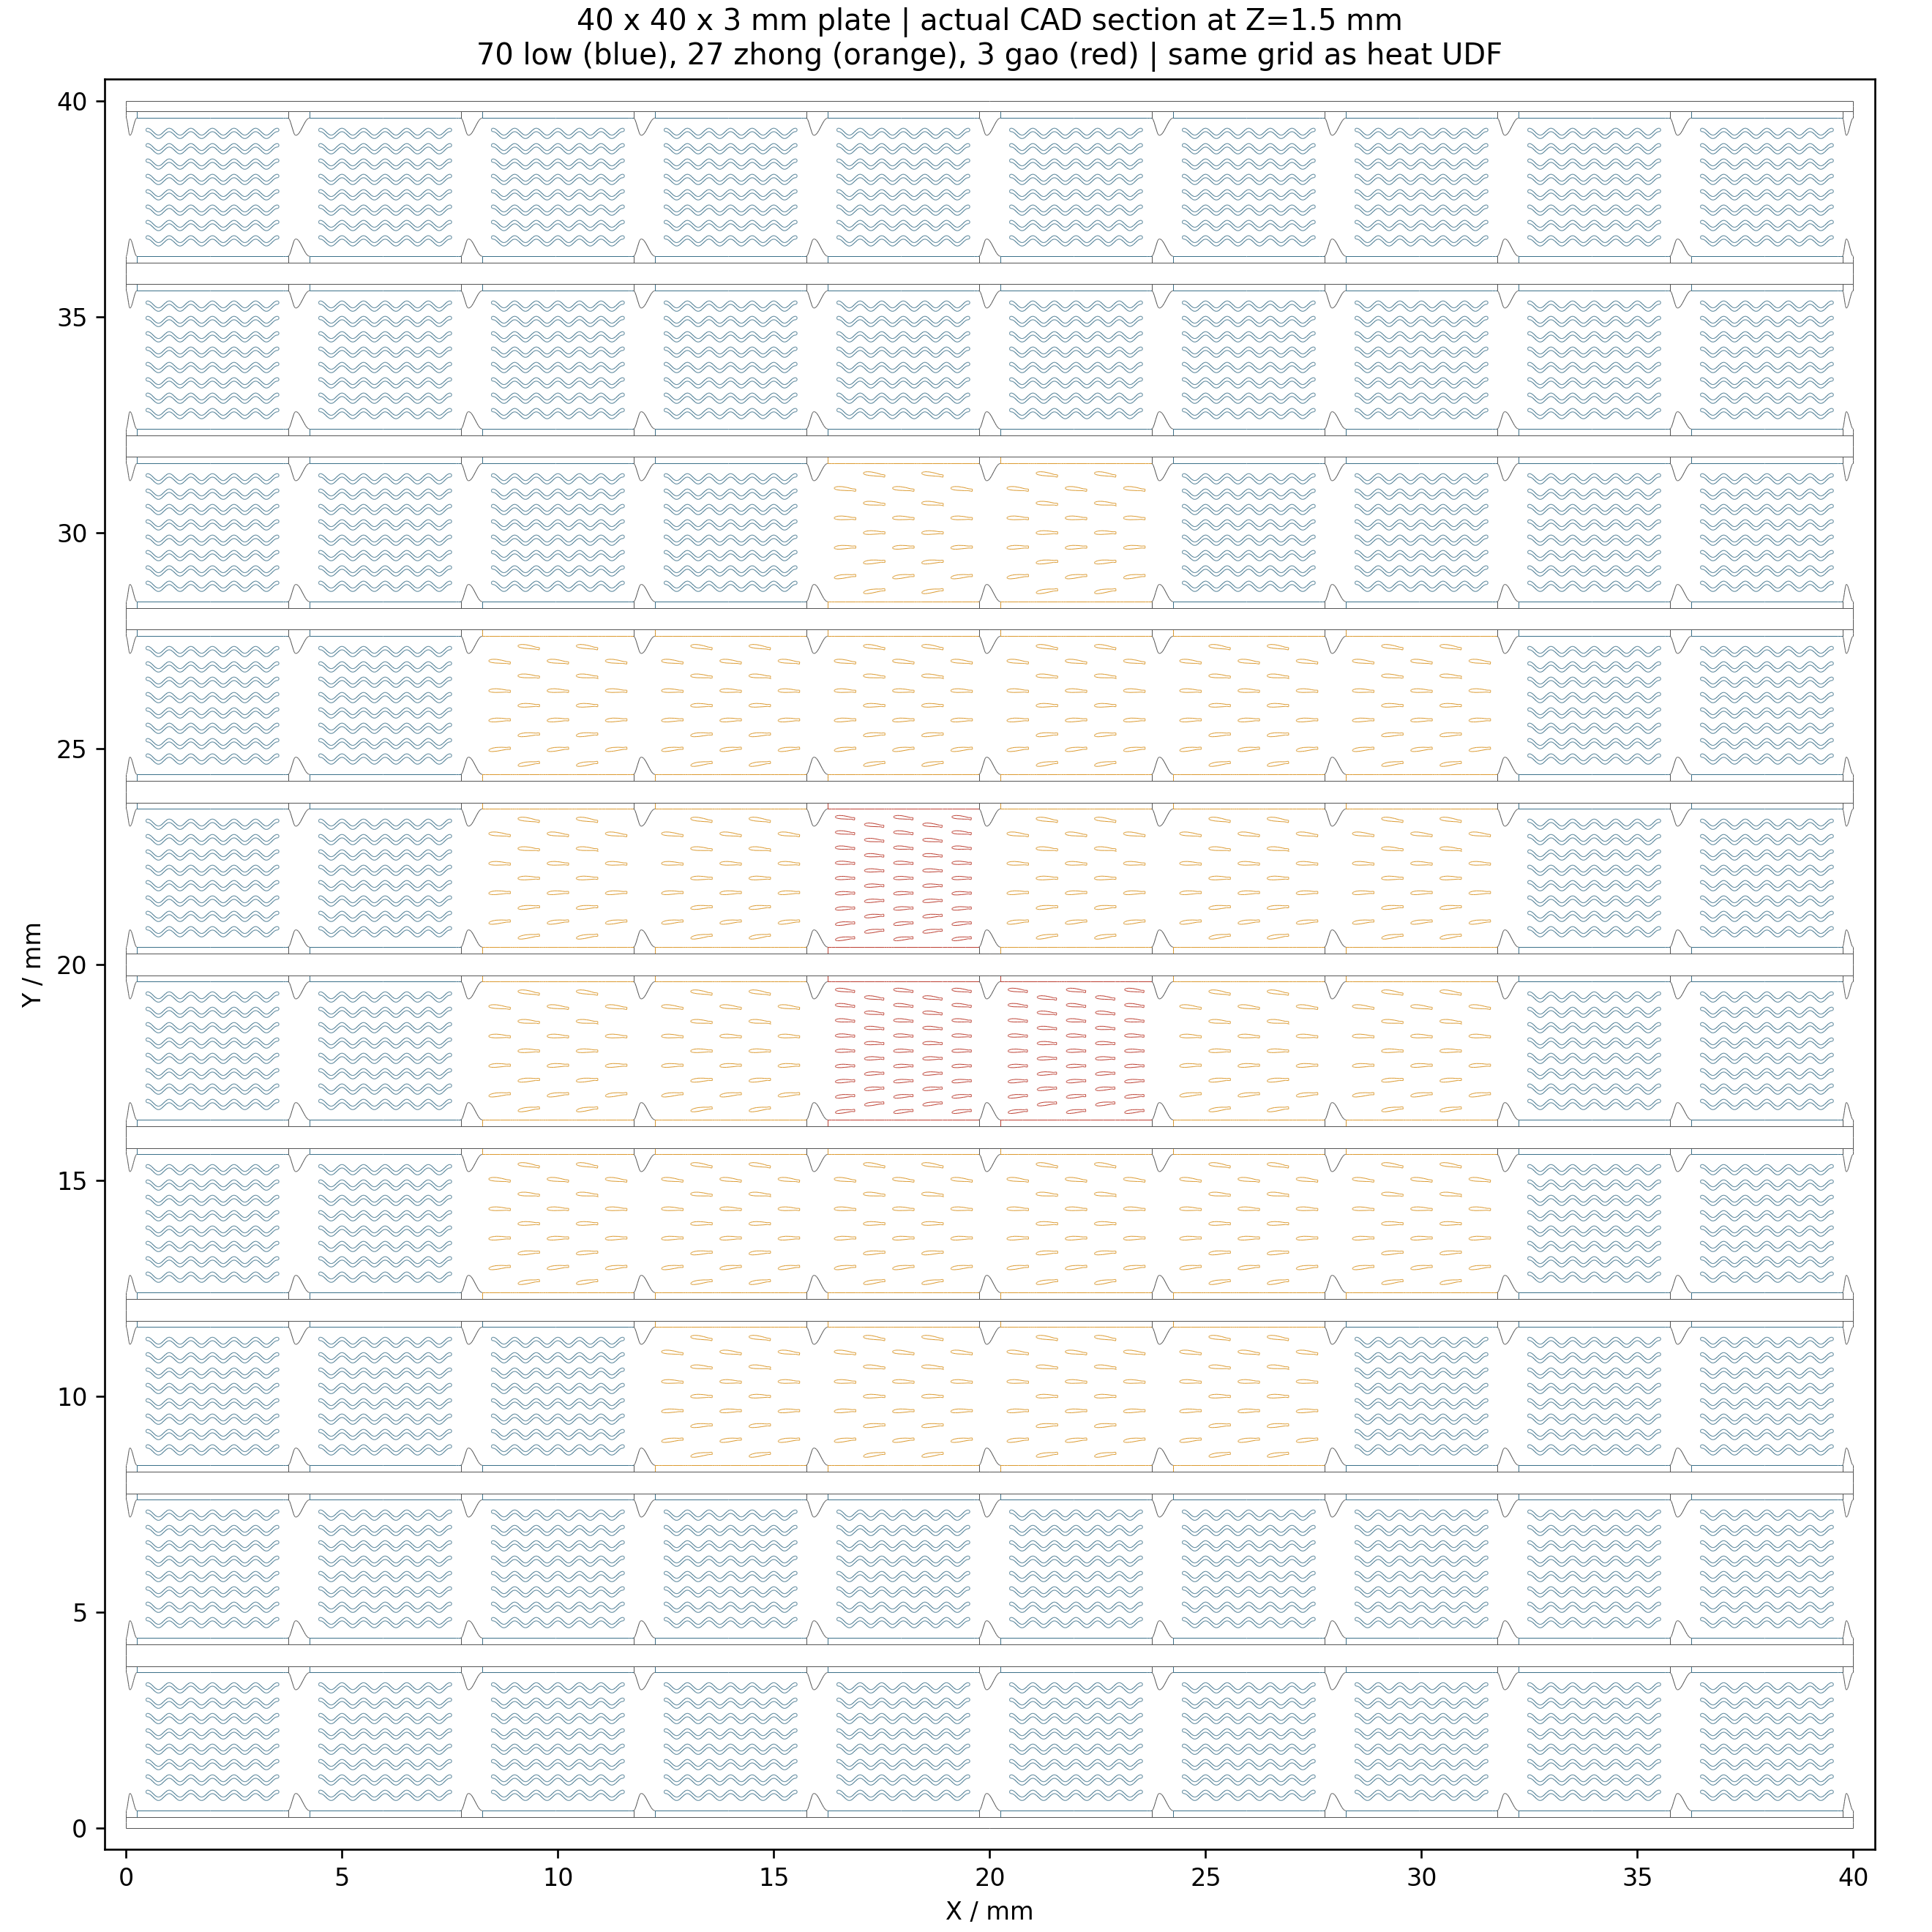
\includegraphics[width=\linewidth,height=88mm,keepaspectratio]{figs/midterm_asset_whole_plate.png}
\caption{当前40 mm整板在 z=1.5 mm 的实际 CAD 截面：70个低负荷、27个中负荷、3个高负荷模块。此图为几何与映射核对，不是整板温度场。}\label{fig:05}
\end{subfigure}\hfill
\begin{subfigure}{0.49\linewidth}\centering
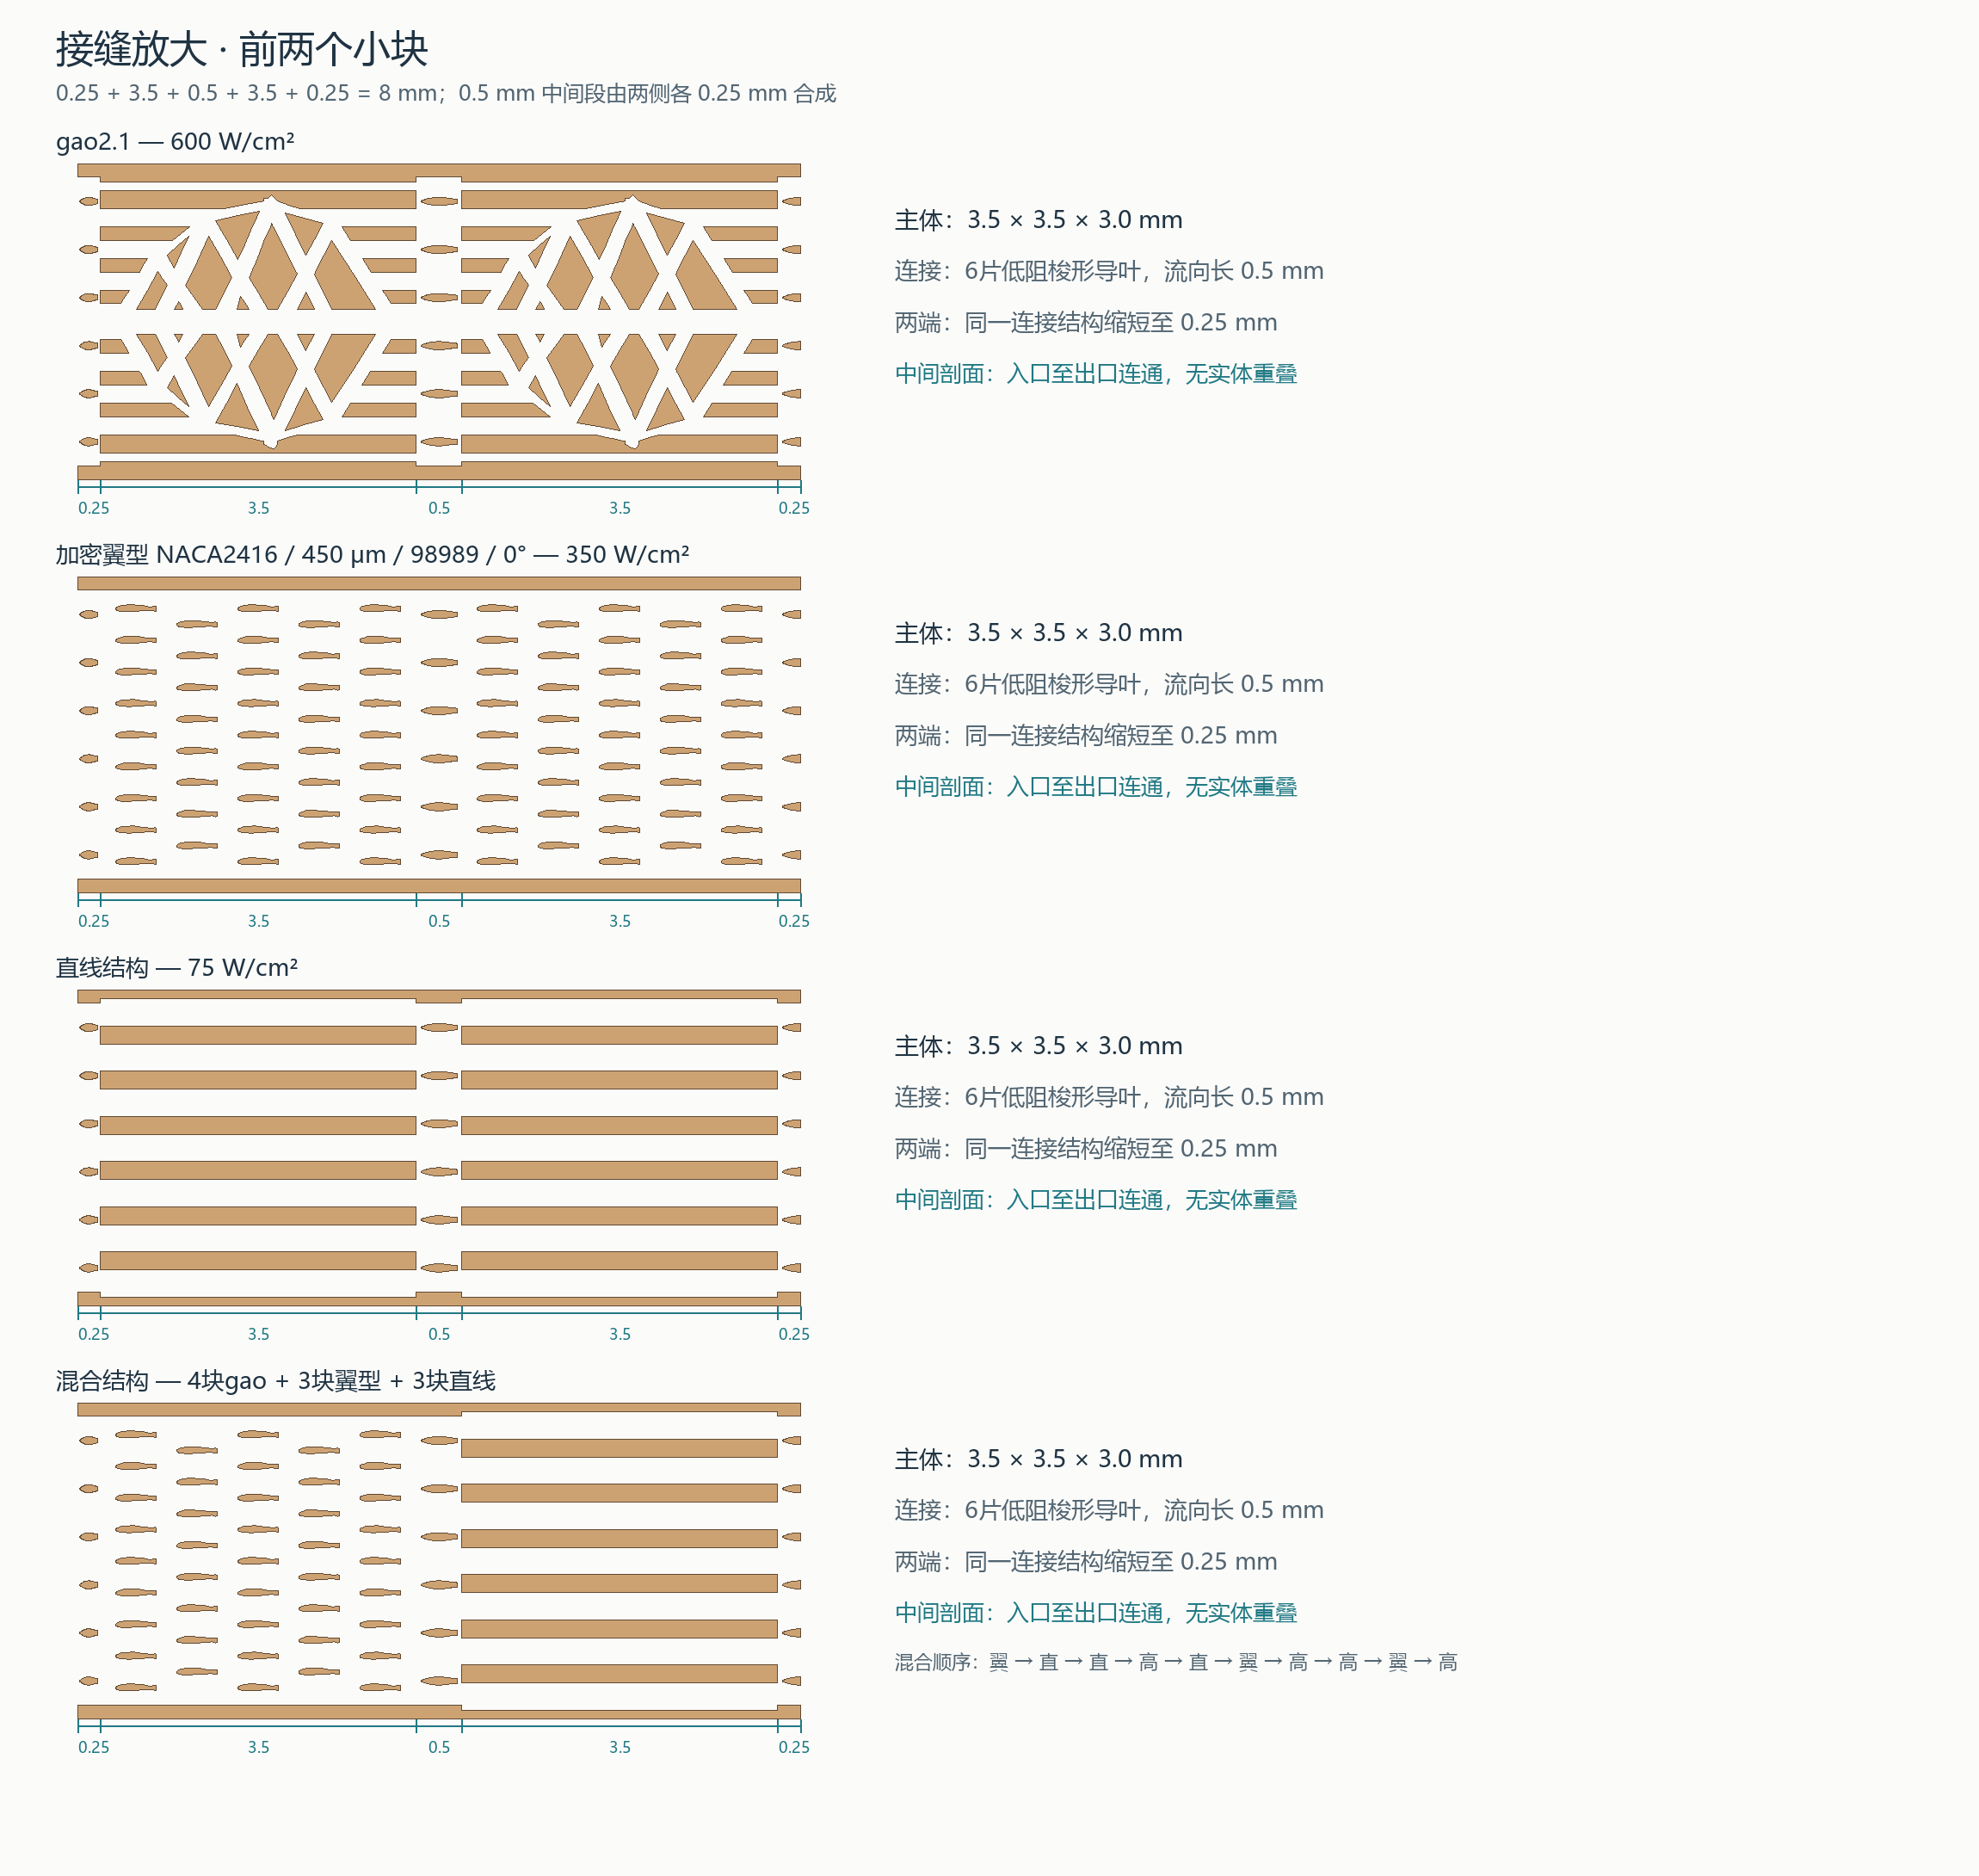
\includegraphics[width=\linewidth,height=88mm,keepaspectratio]{figs/midterm_asset_joint_detail.png}
\caption{40 mm条带装配的接缝放大：主体、六片梭形导叶及内部0.5 mm、端部0.25 mm连接。图注热流为后续主体工况配置，未表示条带已经完成求解。}\label{fig:06}
\end{subfigure}
\caption{整板分区与条带接缝的实际几何}
\label{fig:05-06}
\end{figure}



\subsubsection{三类代表性热负荷工况}
研究按低热负荷、高稳定热负荷和动态波动热负荷组织三类工作模式。低负荷区域重点考察在满足温度要求时控制流动代价；高稳定负荷区域重点考察持续热点和局部传热能力；动态负荷区域重点考察波动下的瞬态温度与后续控制接口。图\ref{fig:12}概括各模式的评价与结构需求，表\ref{tab:07}维护相应边界说明。
\begin{table}[!htbp]
\centering\small
\caption{三类代表性热负荷工作模式}\label{tab:07}
\begin{tabularx}{\linewidth}{CC}
\toprule
\rowcolor{ydzjlight} 工作模式 & 研究侧重点 \\
\midrule
低热负荷 & 满足温度要求并控制流动代价 \\
高稳定负荷 & 持续热点、局部热阻与连接作用 \\
动态波动负荷 & 响应、恢复和泵阀调控接口 \\
\bottomrule
\end{tabularx}
\end{table}

\reportfigure{fig:12}{三类代表性负荷与区域结构配置}{figs/midterm_concept_fig_12.pdf}{\linewidth}
当前整板静态75、350、600 $\mathrm{W/cm^2}$ 三档是空间布局参数，三类工作模式则包含时间性质，二者不是完全相同的分类。尤其350 $\mathrm{W/cm^2}$ 只能代表一个负荷等级，不能证明已经覆盖动态变化。后续对照应注明热源是否恒定、变化幅度、持续时间及总功率，建立可复用工况编号。

\subsubsection{CFD数值模型与基本控制方程}
以下方程是描述单相流动与共轭传热的通用物理基础，用于说明变量和守恒关系；它们不意味着项目已采用全部高阶物理项或所有模型假设均已验证。已读取的代表性物性对照案例采用三维、层流、能量方程及温度相关水物性；整板规划沿用层流和共轭传热思路。不同工况的稳态或瞬态选择、离散格式和求解容差应逐案例确认，表\ref{tab:03}保留具体配置。

对密度可能随温度变化的单相流体，质量守恒写为
\begin{equation}\frac{\partial\rho}{\partial t}+\nabla\cdot(\rho\bm u)=0.\label{eq:mass}\end{equation}
其中 $\rho$ 为密度，$\bm u$ 为速度，$t$ 为时间。只有在恒密度近似下才可简化为 $\nabla\cdot\bm u=0$。温度相关密度启用后，瞬态质量诊断应计入储存项。
\begin{equation}\begin{aligned}
\frac{\partial(\rho\bm u)}{\partial t}+\nabla\cdot(\rho\bm u\otimes\bm u)
&=-\nabla p+\nabla\cdot\bm\tau+\rho\bm g,\\
\bm\tau&=\mu\left[\nabla\bm u+(\nabla\bm u)^{\mathsf T}-\frac23(\nabla\cdot\bm u)\bm I\right].
\end{aligned}\label{eq:momentum}
\end{equation}
$p$ 为压力，$\mu$ 为动力黏度，$\bm g$ 为重力加速度，$\bm I$ 为单位张量。该式适用于牛顿流体、采用 Stokes 假设的黏性应力表述；代表性案例关闭重力。层流模型能否覆盖未来参数范围，应结合雷诺数与流动现象重新判断。

在低马赫数、忽略黏性耗散与压力功、无相变条件下，流体显热方程可表为
\begin{equation}
\frac{\partial(\rho h_f)}{\partial t}+\nabla\cdot(\rho\bm u h_f)
=\nabla\cdot(k_f\nabla T_f)+s_f,
\quad h_f(T)=\int_{T_0}^{T}c_p(\theta)\,\mathrm d\theta.\label{eq:fluidenergy}
\end{equation}
$T_f$ 为流体温度，$k_f$ 为导热系数，$c_p$ 为定压比热，$s_f$ 为体积热源，$T_0$ 为焓参考温度。表面热流边界与体积热源的单位不同，不能混用。温度相关比热时，显热应由积分获得，不宜始终采用常数 $c_p\Delta T$。
\begin{equation}
\rho_s c_s\frac{\partial T_s}{\partial t}=\nabla\cdot(k_s\nabla T_s)+s_s.\label{eq:solidenergy}
\end{equation}
该式描述固体蓄热与导热，$\rho_s,c_s,k_s,T_s,s_s$ 分别为固体密度、比热、导热系数、温度和体积热源。整板当前规划采用铜，具体材料常数或温度函数待团队确认。在无接触热阻界面上，以同一个由固体指向流体的法向 $\bm n$ 表示连续条件：
\begin{equation}
T_s=T_f,\qquad -k_s\nabla T_s\cdot\bm n=-k_f\nabla T_f\cdot\bm n.\label{eq:interface}
\end{equation}
式\eqref{eq:interface}同时约束温度和热流；若后续引入接触热阻，则需改用温度跳跃条件。实际边界配置见表\ref{tab:03}；代表算例与整板规划分别记录，不能仅以控制方程替代实际边界。
\begin{table}[!htbp]
\centering\small
\caption{CFD工况与边界条件维护表}\label{tab:03}
\begin{tabularx}{\linewidth}{lYY}
\toprule
\rowcolor{ydzjlight} 设置 & 已读取案例或当前规划 & 待确认范围 \\
\midrule
模型 & 三维、层流、能量方程 & 代表性物性对照已用；新参数范围需复核适用性。 \\
入口 & $2\,\mathrm{m/s}$，$300\,\mathrm K$ & 当前整板规划沿用历史参数；局部最终对照另核。 \\
出口 & 表压0 Pa，回流$302\,\mathrm K$ & 当前整板规划，不能外推至全部历史案例。 \\
固体 & 铜 & — \\
水物性 & REFPROP拟合，280--360 K & 拟合评估压力101325 Pa；记录启用函数版本。 \\
热边界 & 空间三档映射；动态时序另设 & — \\
求解类型 & 物性对照：瞬态；整板规划：稳态 & — \\
数值格式 & 物性对照：SIMPLE，一阶隐式时间格式 & — \\
残差目标 & 物性对照：连续性/速度$10^{-3}$，能量$10^{-6}$ & 每步最多20次内迭代；生产样本准入须另确认。 \\
重力/操作压力 & 代表性案例关闭重力；101325 Pa & — \\
\bottomrule
\end{tabularx}
\end{table}



\subsubsection{网格划分与检验方法}
团队已开展多轮网格检验，重点关注翼型尾部、狭窄间隙和连接区域，采用局部加密并检查网格质量。尾部剪切与回流区域对压力损失和速度梯度较敏感，单纯增加全域单元数不一定能获得相同的局部解析能力。网格质量通过是计算准备条件，网格无关性则需要比较一致物性、边界、统计时间和收敛条件下的响应量，两者不能互相替代。


具体诊断结果见第三部分。

\subsubsection{温度相关物性 UDF 与热源设置}
水物性实现已进行修正和对照，当前可用拟合 UDF 根据温度返回密度、动力黏度、导热系数和比热，比热积分与显热使用同一多项式。已读取版本声明物性拟合压力为 $101325\,\mathrm{Pa}$、材料温度范围为 $280$--$360\,\mathrm{K}$。该压力是物性评估条件，不表示流动压力场被固定。已排查修正的旧物性问题作为方法改进背景保留，不作为当前主要研究障碍。表\ref{tab:05}记录当前物性与热源配置，空间映射见图\ref{fig:05}；实际区域动态轨迹仍待归档。
\begin{table}[!htbp]
\centering\small
\caption{当前物性模型、热源UDF与实现核对}\label{tab:05}
\begin{tabularx}{\linewidth}{lYY}
\toprule
\rowcolor{ydzjlight} 类别 & 已知配置或核对值 & 适用边界与待补项 \\
\midrule
密度 & $996.556916\,\mathrm{kg/m^3}$（300 K） & water\_rp\_density；仅当前拟合版本。 \\
比热 & $4180.636970\,\mathrm{J/(kg\cdot K)}$（300 K） & water\_rp\_cp；焓由相同比热积分。 \\
动力黏度 & $8.537430\times10^{-4}\,\mathrm{Pa\cdot s}$（300 K） & water\_rp\_viscosity。 \\
导热系数 & $0.609500\,\mathrm{W/(m\cdot K)}$（300 K） & water\_rp\_conductivity。 \\
拟合范围 & 280--360 K，101325 Pa & 物性拟合条件；超范围需扩展或更换模型。 \\
实现对照 & 共同0.137 s：加热面最高温差约$3.197\times10^{-6}$ K & 同初场、步长；不是绝对物理精度验证。 \\
静态空间热源 & 75/350/600 W/cm$^2$；70/27/3格 & 整格加热2640 W；主体面积加热2021.25 W。 \\
动态热源 & 已探索随机波动、趋势与峰值 & — \\
\bottomrule
\end{tabularx}
\end{table}

代表性对照继承同一 $0.1\,\mathrm{s}$ 初场，以 $0.001\,\mathrm{s}$ 步长推进，在共同 $0.137\,\mathrm{s}$ 比较拟合与实时 REFPROP 实现：加热面最高温度差约 $3.197\times10^{-6}\,\mathrm{K}$，面积平均压降差绝对值约 $0.009682\,\mathrm{Pa}$。这些结果支持该案例下两种物性实现的一致性，并不证明所有边界、全部物理模型或实验精度。共同前37步的接口计时比约11.50仅属于物性实现对照，不能写成代理模型加速比。

非均匀热源分为空间映射与时间演化两类。当前整板静态布局为70个低负荷、27个中等负荷和3个高负荷格，对应75、350和600 $\mathrm{W/cm^2}$。按完整 $4\,\mathrm{mm}\times4\,\mathrm{mm}$ 格加热，总输入为2640 W；若只加热 $3.5\,\mathrm{mm}\times3.5\,\mathrm{mm}$ 主体，总输入为2021.25 W。二者是不同覆盖定义，不能把后一面积与前一功率同时使用。映射代码已有中心位置、数量和总热量检查记录，当前整板几何说明进一步核对了模块与热源布局。
\noindent 空间热源对应图~\ref{fig:05}中的实际模块分类；实际区域动态热源序列尚待补入，不能由静态热流等级代替时间变化。


\paragraph{从接口学习到数值自检}
前期学习温度读取与物性接口并完成初步编写；正式的 UDF 修改、编译及代表算例验证属于本阶段工作。以下流程图用于说明实现方法，不代表接口学习阶段已经完成全部校验。
密度、黏度、导热系数采用 \texttt{DEFINE\_PROPERTY} 和 \texttt{C\_T(c,t)}；
比热采用 \texttt{DEFINE\_SPECIFIC\_HEAT}，同时返回 $c_p(T)$ 和其积分显焓，满足
$\mathrm dh/\mathrm dT=c_p$。编译通过只说明接口可用，仍需检查适用温区、数值与变化趋势。
图~\ref{fig:udf-interface}承接这一学习过程。

\begin{figure}[!htbp]\centering
\begin{subfigure}[t]{.49\linewidth}\centering
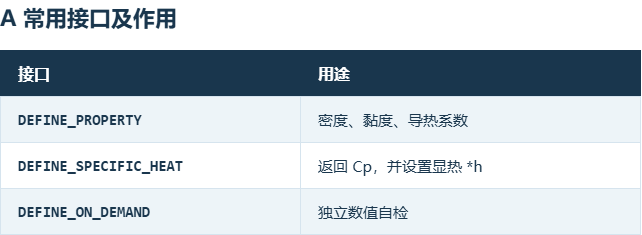
\includegraphics[width=\linewidth]{figs/udf_learning_interfaces_a.png}
\caption{常用接口及作用}
\end{subfigure}\hfill
\begin{subfigure}[t]{.49\linewidth}\centering
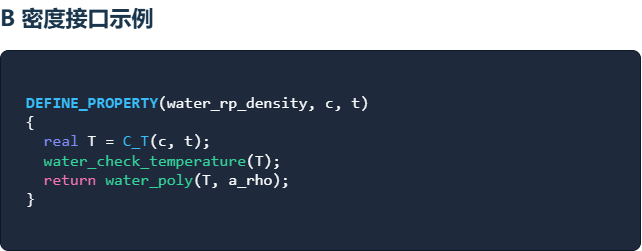
\includegraphics[width=\linewidth]{figs/udf_learning_interfaces_b.png}
\caption{密度接口示例}
\end{subfigure}

\vspace{3mm}
\begin{subfigure}[t]{.49\linewidth}\centering
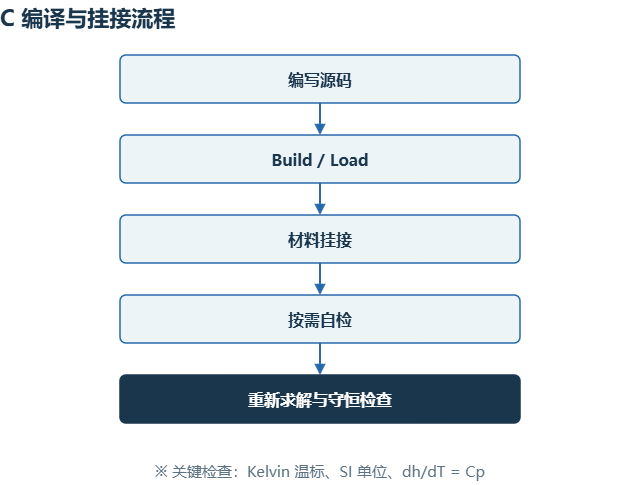
\includegraphics[width=\linewidth]{figs/udf_learning_interfaces_c.png}
\caption{编译与挂接流程}
\end{subfigure}\hfill
\begin{subfigure}[t]{.49\linewidth}\centering
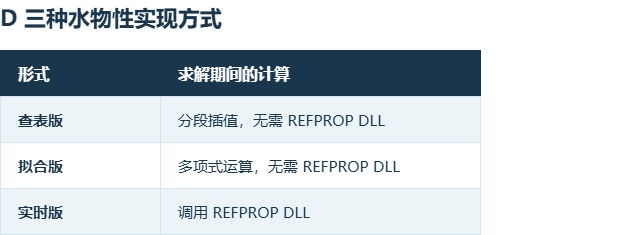
\includegraphics[width=\linewidth]{figs/udf_learning_interfaces_d.png}
\caption{三种水物性实现方式}
\end{subfigure}
\caption{水物性 UDF 的温度输入、函数接口、材料挂接与自检流程；正式修改和核验属于本阶段工作。}\label{fig:udf-interface}
\end{figure}

物性拟合精度与同一时刻的求解对照属于平台校验结果，见第三部分。

\subsubsection{数值仿真自动化流程}
自动化探索覆盖参数配置、几何生成、流体域处理、网格划分、求解配置、监测输出与结果归档。批量计算流程已初步建立，但不同结构的实体有效性、局部网格和求解收敛仍需检查，不能把脚本正常退出等同于样本可靠。每个算例应绑定唯一几何标识、物性版本、边界配置、网格文件及原始监测表，以支持后续复现。

图\ref{fig:11}概括自动化流程与样本准入关口。后续拟在数据集建设中增加样本准入规则：不满足残差、质量守恒、能量平衡或温度范围要求的结果应保留异常标签，重新计算或单独记录，不直接进入训练。已经完成的自动化基础为流程初步贯通，覆盖全部几何和全部工况的稳健批处理仍属于持续完善内容。
\reportfigure{fig:11}{数值仿真自动化与样本质量检查流程}{figs/midterm_concept_fig_11.pdf}{\linewidth}

\subsubsection{流动与传热性能评价指标}
基本流动尺度采用水力直径和雷诺数：
\begin{equation}
D_h=\frac{4A_c}{P_w},\qquad Re=\frac{\rho U_bD_h}{\mu}.\label{eq:re}
\end{equation}
$A_c$ 为选定截面的流通面积，$P_w$ 为湿周，$U_b$ 为体积平均速度。复杂扰流结构的代表截面与物性参考温度必须统一，避免比较对象使用不同定义。平均换热系数和努塞尔数可定义为
\begin{equation}
h_{\mathrm{eff}}=\frac{Q_{sf}}{A_{sf}(\overline T_{sf}-T_{b,\mathrm{ref}})},\qquad Nu=\frac{h_{\mathrm{eff}}D_h}{k_{f,\mathrm{ref}}}.\label{eq:nu}
\end{equation}
$Q_{sf}$ 为固液界面实际传热量，$A_{sf}$ 为对应面积，$\overline T_{sf}$ 为界面面积平均温度，$T_{b,\mathrm{ref}}$ 为声明的流体参考温度。该式为整体等效定义，非均匀或瞬态条件下必须明确平均方式；流体出口温度宜采用质量流量加权，回流时需声明统计规则。
\begin{equation}\begin{aligned}
R_{\theta,\max}&=\frac{T_{w,\max}-T_{\mathrm{in}}}{Q_{\mathrm{in}}},&
\Delta p_s&=\overline p_{\mathrm{in},A}-\overline p_{\mathrm{out},A},\\
P_h&=\Delta p\,\dot V,& P_e&=\frac{P_h}{\eta}.
\end{aligned}\label{eq:resistance}
\end{equation}
$T_{w,\max}$ 为指定受热壁面最高温度，$Q_{\mathrm{in}}$ 为输入热功率，$\dot V$ 为体积流量，$\eta$ 为泵与驱动的综合效率。稳态 $R_{\theta,\max}$ 可用于温升比较；瞬态同一比值含有历史和蓄热影响，不能直接解释为静态热阻。面积平均静压差用于流阻对照，但存在截面速度差异或回流时，泵送评价应补充总压或机械能通量，并计入系统管路与阀门损失。
\begin{equation}
\Delta T_A=T_{w,\max}-T_{w,\min},\qquad
\sigma_{T,A}=\left[\frac{1}{A}\int_A(T_w-\overline T_{w,A})^2\,\mathrm dA\right]^{1/2}.\label{eq:uniformity}
\end{equation}
$A$ 为统一的受热面评价区域，二者分别反映极差和整体温度分散程度。表\ref{tab:06}给出指标维护模板。项目后续将优先保证指标含义与统计位置一致，再开展性能排序。
\begin{table}[!htbp]
\centering\small
\caption{热工与流动性能指标定义及维护模板}\label{tab:06}
\begin{tabularx}{\linewidth}{CC}
\toprule
\rowcolor{ydzjlight} 指标 & 统计定义 \\
\midrule
$T_{w,\max}$ & 指定受热面最高温度/K \\
$\overline T_{w,A}$ & 受热面面积平均/K \\
$\Delta T_A,\sigma_{T,A}$ & 温度极差与面积标准差/K \\
$R_{\theta,\max}$ & 最高温升/输入功率，K/W \\
$h_{\mathrm{eff}},Nu$ & 界面传热与声明流体参考温度 \\
$\Delta p_s$ & 进出口面积平均静压差/Pa \\
$P_h,P_e$ & 水力功与泵电功率/W \\
守恒误差 & 质量与能量平衡；瞬态含储存项 \\
\bottomrule
\end{tabularx}
\end{table}

\FloatBarrier
\subsection{方向一：连接结构的设计与验证方法}
\label{ch:connection}
\subsubsection{区域化冷板设计思路}
方向一针对不同热负荷区域散热需求不同、模块连接可能引入额外流动损失的问题，将整体冷板拆分为可配置的基本单元，并研究连接段如何组织上游流动进入下游结构。针对多热源模块的液冷研究也表明，按热源位置布置强化结构比全域均匀强化更有效\cite{ref2}。区域化设计并不意味着单元间热量和流量完全独立：固体横向导热、上游流体温升和行级压力耦合仍会影响局部工作点。因此，局部结构适配和连接整流应作为一个组合问题评价。

项目已有整体分区与单元设计思路、代表性小模型计算和连接方案库。既有记录表明连接方向及评价方法已明确，但尚无连接段成对仿真结果；几何装配资料进一步说明可采用六片梭形导叶连接，未提供相同主体、相同工况下的连接收益。本节先说明设计思路与对照组织，再说明连接验证的输入与缺口；已有单元结果见第三部分。

\subsubsection{局部结构对照的设计}
前期探索了常规、仿生及翼型小块，随后集中整理了翼型专题与参数分组方案。完整分组数据尚未提供，历史分支只按实际保存条件使用，结果按共同热流工况、六翼型基准和已保存代表分支分别列出，并注明平均温度定义、时间、流量与物性条件\cite{stagereports}。

各分支的保存条件与实测指标见第三部分，本节只说明对照是如何组织的。

\subsubsection{基本单元与连接结构}
基本单元按4 mm节距组织，当前整板版本将3.5 mm主体布置在格中心，行内连接长0.5 mm，两端各保留0.25 mm；条间填充与边缘处理用于满足整体外形尺寸。连接段的功能不仅是几何拼接，还包括将不同主体的出口速度分布调整为可接受的下游入口条件，降低突变接口造成的流动偏置。图\ref{fig:13}给出四条条带装配的实际内部截面。

已有连接方案库包含梭形导叶、蜂窝整流格、双排导叶及螺旋槽等版本，方案存在本身不代表均已完成性能计算。当前四条40 mm验证装配记录明确采用低阻梭形直导叶、保留六片导叶和横向轮廓，并对流向长度进行缩短。表\ref{tab:08}仅记录这一可追溯的装配版本；团队已验证连接方案与此版本的对应关系、最终成果版本号仍需确认，不能因多个目录出现“最终版”便推定为同一性能对照对象。
\begin{table}[!htbp]
\centering\small
\caption{可追溯连接装配版本及最终对照参数模板}\label{tab:08}
\begin{tabularx}{\linewidth}{CC}
\toprule
\rowcolor{ydzjlight} 参数 & 当前40 mm条带记录 \\
\midrule
连接型式 & 低阻梭形直导叶 \\
导叶数量 & 6片 \\
内部/端部长 & 0.5/0.25 mm \\
外壳宽/高 & 3.5/3.0 mm \\
通腔宽/高 & 3.2/2.5 mm \\
侧壁/上下壁 & 0.15/0.25 mm \\
基准连接 & — \\
\bottomrule
\end{tabularx}
\end{table}


\begin{figure}[!htbp]\centering
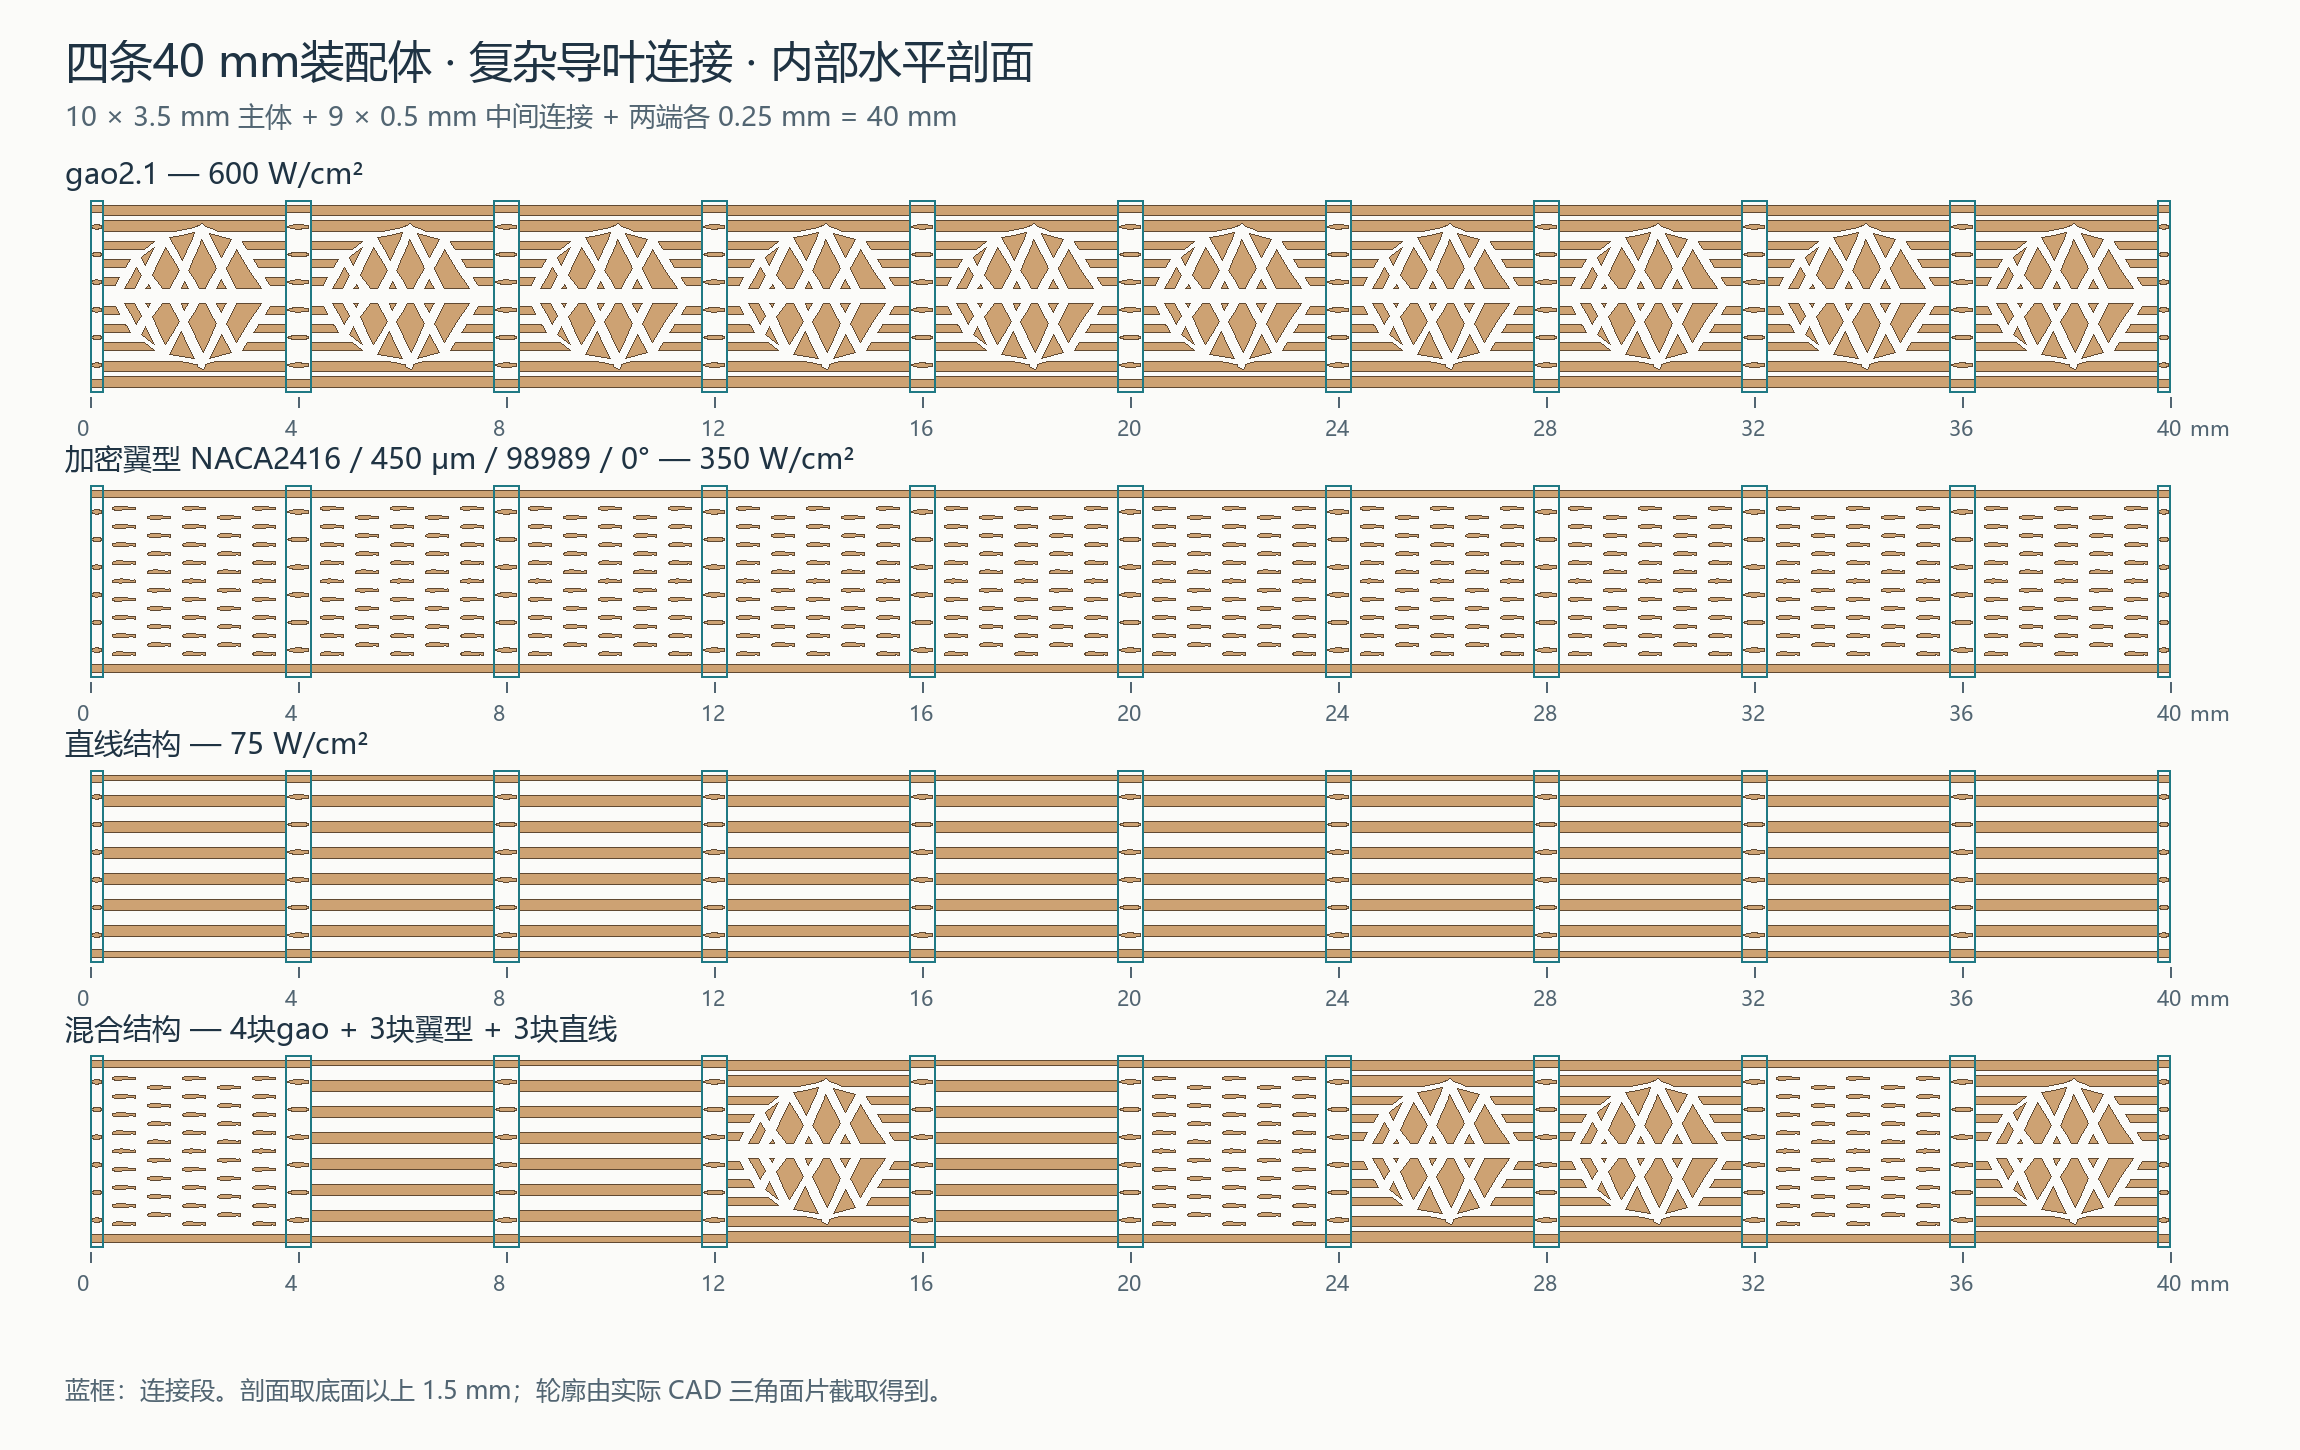
\includegraphics[width=\linewidth,height=125mm,keepaspectratio]{figs/midterm_asset_strip_overview.png}
\caption{四条40 mm装配的实际内部截面，包含gao2.1、翼型、直线及混合排列；用于几何准备和接口检查。}\label{fig:13}
\end{figure}


\subsubsection{连接结构的验证方案}

目前尚未形成连接段仿真结果，当前可核对的是设计目标、候选方案与装配几何。
局部小模型温度和水力性能不能代替连接段“有／无整流”的成对验证。
下一步需在相同主体、相同热负荷和相同入口约束下，比较连接前后截面的流量、速度均匀性与压降，
并输出下游受热面温度。若采用固定泵功，应由各自水力特性确定运行点，不能只固定入口流量后宣称等泵功改善。
现有条带几何可作为计算输入，但仍需流体域、共享拓扑、网格和守恒检查\cite{stagereports}。


表\ref{tab:09}建立基准与确定方案的最终对照模板。当前可以确认的是已有连接候选和可追溯装配；尚不能确认连接本身能否改善指定指标、其幅度及适用负荷范围。填写表格时，应同时列出受热面最高温度、面积平均温度或均匀性、压降及泵送代价，对不利变化也应如实记录。
\begin{table}[!htbp]
\centering\small
\caption{连接结构与基准结构的成对性能比较模板}\label{tab:09}
\begin{tabularx}{\linewidth}{CC}
\toprule
\rowcolor{ydzjlight} 指标 & 比较条件 \\
\midrule
$T_{w,\max}$/K & 同热源、同流量或同泵功。 \\
$\overline T_{w,A}$/K & 相同受热面及统计时刻。 \\
$\sigma_{T,A}$/K & 相同区域及面积加权。 \\
$\Delta p$/Pa & 声明静压、总压或能量口径。 \\
$R_\theta$/(K/W) & 声明稳态与总热功率。 \\
$P_h$/W & 流量与系统压力范围一致。 \\
优势与代价 & 仅根据归档数据填入，不编造百分比。 \\
\bottomrule
\end{tabularx}
\par\smallskip\begin{minipage}{\linewidth}\footnotesize 局部单元性能已在前文给出；本表专用于连接段成对验证，不能用不同主体或不同工况的小模型数据代填。\end{minipage}
\end{table}



表\ref{tab:09}同时保留压力代价与热响应两个维度。优势分析应回答：改善是否出现在局部连接附近，是否延续到下游单元，是否随入口流量变化，以及是否以额外阻力为代价。如果不同指标呈现权衡，可以表述为特定工况下的综合适用性，而不能用一个未经声明权重的综合分数掩盖取舍。
\pending{需补入确定方案的成对原始结果、工况编号、温度与压力监测位置、比较约束及误差；不得填写未经提供的提升百分比。}

\subsubsection{流动传热机理讨论}
连接段可能通过改变截面收缩与扩张过程、引导横向速度分量和调整下游入口分布影响传热。若导叶使入口偏流减弱，下游部分通道可能获得更均衡供液；若强化局部混合，则可能改变温度梯度和边界层发展。这些是需要由速度、流量分配与温度证据验证的机理假设，不能因为设置了导叶便认定所有机制已经成立。

建议沿连接前、连接中和连接后三个位置提取截面速度分布与局部压力，比较不同支路流量及下游受热面温度。若观察到回流减弱，需要同时确认涡区大小、持续位置与流量通行情况，而不只展示某一条流线。若温度改善发生于下游较远处，应讨论流体温升、固体导热和入口重新发展共同作用，避免将全部变化归因于单一局部现象。

由于泵送功率取决于流量和系统阻力，局部压降降低不必然等于系统电能降低；不同进出口速度分布还可能改变静压与总压差的对应关系。后续机理解释将结合已建立的多口径压力核验方法，选择与研究问题匹配的压力评价。几何、流动、热响应与能耗之间的关联需由成对结果支持，当前不以示意箭头替代连接机理证据。

\subsection{方向二：动态调控的方法与模型}
\subsubsection{动态热负荷问题定义}
方向二关注热负荷在空间和时间上变化时，如何通过有限数量的泵阀执行器调节冷却供给，使热点温度受到约束，同时改善温度分布并控制泵送代价。与稳态结构比较不同，动态控制的评价对象是一段完整响应过程，包括扰动开始、控制动作、温度过渡及恢复，而不是单一时刻的最低温度。

可将受热面划分为区域 $A_i$，用 $q_i''(t)$ 描述第 $i$ 区热流密度。项目采用十行单向流路的初步规划，行级控制对应的是一组区域的集体供液，不能独立指定100个单元的流量。沿流向的流体升温、横向固体导热以及共用供回水压力使控制对象具有耦合性。相邻区域的温度响应可能受到同一控制动作影响，这正是协同控制需要处理的问题。

当前已有基本架构和简化对象上的 PID 闭环时序，尚未形成实物泵阀或多行耦合系统的完整性能数据。后续研究需首先界定允许最高温度、反馈区域、采样周期和泵阀限制，再比较控制算法。未知温度约束和实际硬件特性均保留待确认，不预设能够满足的性能指标。


基于热容惯性、输运滞后及执行器限幅，控制方向提出分层递阶与独立约束的控制框架，
见图~\ref{fig:control-month1}。感知、预测、决策和执行是功能划分，
其中预测和增益调度仍属方案；当前量化证据来自后文简化 PID，而非全部层级已经实现。
流量相关换热与泵送成本需由实际通道和设备特性辨识，不能把幂律指数或泵功立方关系视为所有流况的既定结论。

\begin{figure}[!htbp]\centering
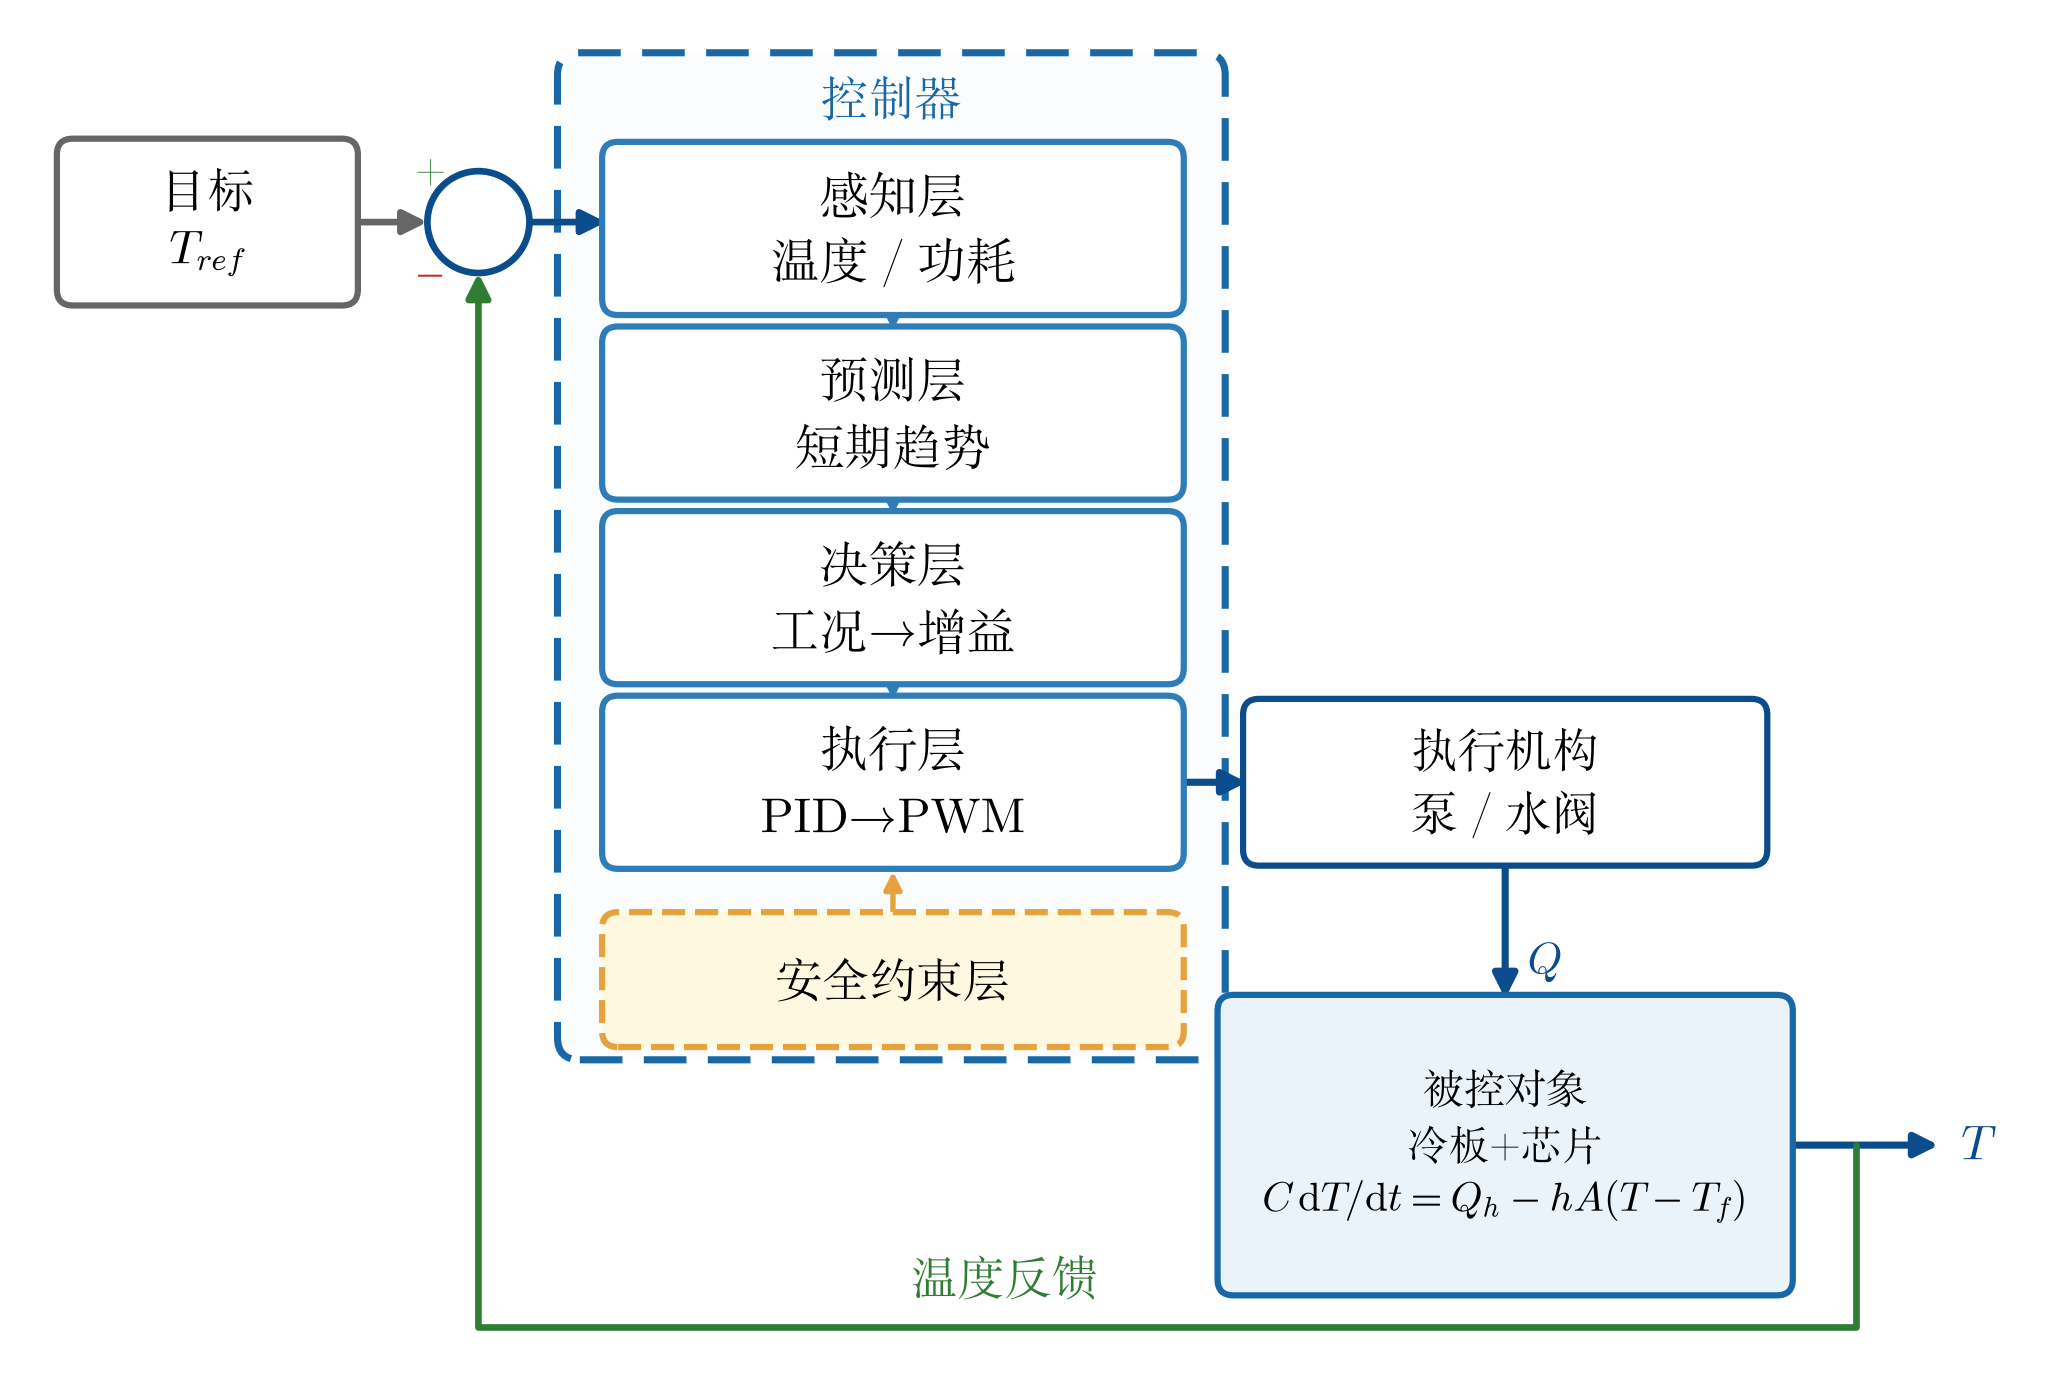
\includegraphics[width=\linewidth]{figs/midterm_monthly1_13_控制框架框图.png}
\caption{感知、预测、决策、执行与独立安全约束框架，作为后续系统架构方案。}\label{fig:control-month1}
\end{figure}
\subsubsection{双泵与行级阀门控制架构}
系统基本方案为双泵与行级出口阀门协同调控，利用区域温度反馈决定泵工作状态和各行阀门开度。泵主要影响供液压力或总流量，阀门主要改变各行水力阻力；两者通过公共管路作用于全部行，不能简单解释为泵负责温度、阀门负责均匀性而完全独立。图\ref{fig:18}示意系统架构与温度反馈链，表\ref{tab:10}给出输入、状态与输出维护模板。
\reportfigure{fig:18}{双泵与行级出口阀门协同控制架构}{figs/midterm_concept_fig_18.pdf}{\linewidth}
\begin{table}[!htbp]
\centering\small
\caption{动态系统的输入、状态、测量及控制输出}\label{tab:10}
\begin{tabularx}{\linewidth}{CC}
\toprule
\rowcolor{ydzjlight} 类别 & 候选量与物理意义 \\
\midrule
扰动输入 & $q_i''(t)$、入口温度 \\
热状态 & $T_i,T_{f,i}$，区域与流体温度 \\
水力状态 & $\dot V_i,\Delta p$，行流量与供液压力 \\
测量输出 & 区域最高温、代表点或平均温度 \\
控制输出 & 两泵转速/流量指令、行级出口阀开度 \\
约束 & 温度上限、最小流量、动作速率 \\
\bottomrule
\end{tabularx}
\end{table}

当前明确的是双泵和行级阀门的基本框架，两台泵的串并联关系、实际回路分组、阀门数量与可调范围、温度测量方式仍需结合系统方案确认。十行规划通常需要逐行控制接口，但未提供执行器采购或标定记录，因此报告不将“十个实物阀门已安装”作为成果。反馈温度可取区域最高值或代表点，但选择不同统计方式会改变控制动作，需统一记录。

建议后续采用分层协调思路：上层根据最热区域及总需求调节泵供给，下层依据行间需求差异分配阻力，同时施加流量下限和动作速率约束。这是可研究的实现方式，尚不作为已完成算法。需要特别防止阀门同时节流导致泵供给与行流量目标冲突，或某行开启使其他行流量下降。

\subsubsection{动态非均匀热源建模}
一般区域热源可表示为
\begin{equation}
q''(\bm r,t)=\sum_{i=1}^{100}\chi_i(\bm r)\left[q_{i,0}''+a_i s_i(t)\right],\qquad
Q_{\mathrm{in}}(t)=\sum_i A_i q_i''(t).\label{eq:heatmap}
\end{equation}
$\bm r$ 为受热面坐标，$\chi_i$ 为区域指示函数，$q_{i,0}''$ 为基值，$a_i$ 为变化幅度，$s_i(t)$ 为无量纲时间信号。各信号需满足热流非负与目标范围要求。阶跃、脉冲、周期波动和随机轨迹用于分别观察响应速度、恢复能力、周期跟踪与扰动适应性；式\eqref{eq:heatmap}是后续统一建模表达，不代表100区随机独立热源已全部实现。

现有热源 UDF 已探索升温趋势、随机波动与短时峰值。其中读取到的一个历史文件在同一次调用中向同一壁面所有网格面赋相同热流值，因而主要描述时间变化，不能仅凭该文件认定已经实现空间独立波动。团队提供的动态非均匀研究进展作为阶段状态记录，最终需补入实际使用的区域热源文件、版本与输出轨迹，以证明空间差异和时间变化同时存在。

随机热源用于算法比较时，还需要可复现性。同一随机种子本身不足以保证跨计算模式完全一致，因为 UDF 调用次数和并行执行可能不同。后续宜采用预生成热源时间表或按物理时刻索引的确定性映射，将扰动更新绑定到时间步而非不受控的函数调用。控制算法之间应复用同一轨迹和初态，避免以不同扰动比较优劣。这属于热源模型深化任务，并非否定已完成的可行性探索。后续应以同一时间轴保存真实区域负荷与温度；已有简化 PID 的温度信号不等同于区域热流时序。


\subsubsection{最小闭环对象与 PID 控制}

闭环算例采用一阶集总温控对象与增量式 PID（其形式与限幅处理参照经典自动控制与 PID 整定教材\cite{hushousong,astrom,ogata}），共保存1800个采样点，采样周期0.05 s，时间坐标0--89.95 s。
热源输入是 $82\pm12$ $^\circ$C、周期15 s的\textbf{温度信号}，不是 W/cm$^2$ 表示的区域热流；
程序以经验加热系数0.45和随执行量变化的冷却系数0.03--0.20推进温度。
因此，该算例验证抽象冷却动作下的闭环逻辑，不是耦合 Fluent、实物双泵或十行阀门的系统验证。
基础 PID 可写为
\begin{equation}\begin{aligned}
u_i(t)&=\operatorname{sat}\left[u_{i,0}+K_{p,i}e_i(t)+K_{i,i}\int_0^t e_i(\tau)\,\mathrm d\tau+K_{d,i}\frac{\mathrm de_i}{\mathrm dt}\right],\\
e_i&=T_i-T_{i,\mathrm{set}}.
\end{aligned}\label{eq:pid}
\end{equation}
$u_i$ 为冷却动作的抽象量，$u_{i,0}$ 为基准指令，$T_i$ 与 $T_{i,\mathrm{set}}$ 为反馈与设定温度，三个增益分别对应比例、积分和微分作用，$\operatorname{sat}$ 为执行器限幅。若增大 $u_i$ 表示增强冷却，上述误差符号与正比例增益相匹配；阀开度与流量关系仍需标定。该式用于说明连续形式；已有程序采用增量更新，累计误差限幅没有实际进入控制更新，需先修正并复核后再评价抗饱和效果。

\subsubsection{向物理机理融合模型的发展}
后续研究将由简化数学模型逐步过渡至能反映蓄热、流量和压力耦合的物理灰箱模型；这类「物理约束 + 数据驱动」的建模思路在系统辨识与数字孪生方向已有系统讨论\cite{brunton,tao}。对于区域集总温度，在内部温差相对可控、参数经过辨识的条件下，可建立
\begin{equation}
C_i\frac{\mathrm dT_i}{\mathrm dt}=Q_i(t)-G_i(\dot m_i)(T_i-T_{f,i})
-\sum_{j\in\mathcal N_i}G_{ij}(T_i-T_j).\label{eq:rc}
\end{equation}
$C_i$ 为区域等效热容，$G_i=1/R_i$ 为流量相关等效换热热导，$T_{f,i}$ 为流体参考温度，$G_{ij}$ 表示相邻区域导热。式\eqref{eq:rc}描述蓄热、散热和横向耦合，参数不能仅以材料常数直接替代，需要通过 CFD 或响应数据辨识。流体沿程温升明显时，应增加流体状态或分段输运描述，而不能始终使用相同入口温度。

流量分配应满足节点守恒与支路压降一致性。以共用供回液压力的并联行为例，可写
\begin{equation}\begin{aligned}
\sum_i\dot V_i&=\dot V_{\mathrm{tot}},\\
\Delta p_{\mathrm{man}}&=\Delta p_{\mathrm{ch},i}(\dot V_i,T_i)
+\Delta p_{\mathrm{v},i}(\dot V_i,\alpha_i).
\end{aligned}\label{eq:hydraulic}
\end{equation}
$\alpha_i$ 为第 $i$ 行阀门开度，$\Delta p_{\mathrm{man}}$ 为供回液压差；通道和阀门关系由结构、温度及特性曲线决定。泵特性需写为 $\Delta p_{\mathrm p}=F_{\mathrm p}(n,\dot V)$，其中 $n$ 为泵速。式\eqref{eq:hydraulic}适用于所声明的并联拓扑；两泵回路尚未确认，实际网络若不同应重新列式，不先写定串并联结构。

将区域温度、必要流体状态与压力变量组合后，可以形成非线性状态模型，并在特定工作点线性化：
\begin{equation}\begin{aligned}
\dot{\bm x}&=\bm f(\bm x,\bm u,\bm d;\bm\theta),\quad\bm y=\bm g(\bm x,\bm u),\\
\delta\dot{\bm x}&=\bm A\delta\bm x+\bm B\delta\bm u+\bm E\delta\bm d.
\end{aligned}\label{eq:state}
\end{equation}
$\bm x,\bm u,\bm d,\bm y,\bm\theta$ 分别为状态、控制、热负荷扰动、测量输出和待辨识参数；$\bm A,\bm B,\bm E$ 为工作点附近的线性矩阵。该形式是模型发展路线，当前尚未提供经辨识验证的参数矩阵。图\ref{fig:21}用于区分简化反馈、灰箱模型和后续控制比较的关系。
\reportfigure{fig:21}{由简化数学模型向物理机理融合动态模型的演进}{figs/midterm_concept_fig_21.pdf}{\linewidth}

\subsection{方向三：代理模型的构建与评价方法}
\subsubsection{代理模型研究需求的提出}
方向三源于结构与工况研究扩大后的计算需求。高保真 CFD 提供流场、温度场和边界响应，但多参数、多负荷和多次验证需要反复求解，成本包含建模、网格、求解、数据提取以及质量检查。代理模型拟在已声明的参数范围内，以少量计算替代部分重复性能预测，从而支持更密集的分析和控制模型构建。

该方向的核心问题是预测方法是否准确、数据是否足够、物理信息是否带来可验证收益，以及建库和训练成本能否在后续调用中回收。几何参数化用于形成可控样本变化和独立泛化测试，并非把寻找最优几何作为主要目标。当前已确定技术路线并建立部分 CFD 与自动化基础，尚未提供训练完成后的性能结果。

\subsubsection{代表性翼型结构与几何参数化}
已开展的代表性对象包括 NACA2416 等翼型扰流结构。当前40 mm条带装配采用的局部翼型为 NACA2416\_L450um\_98989\_A00deg，记录给出0.45 mm翼型尺度、9/8/9/8/9错列排列、每块43个扰流柱和0度迎角。该配置用于代表性建模与结构审阅，不构成性能最优证明，也不能自动作为全部样本的基准。

后续可将弦长、迎角、排布间距、柱高和翼型类别等作为候选几何变量，同时考虑入口速度或雷诺数、入口温度及热边界。候选变量并不意味着全部都必须进入模型，应通过机理分析和样本可实现性筛选，防止输入维度过高而稀释样本覆盖。参数上下界、单位及生成约束需由团队确认，不能从目录名称推定连续可行域。


代表翼型排布见图\ref{m2:fig:naca-small}，NACA2416统一平面的实际网格见图\ref{fig:08}；这些图没有提供全部弦长、柱高和边界层参数，后续仍需对应几何文件核对。参数改变可能导致最小间隙改变、局部接触或流体域连通性变化，因此几何生成流程需先做可行性检查，再进入批量计算。其方法价值在于建立可复现的参数—几何—网格映射，而非仅生成数量较多的模型文件。

\subsubsection{CFD数据集构建方法}
数据集以算例为基本单位，每条样本应包含输入参数、物性版本、几何版本、网格统计、边界配置、输出指标、质量标签和计算成本。历史算例可用于流程验证和探索，但不同物性、不同时间点或不同压降口径的结果不能未经统一便合并为训练标签。方向三正在构建高保真样本集，尚未确认最终有效样本数。表\ref{tab:12}为候选输入和输出建立统一字典。
\begin{table}[!htbp]
\centering\small
\caption{代理模型候选输入、输出与数据标识}\label{tab:12}
\begin{tabularx}{\linewidth}{CC}
\toprule
\rowcolor{ydzjlight} 类别 & 候选内容 \\
\midrule
几何输入 & 翼型、弦长、迎角、间距、柱高 \\
流动输入 & 入口速度或Re、入口温度 \\
热边界输入 & 热流等级、空间类别、必要时间参数 \\
物理特征 & Re、Pr、Pe、几何比值、简化基线 \\
温度输出 & 受热面最高温、出口混合温度 \\
性能输出 & 压降、热阻或Nu \\
元数据 & 几何ID、网格、物性、守恒、计时 \\
\bottomrule
\end{tabularx}
\end{table}

\reportfigure{fig:24}{高保真CFD样本生成与数据集划分流程}{figs/midterm_concept_fig_24.pdf}{\linewidth}
图\ref{fig:24}概括样本生成、准入和独立测试全过程。建议先建立覆盖主要参数范围的基础样本，再根据误差或信息不足区域补点。训练、验证与测试应按几何或工况组合分组，防止同一几何的近邻样本分散到不同集合导致结果偏乐观；标准化和特征选择仅在训练数据上拟合，超参数选择仅使用验证或分组交叉验证数据。

标签的物理含义需要统一。受热面最高温度、出口混合温度、静压损失、总压损失和热阻描述不同任务，不宜混为一个未定义的“综合性能”。瞬态指标必须注明时刻或统计窗口；稳态样本需记录收敛与热平衡条件。不能将网格敏感性检验中不同单元数产生的差异当作几何差异的学习目标。

\subsubsection{物理机理分析与理论推导路线}
该方向将并行推进物理理论与物理机器学习，两条路径互相支撑而不互相替代。理论路径首先明确流动与换热的控制尺度，讨论几何长度、黏性效应、热扩散和流体输运如何影响性能；数据路径检验这些解释能否在有限样本中提高预测与泛化。相关推导正在推进，不在报告中声称已获得适用于全部结构的闭式关联式。

除 $Re$ 外，可考虑普朗特数和佩克莱数：
\begin{equation}
Pr=\frac{\mu c_p}{k_f},\qquad Pe=Re\,Pr,\qquad
t_{\mathrm{adv}}=\frac{L}{U_b},\quad t_{\mathrm{diff}}=\frac{L^2}{a},\quad a=\frac{k}{\rho c}.\label{eq:scales}
\end{equation}
$Pr$ 表示动量与热扩散的相对尺度，$Pe$ 表示对流与热扩散的相对作用；$L$ 为声明的特征长度，$a$ 为对应介质热扩散率。固体与流体应分别选取物性和长度，不能用同一 $a$ 代表整个共轭域。这些量可用于解释不同负荷与流量下的响应，但能否作为有效特征需经独立模型比较。

在稳态、无其他热损失且固液能量闭合时，冷却液输运热量满足
\begin{equation}
Q_{\mathrm{in}}=\dot m\left[h_f(T_{\mathrm{out},b})-h_f(T_{\mathrm{in}})\right].\label{eq:bulkenergy}
\end{equation}
$\dot m$ 为质量流量，$T_{\mathrm{out},b}$ 为适当定义的出口混合温度；近似恒比热时可转为 $\dot m c_p\Delta T$。瞬态则必须补充固体与流体储存以及其他边界热流。该守恒关系可为出口温升预测提供物理基线或一致性检查，但不能单独确定局部最高壁温；后者还取决于局部热阻和非均匀流动。

后续理论分析拟建立适用范围明确的基准预测，再用数据学习基准未能解释的几何和局部流动影响。若简化关联式无法覆盖扰流结构，应保留其偏差而非强行把所有样本压到统一曲线。图\ref{fig:25}用于呈现两条路径之间的双向验证。
\reportfigure{fig:25}{物理推导与物理机器学习的双路径框架}{figs/midterm_concept_fig_25.pdf}{\linewidth}

\subsubsection{物理与机器学习融合的模型框架}
基础模型拟从 XGBoost 等表格回归方法开始，建立不含额外物理信息的比较基线。XGBoost 的树提升算法体系可作为方法来源\cite{chen2016}，但其在其他任务中的表现不能直接证明本项目精度。物理信息融合可优先比较输入特征增强、简化物理基线加残差学习，以及适用于可微模型的守恒约束等方案。物理约束学习文献提供了将方程信息引入学习过程的参考\cite{raissi2017}，具体方案仍需依据本项目输出形式和数据成本选择。

对于具有可靠简化基线的输出，可采用
\begin{equation}
\widehat y(\bm z)=y_{\mathrm{phys}}(\bm z)+r_{\boldsymbol\vartheta}(\bm z,\bm\phi(\bm z)).\label{eq:residualmodel}
\end{equation}
$\bm z$ 为原始输入，$\bm\phi$ 为只依赖可用输入的物理特征，$y_{\mathrm{phys}}$ 为物理基线，$r_{\boldsymbol\vartheta}$ 为学习残差。模型输入不能包含预测时必须额外执行 CFD 才能得到的量，否则会削弱计算加速意义并造成标签信息泄漏。对最高壁温建立基线时还需说明局部热阻近似，不能直接套用仅适用于出口混合温度的能量式。

对于可微且可表达物理约束的候选模型，可研究
\begin{equation}
\mathcal L=\mathcal L_{\mathrm{data}}+\lambda_E\mathcal L_E+\lambda_B\mathcal L_B.\label{eq:loss}
\end{equation}
$\mathcal L_{\mathrm{data}}$ 为数据误差，$\mathcal L_E$ 为可计算的守恒残差，$\mathcal L_B$ 为边界或非负性等一致性惩罚，权重 $\lambda_E,\lambda_B$ 需标定并统一无量纲尺度。表格标量回归不必具备完整流场的空间导数，XGBoost 也不能直接照搬常规神经网络的 PDE 自动微分残差。物理特征增强与残差学习更适合作为树模型的初步融合路径；方程约束网络则属于需另行论证的数据与算法路线。
\begin{table}[!htbp]
\centering\small
\caption{拟比较代理模型算法与物理融合路径}\label{tab:13}
\begin{tabularx}{\linewidth}{CC}
\toprule
\rowcolor{ydzjlight} 模型路线 & 方法与比较目的 \\
\midrule
基础回归 & XGBoost等；建立无额外物理信息基线 \\
物理特征增强 & 加入无量纲数与可计算机理特征 \\
物理基线+残差 & 学习简化物理模型的剩余偏差 \\
可微约束模型 & 数据项与守恒/边界约束联合训练 \\
简单参考模型 & 线性/低阶回归或可验证关联式 \\
\bottomrule
\end{tabularx}
\par\smallskip\begin{minipage}{\linewidth}\footnotesize 所有算法结果均待产生；不将技术路线写为训练完成。方程约束网络不等同于对XGBoost直接加入PDE自动微分残差。\end{minipage}
\end{table}

\reportfigure{fig:26}{物理融合代理模型架构与预测任务}{figs/midterm_concept_fig_26.pdf}{\linewidth}
图\ref{fig:26}示意拟研究的候选模型架构，表\ref{tab:13}维护拟比较算法与结果状态。在相同训练集和测试集上比较基础模型、物理特征增强、残差模型与其他可行方法，才能判断物理信息是否有效。增加特征数量本身不属于融合有效性的证据，应使用消融分析分别移除物理特征或基线，记录误差与样本需求的变化。

\subsubsection{代理模型精度、泛化及计算效率评价}
拟以独立测试集误差、分组泛化、样本量学习曲线和计算成本共同评价。对于 $N$ 个参考输出 $y_j$ 和预测 $\widehat y_j$，可定义
\begin{equation}
\operatorname{MAE}=\frac1N\sum_{j=1}^N|\widehat y_j-y_j|,\qquad
\operatorname{RMSE}=\sqrt{\frac1N\sum_{j=1}^N(\widehat y_j-y_j)^2}.\label{eq:errors}
\end{equation}
二者与输出量具有相同单位，MAE反映平均偏差，RMSE对较大偏差更加敏感。相对误差与决定系数可作为补充：
\begin{equation}
\varepsilon_{j}=\frac{|\widehat y_j-y_j|}{\max(|y_j|,\epsilon_y)},\qquad
R^2=1-\frac{\sum_j(\widehat y_j-y_j)^2}{\sum_j(y_j-\overline y)^2}.\label{eq:relative}
\end{equation}
$\epsilon_y$ 为具有输出单位的预声明防零阈值，$\overline y$ 为测试集均值；分母为零时 $R^2$ 不适用。对于温度，建议同时报告 Kelvin 绝对误差和温升误差，不能仅用绝对温度的相对百分比展示精度。最高温预测还应检查低估尾部，以识别热约束风险。

目前尚无可填入的独立预测与泛化结果，不以空白结果图替代模型验证。泛化评价分为已覆盖范围内的插值、未见几何组合、未见流量或热边界，以及超出训练范围的外推。外推任务需单独声明，不能将随机划分的低误差等同于任意参数泛化。样本效率应在相同数据子集和独立测试集上比较多个训练规模，并记录抽样变动；精度目标和可接受误差由团队依据用途确认。

单次调用加速比与累计成本应同时报告：
\begin{equation}\begin{aligned}
S_{\mathrm{call}}&=\frac{t_{\mathrm{CFD}}}{t_{\mathrm{infer}}},\\
C_{\mathrm{sur}}(M)&=C_{\mathrm{data}}+C_{\mathrm{train}}+M t_{\mathrm{infer}},\\
C_{\mathrm{direct}}(M)&=M t_{\mathrm{CFD}}.
\end{aligned}\label{eq:cost}
\end{equation}
$M$ 为目标预测次数，$C_{\mathrm{data}}$ 与 $C_{\mathrm{train}}$ 分别为建库与训练调参的计算时间成本，$t_{\mathrm{infer}}$ 为包含必要特征处理的单次预测成本，$t_{\mathrm{CFD}}$ 为同硬件口径下的单次参考求解成本。若 $t_{\mathrm{CFD}}>t_{\mathrm{infer}}$，累计时间收益的简化回收阈值为
\begin{equation}
M>\frac{C_{\mathrm{data}}+C_{\mathrm{train}}}{t_{\mathrm{CFD}}-t_{\mathrm{infer}}}.\label{eq:breakeven}
\end{equation}
式\eqref{eq:breakeven}未计入维护与新范围补样，应在成本表中另列。并行计算应区分墙钟时间与核时，冷启动与批量预测应分别记录。已有物性接口11.50倍计时对照与这里的代理调用加速不是同一对象；代理模型的实测计时尚未开展，待后续补充。




\section{阶段性研究结果}

\subsection{数值平台的可用性}
平台的可用性由三组已有记录支持：三类流道复现、七档网格诊断和物性实现对照。三组结果分别说明建模与后处理流程可用、离散误差的量级和物性实现的一致性，不构成对全部构型或全部工况的验证。
\subsubsection{三类流道复现与后处理基础}
已整理方形、六边形和圆形微通道的复现结果，形成水侧中截面温度、静压、速度及铜基板温度
共12幅云图。表~\ref{m1:tab:repro}列出复现关注点；
图~\ref{fig:repro}保留原图的坐标、色标和遮罩。
这些图用于说明已完成建模、求解与后处理流程，不将不同几何和历史工况的色标直接用于结构排序。
部分历史温度图的高温区超出当前280--360 K拟合温区，因此也不作为当前变物性单相算例的准入证据。
\begin{table}[!htbp]
		\centering
		\caption{三种流道的复现情况}
		\label{m1:tab:repro}
		\begin{tabularx}{\textwidth}{@{}Y Y Y@{}}
			\toprule
\rowcolor{ydzjlight} 流道形态 & 复现关注内容 & 结果 \\
			\midrule
			方形微通道 & 方形流路及中心扰动结构的影响 & 已完成，趋势与论文一致 \\
			六边形微通道 & 六边形布局及局部流动组织 & 已完成，趋势与论文一致 \\
			圆形微通道 & 环形流路及流体分配的影响 & 已完成，趋势与论文一致 \\

			\bottomrule
		\end{tabularx}
	\end{table}
\begin{figure}[!htbp]\centering
{\small\heiti 方形微通道}\par\vspace{1pt}
\begin{subfigure}{.235\linewidth}\centering
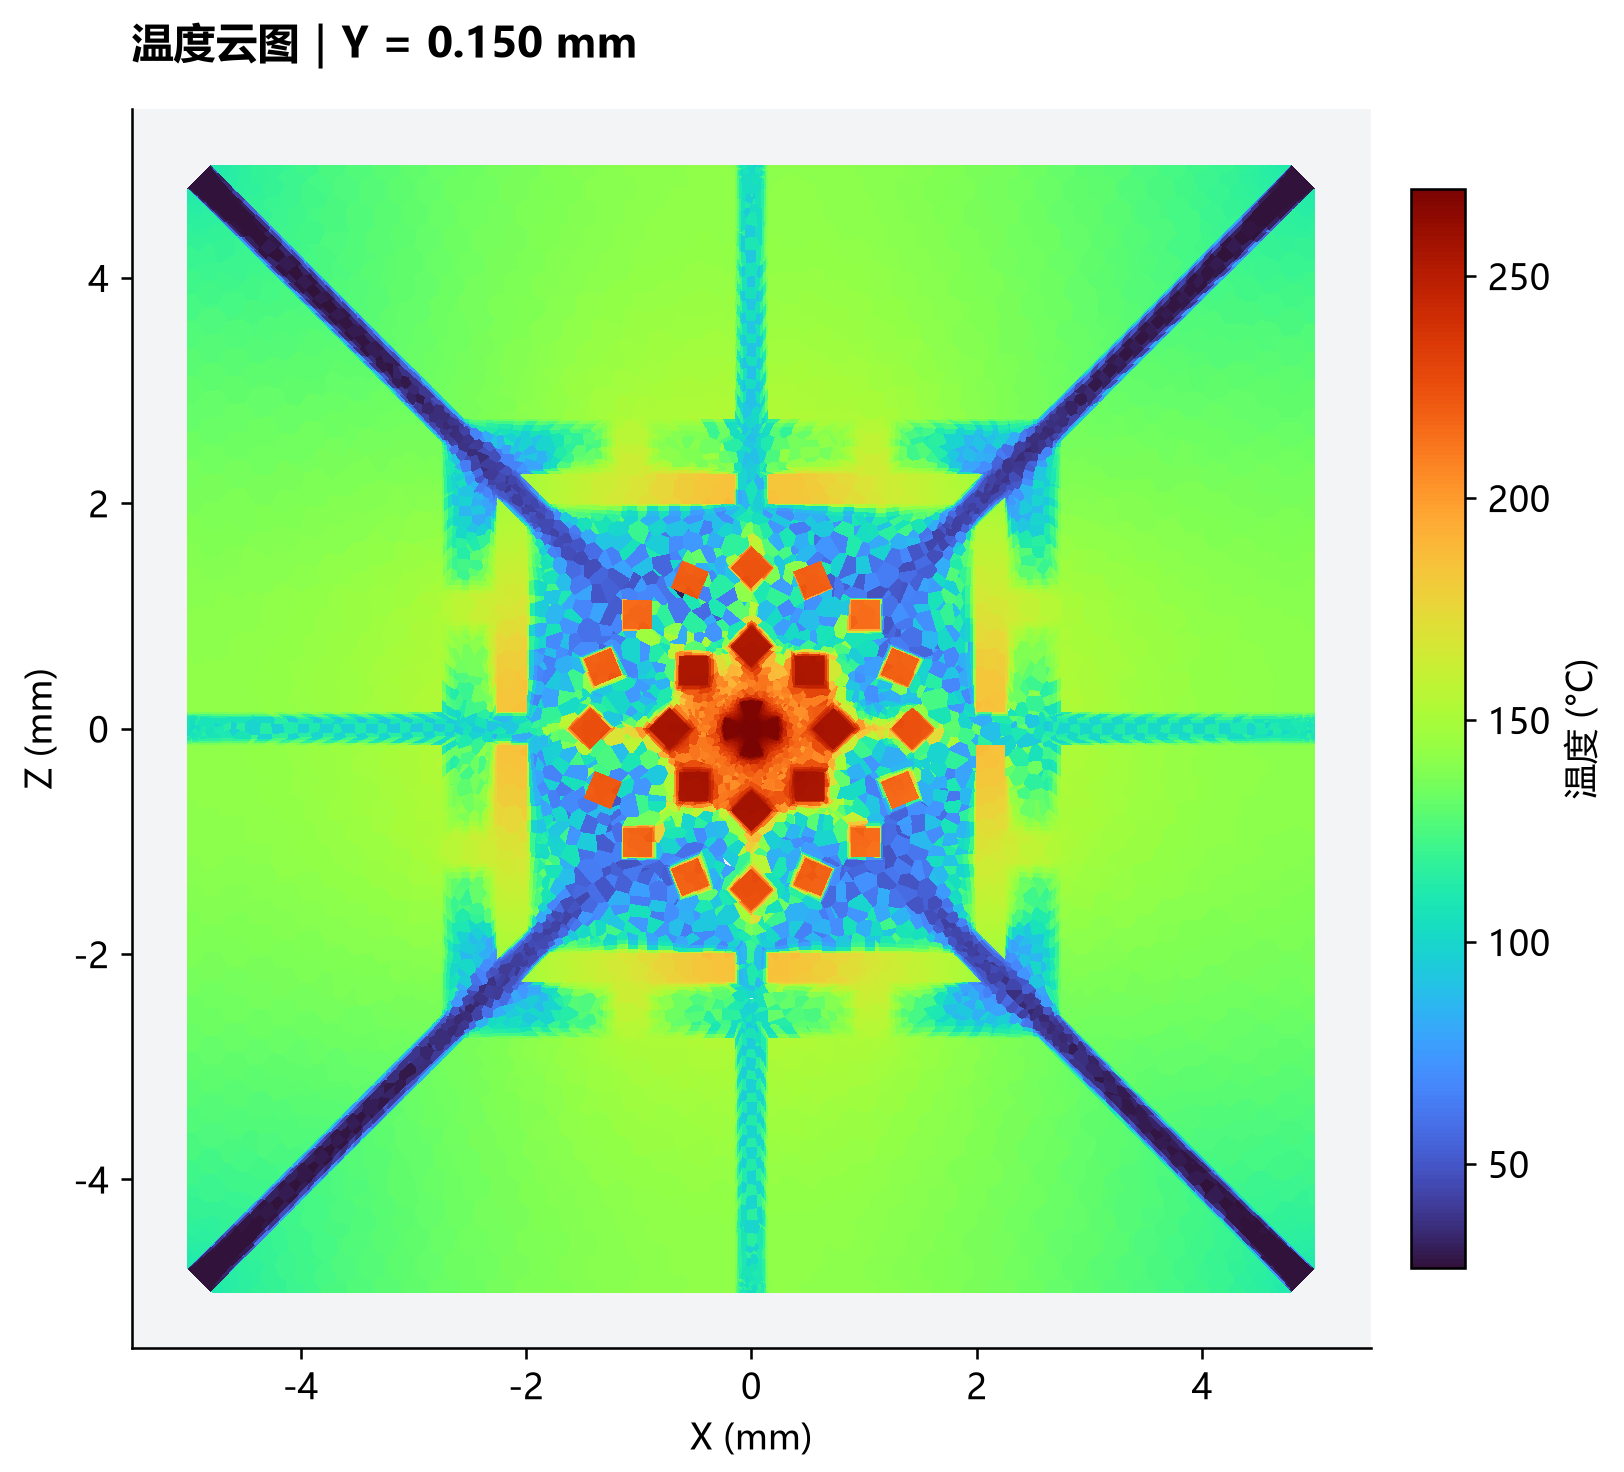
\includegraphics[width=\linewidth]{figs/midterm_monthly1_01_temperature_midplane.png}
\caption{水侧温度}\end{subfigure}\hfill
\begin{subfigure}{.235\linewidth}\centering
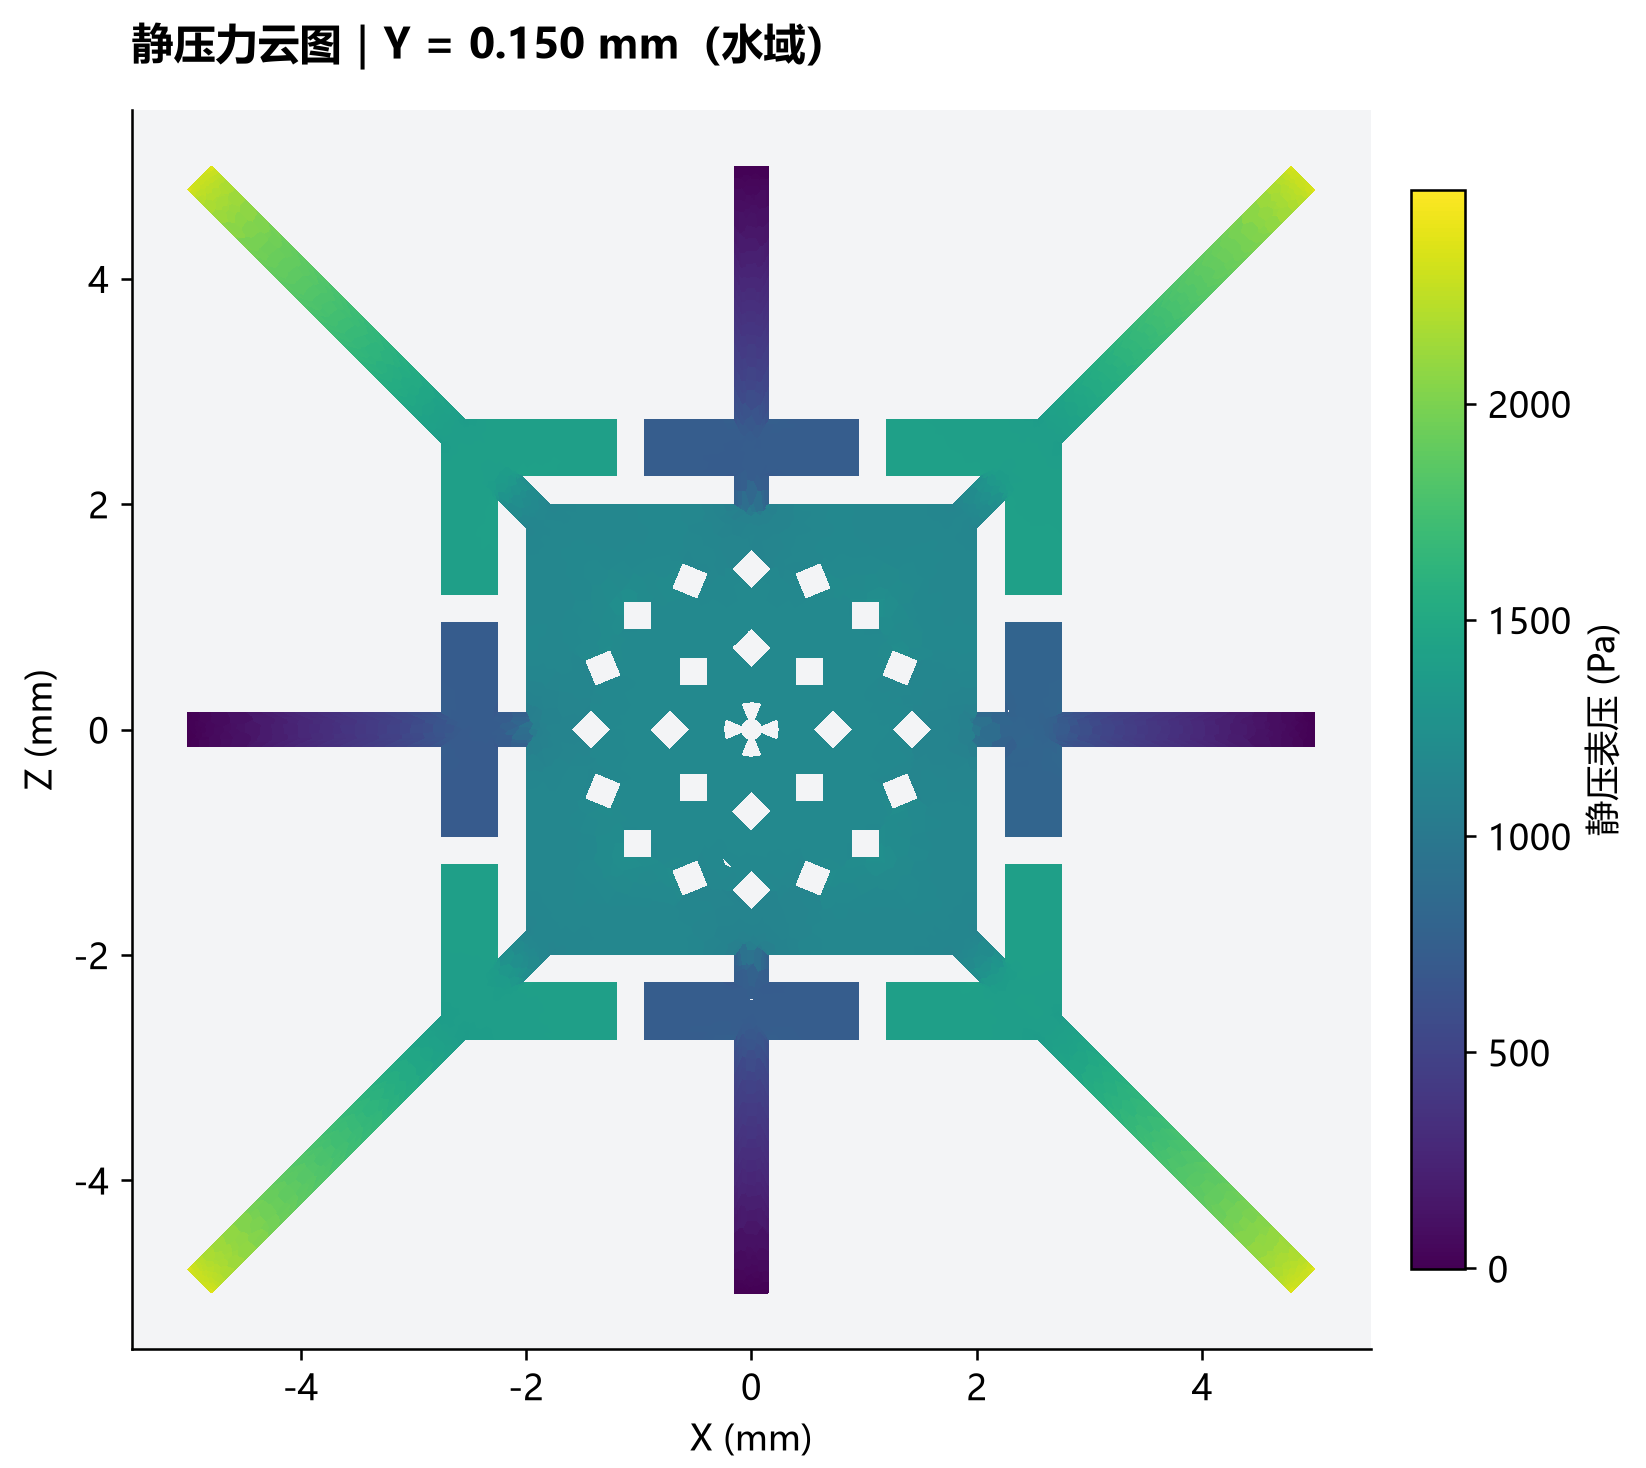
\includegraphics[width=\linewidth]{figs/midterm_monthly1_02_pressure_midplane.png}
\caption{水侧表压}\end{subfigure}\hfill
\begin{subfigure}{.235\linewidth}\centering
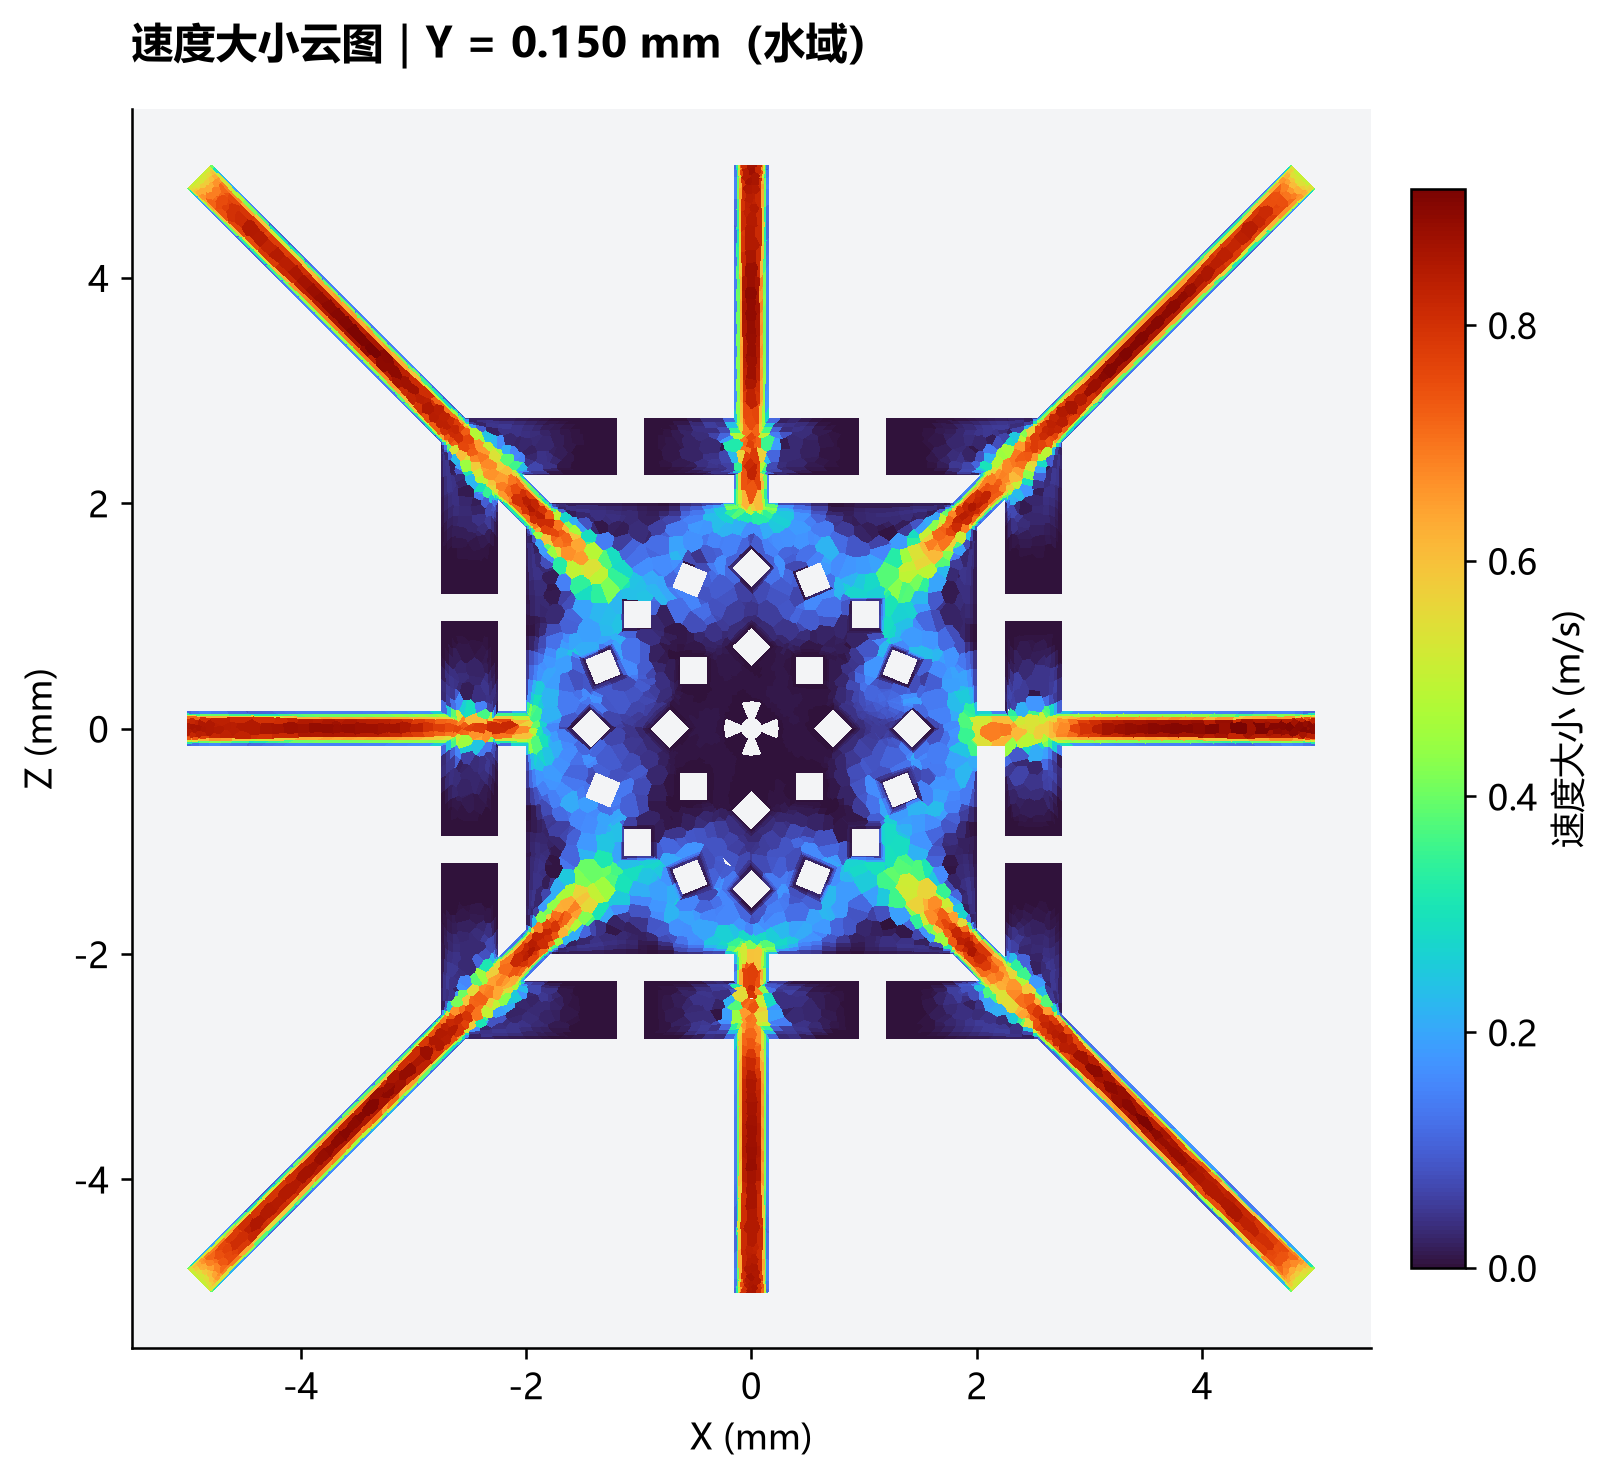
\includegraphics[width=\linewidth]{figs/midterm_monthly1_03_speed_midplane.png}
\caption{水侧速度大小}\end{subfigure}\hfill
\begin{subfigure}{.235\linewidth}\centering
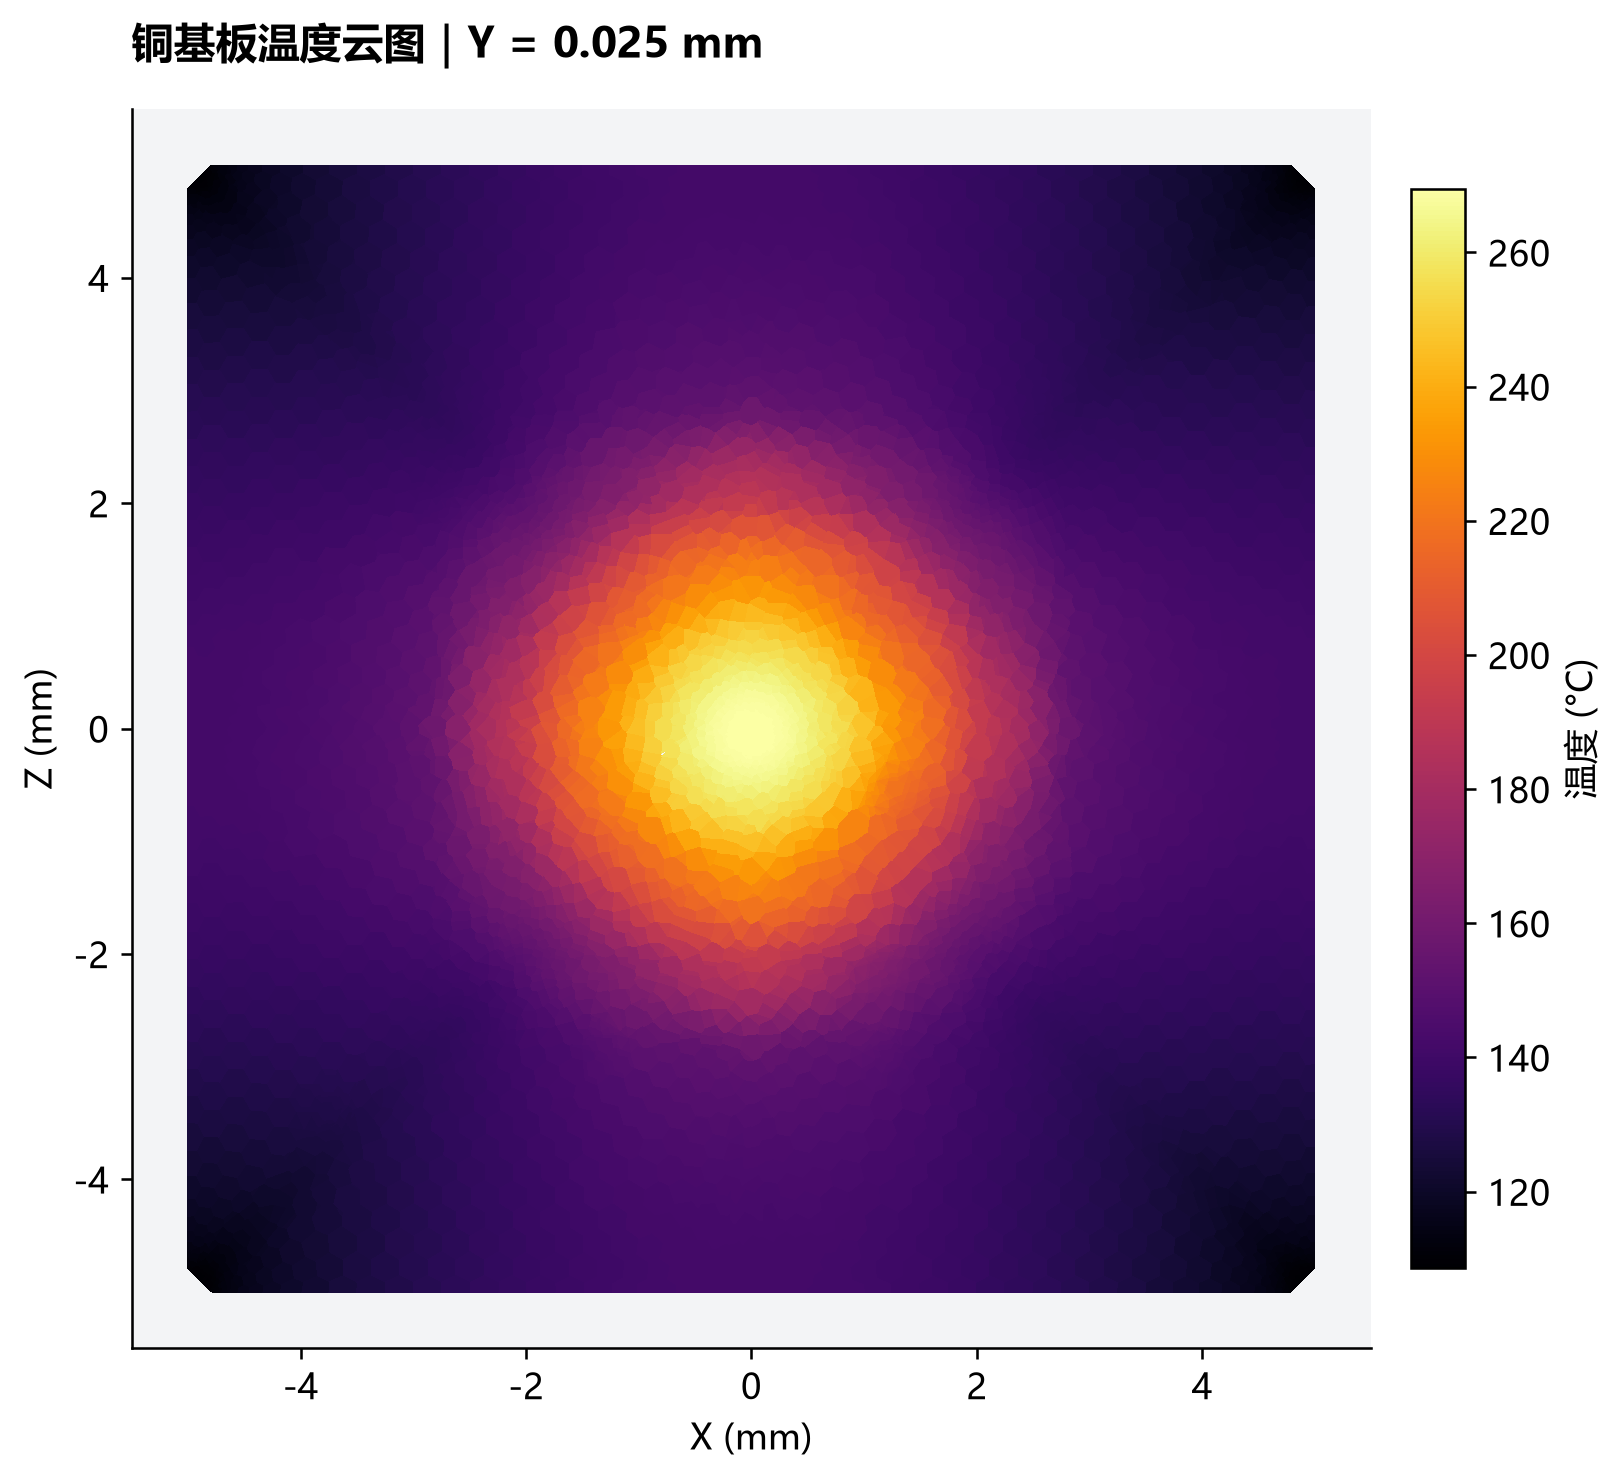
\includegraphics[width=\linewidth]{figs/midterm_monthly1_04_copper_base_temperature.png}
\caption{铜基板温度}\end{subfigure}

\vspace{4pt}
{\small\heiti 六边形微通道}\par\vspace{1pt}
\begin{subfigure}{.235\linewidth}\centering
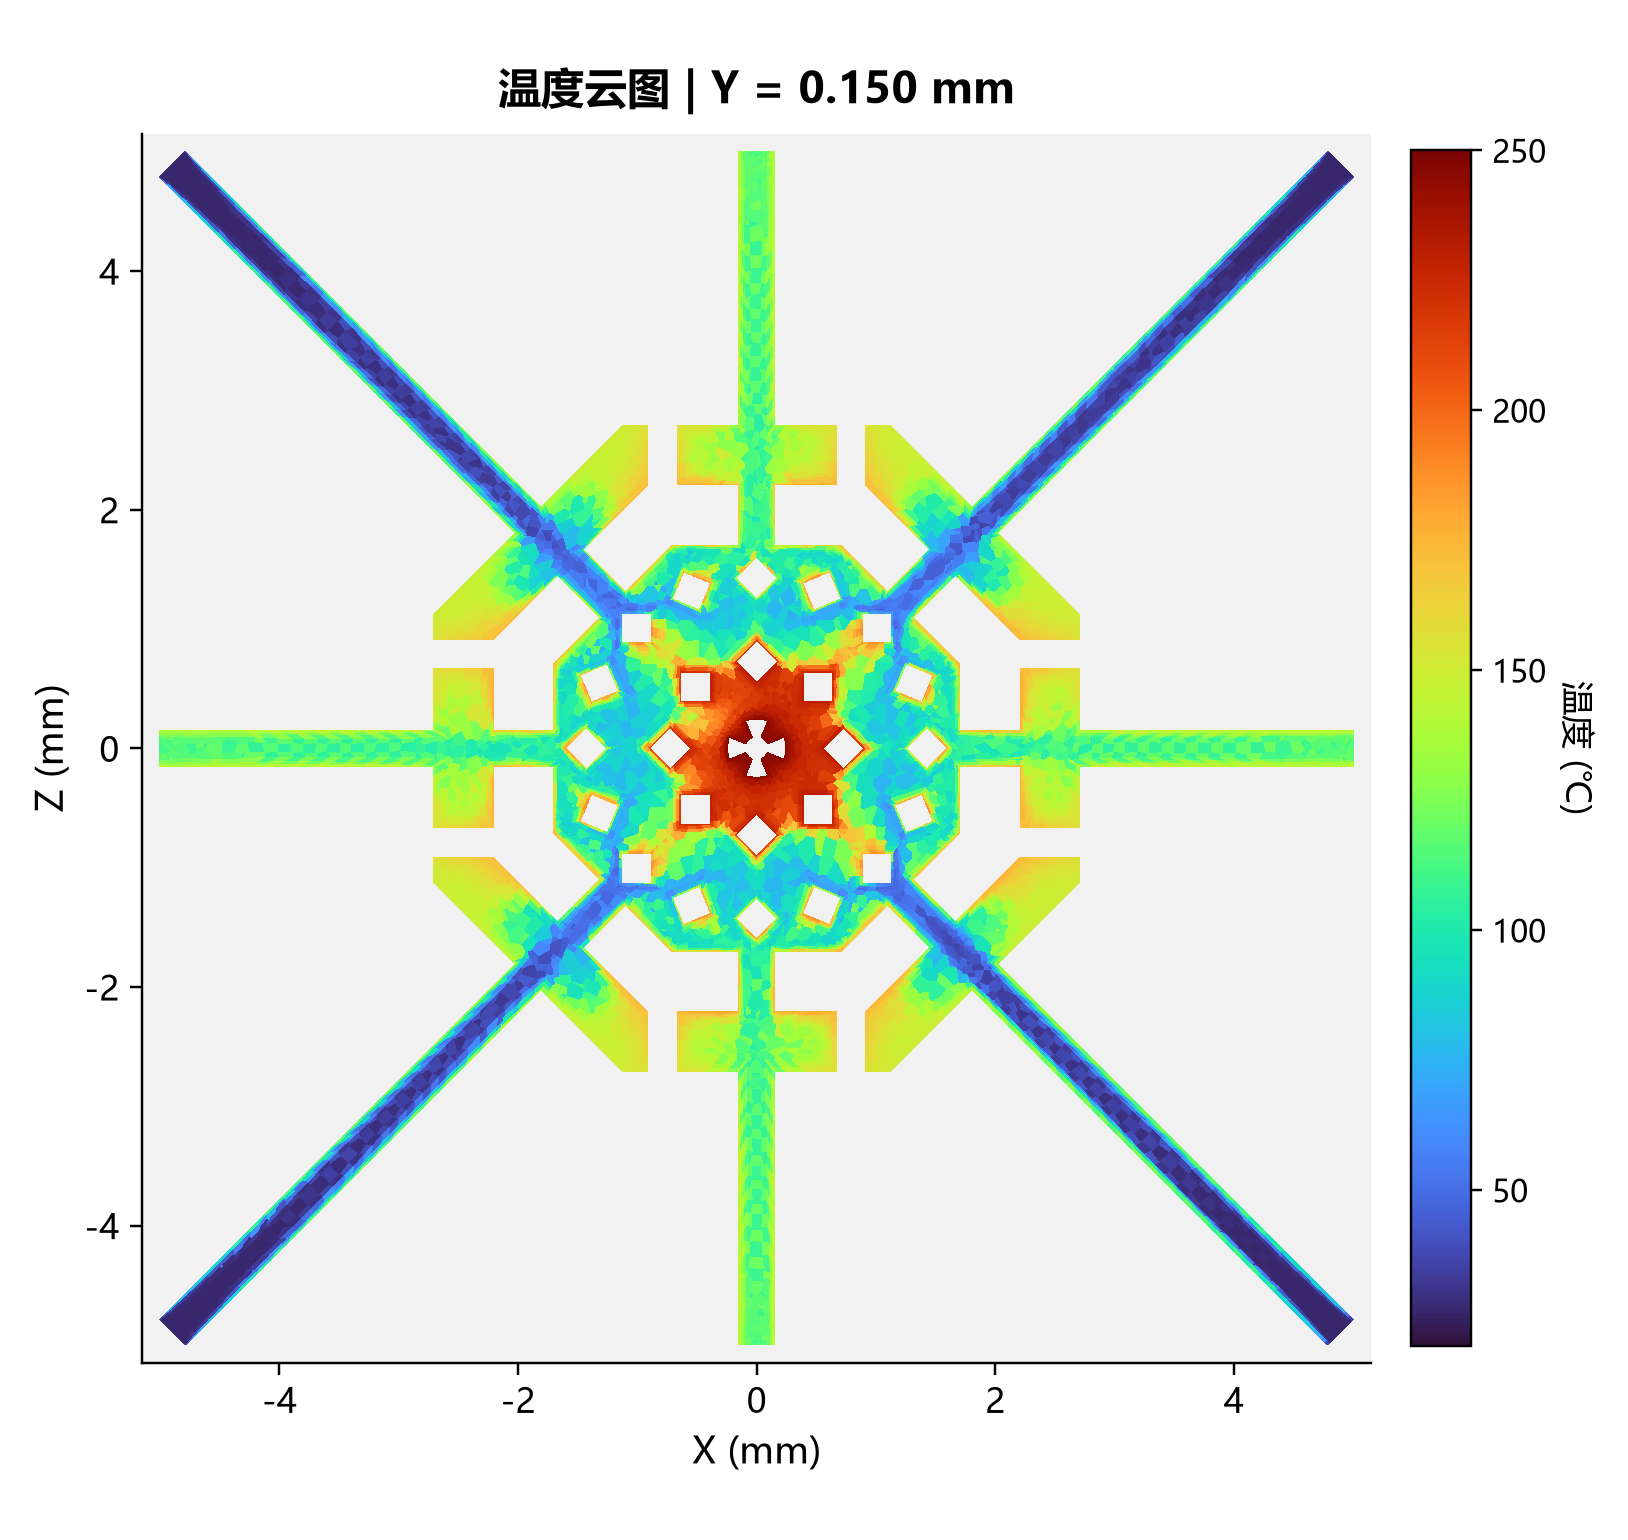
\includegraphics[width=\linewidth]{figs/midterm_monthly1_05_temperature_midplane.png}\end{subfigure}\hfill
\begin{subfigure}{.235\linewidth}\centering
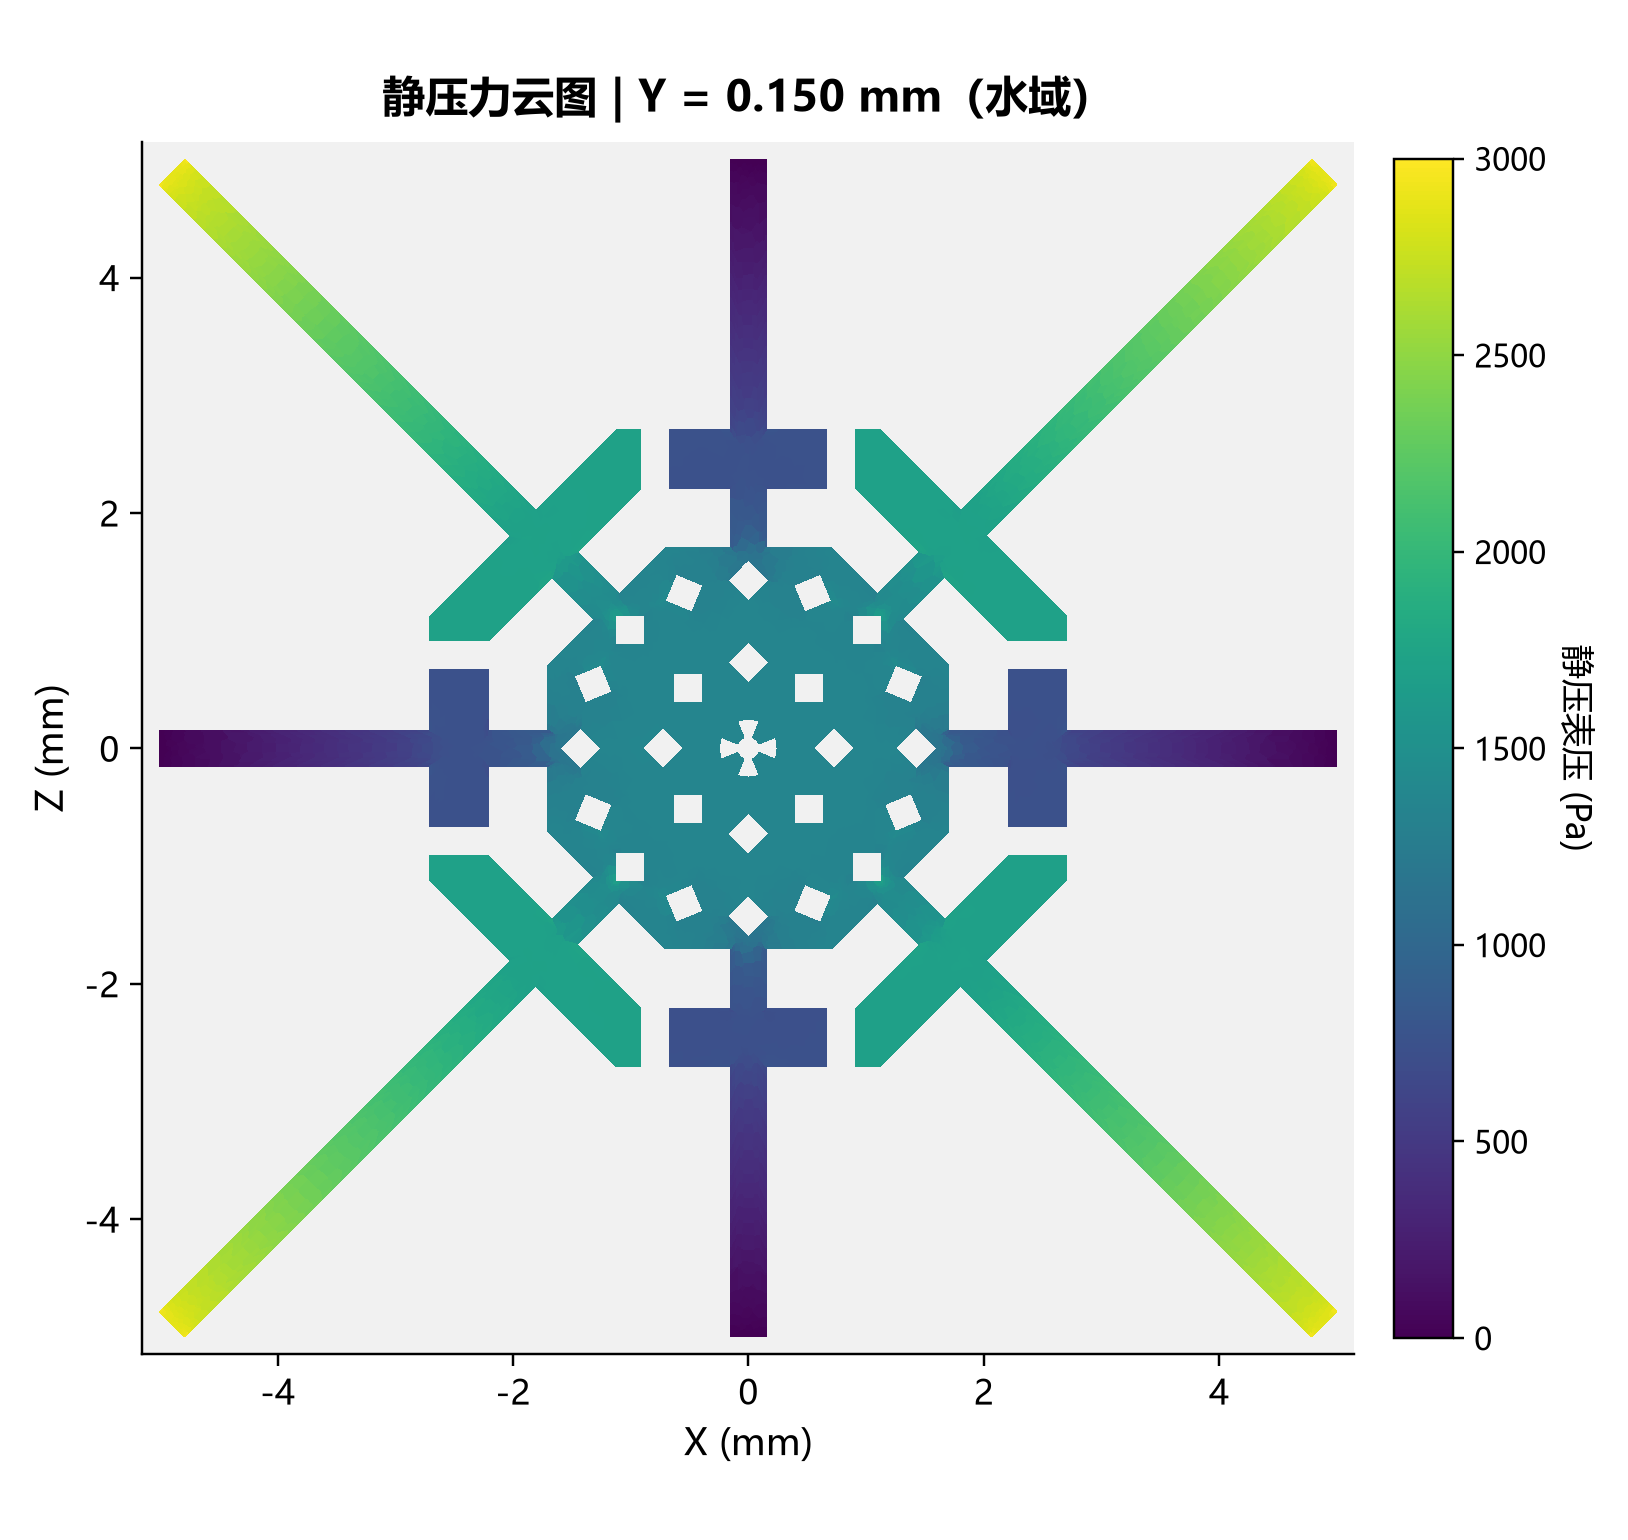
\includegraphics[width=\linewidth]{figs/midterm_monthly1_06_pressure_midplane.png}\end{subfigure}\hfill
\begin{subfigure}{.235\linewidth}\centering
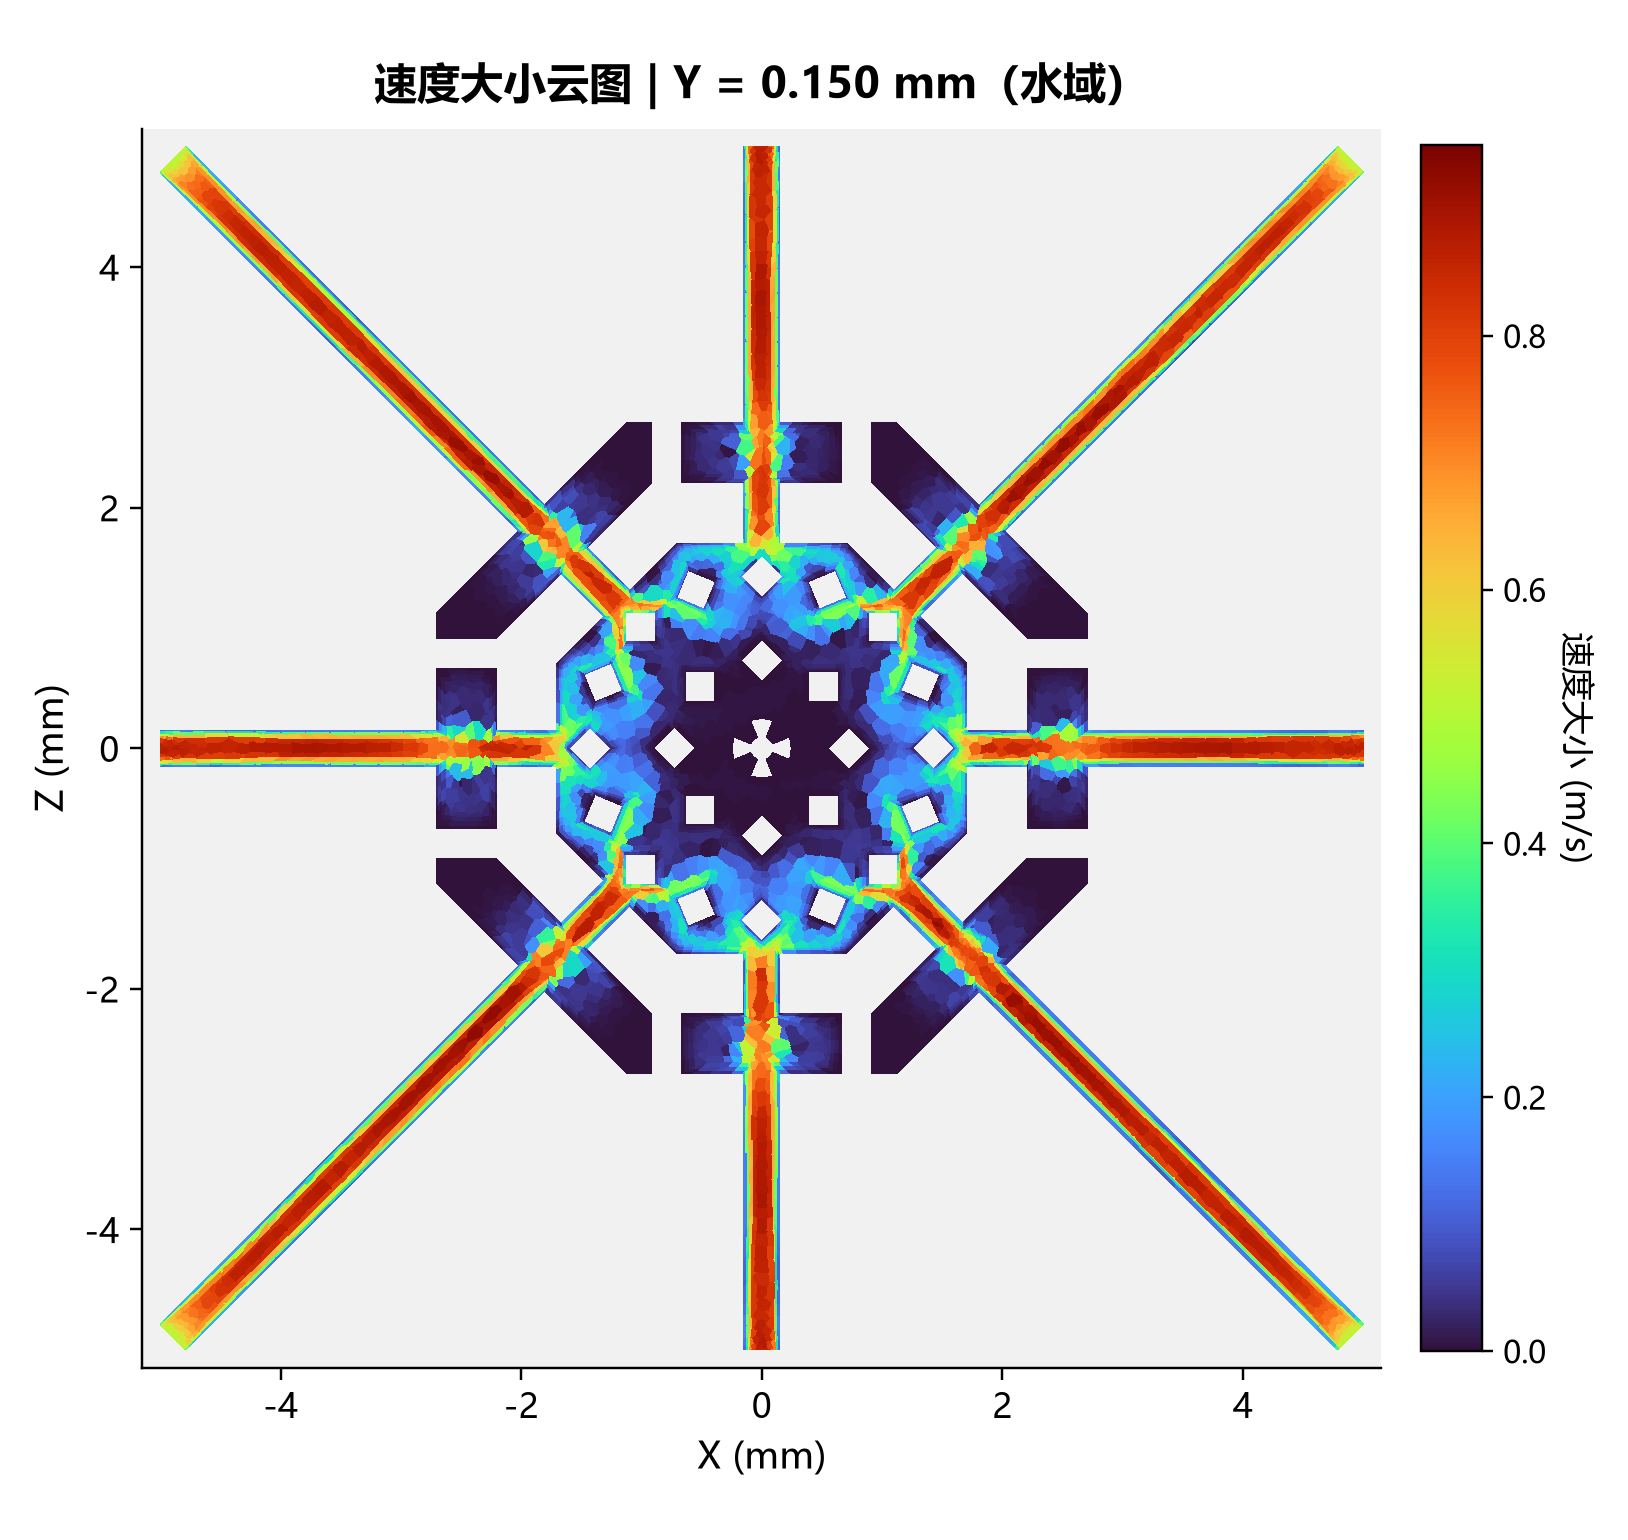
\includegraphics[width=\linewidth]{figs/midterm_monthly1_07_speed_midplane.png}\end{subfigure}\hfill
\begin{subfigure}{.235\linewidth}\centering
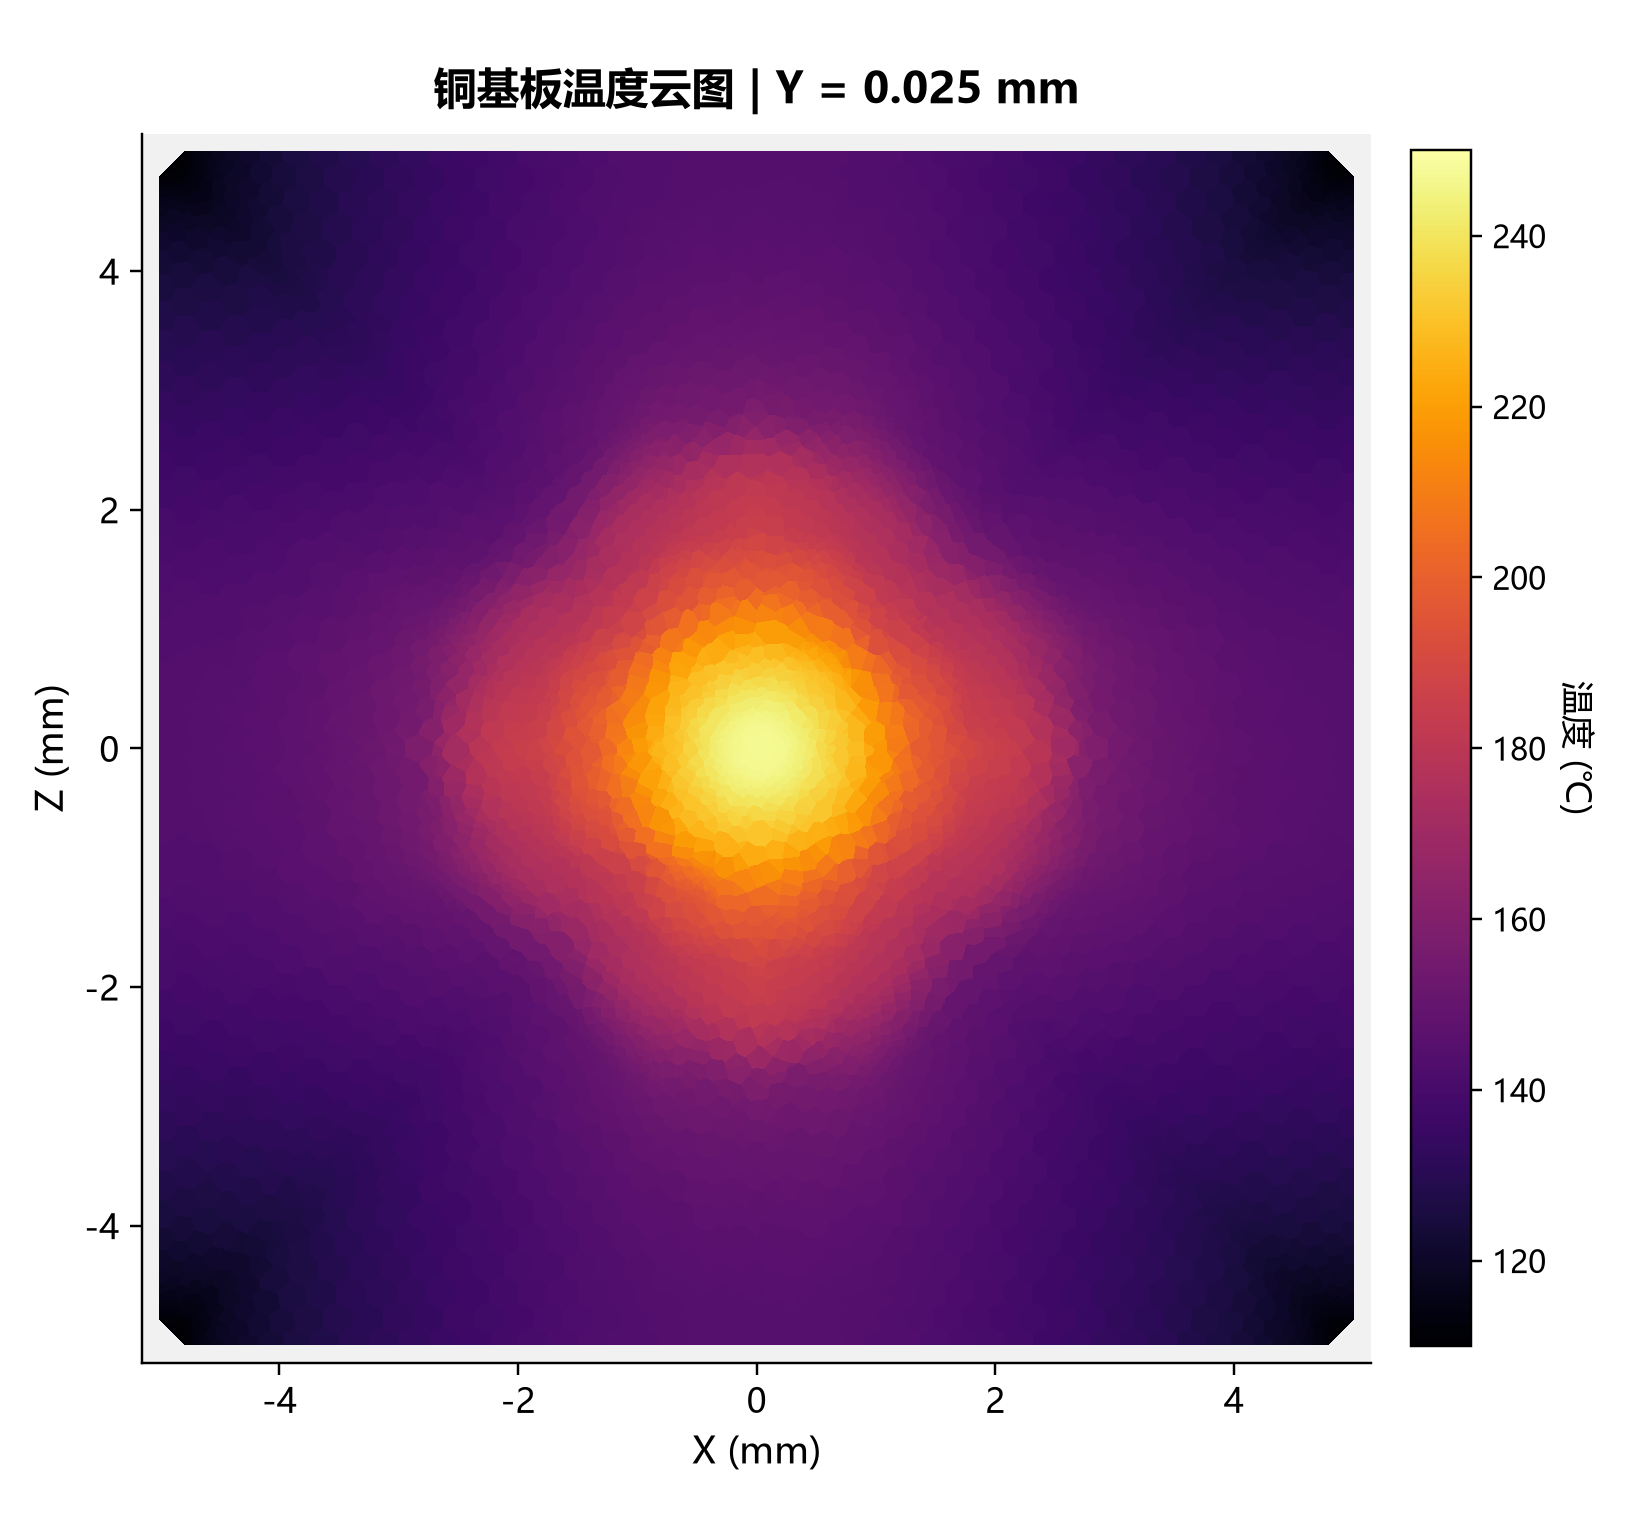
\includegraphics[width=\linewidth]{figs/midterm_monthly1_08_copper_base_temperature.png}\end{subfigure}

\vspace{4pt}
{\small\heiti 圆形微通道}\par\vspace{1pt}
\begin{subfigure}{.235\linewidth}\centering
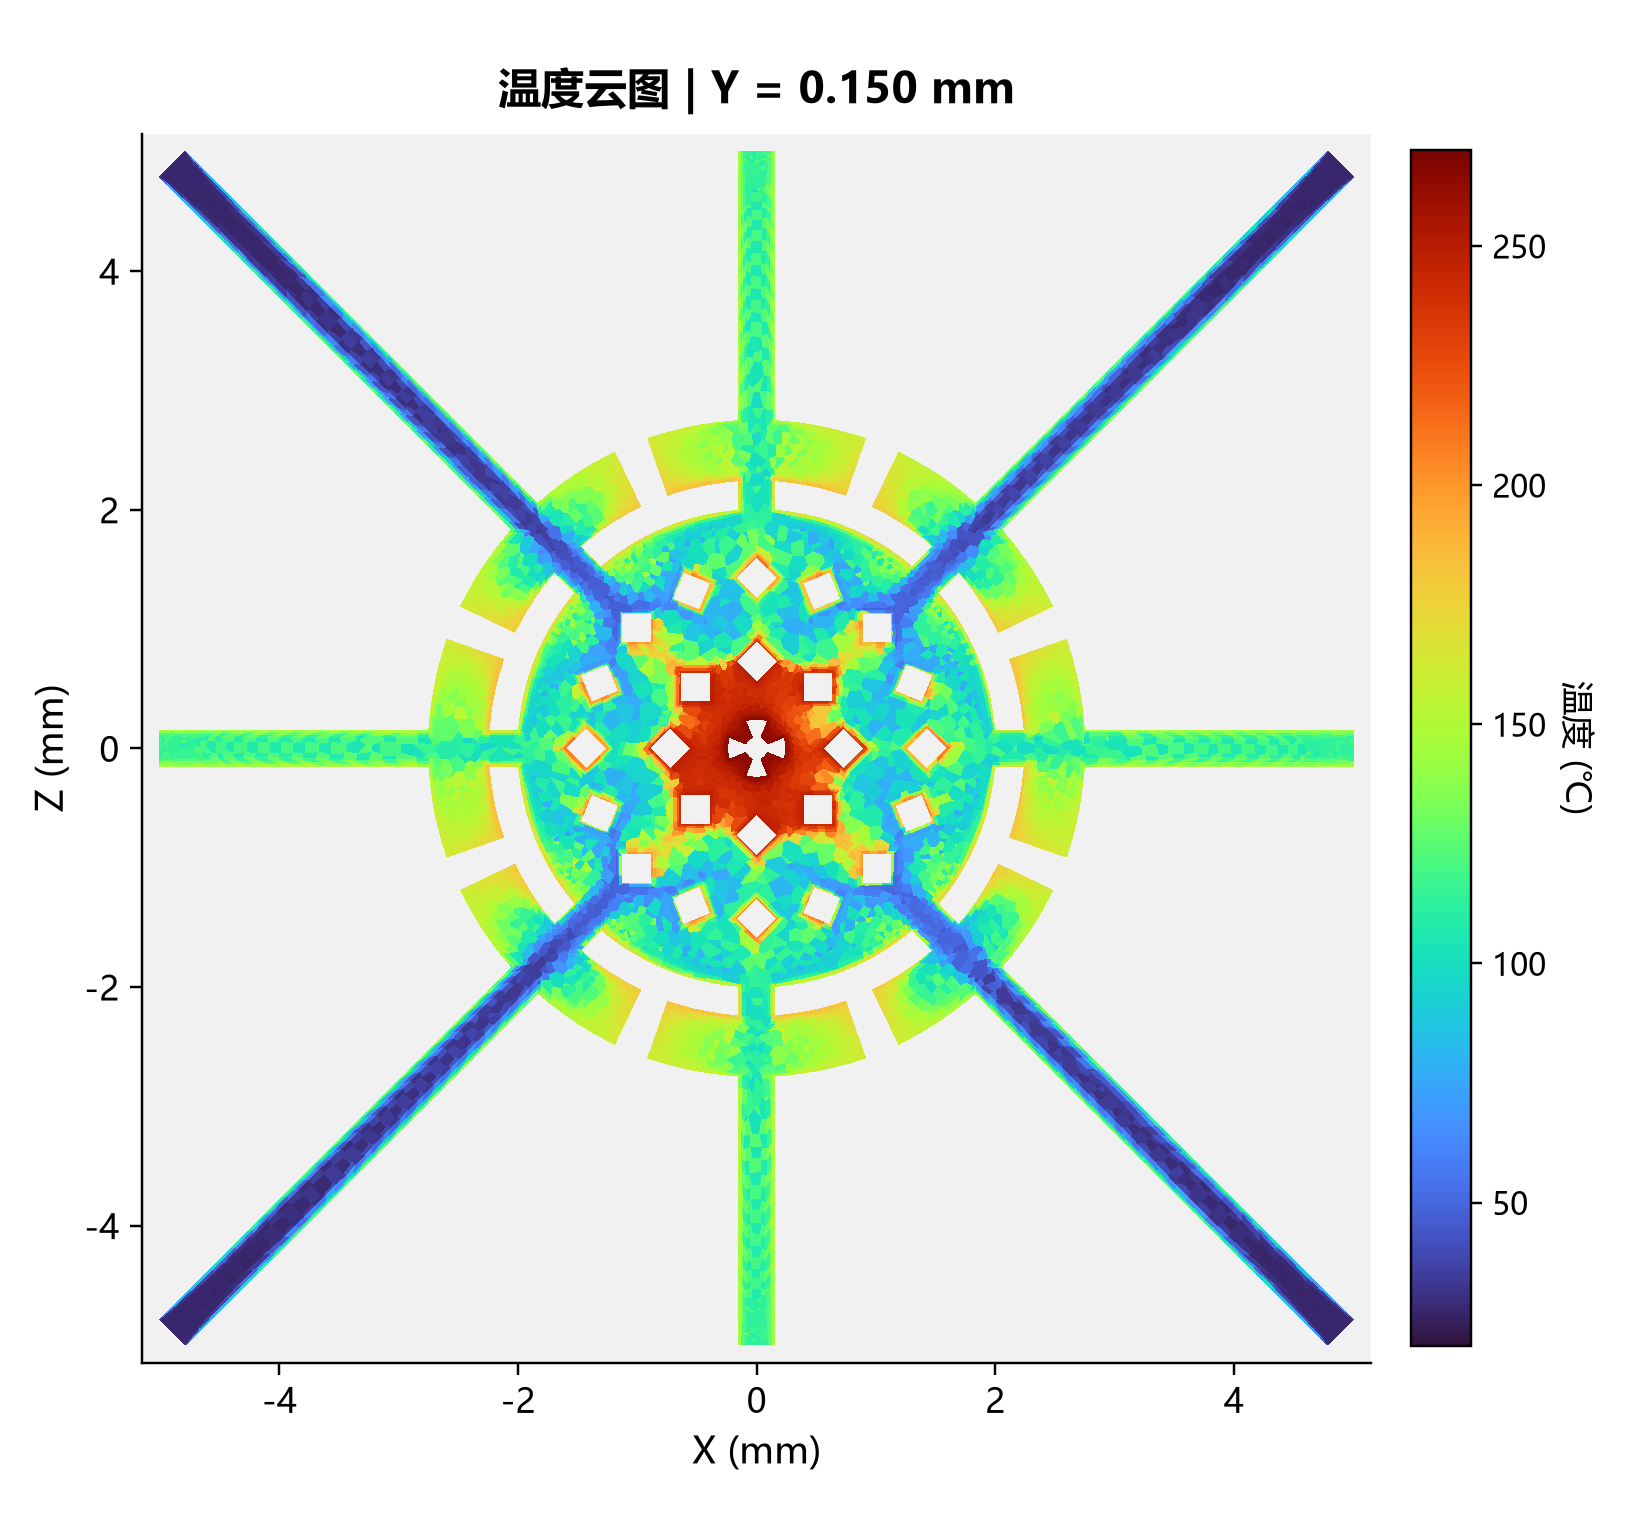
\includegraphics[width=\linewidth]{figs/midterm_monthly1_09_temperature_midplane.png}\end{subfigure}\hfill
\begin{subfigure}{.235\linewidth}\centering
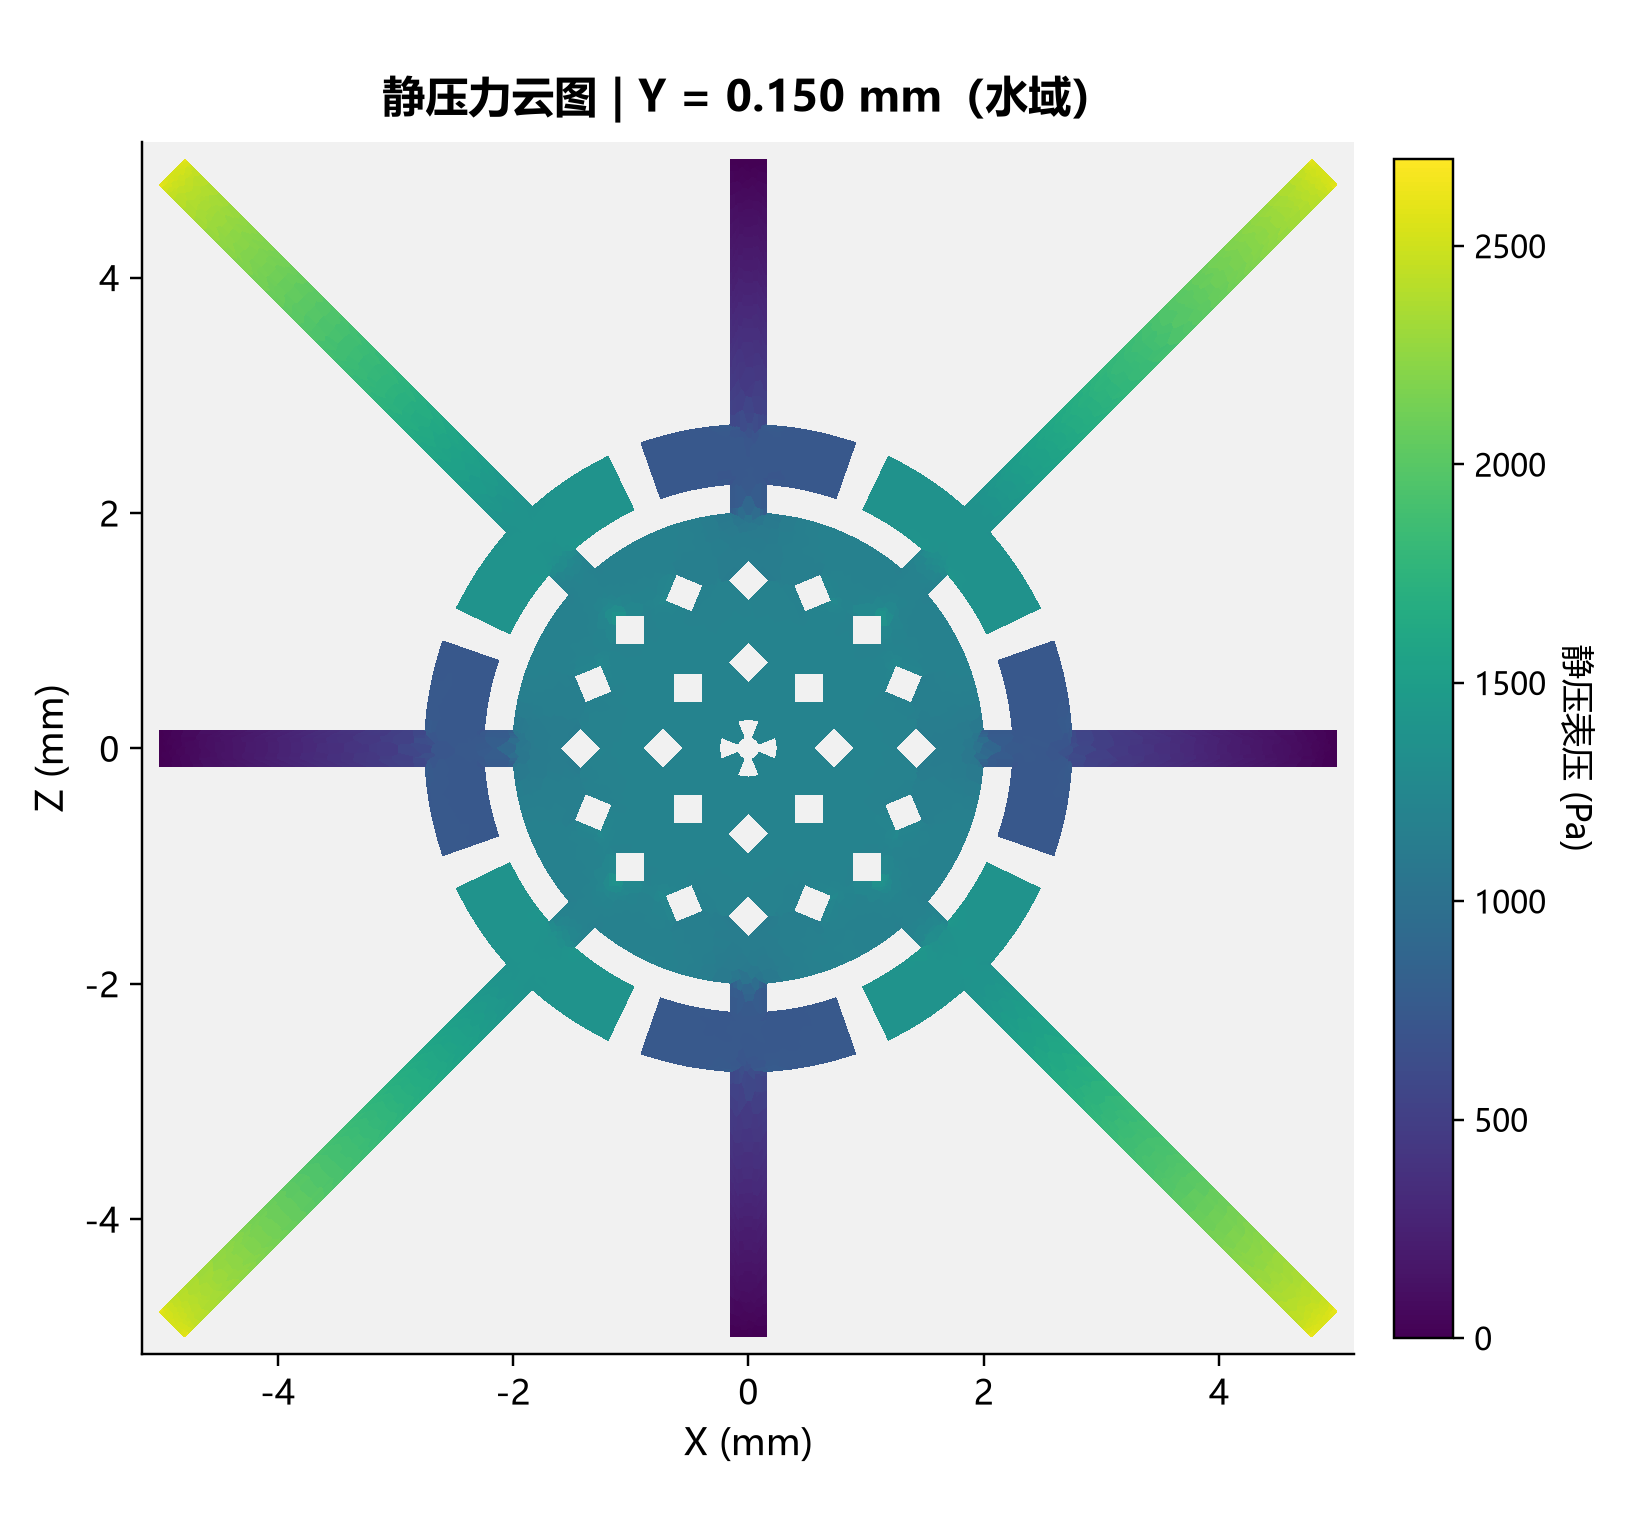
\includegraphics[width=\linewidth]{figs/midterm_monthly1_10_pressure_midplane.png}\end{subfigure}\hfill
\begin{subfigure}{.235\linewidth}\centering
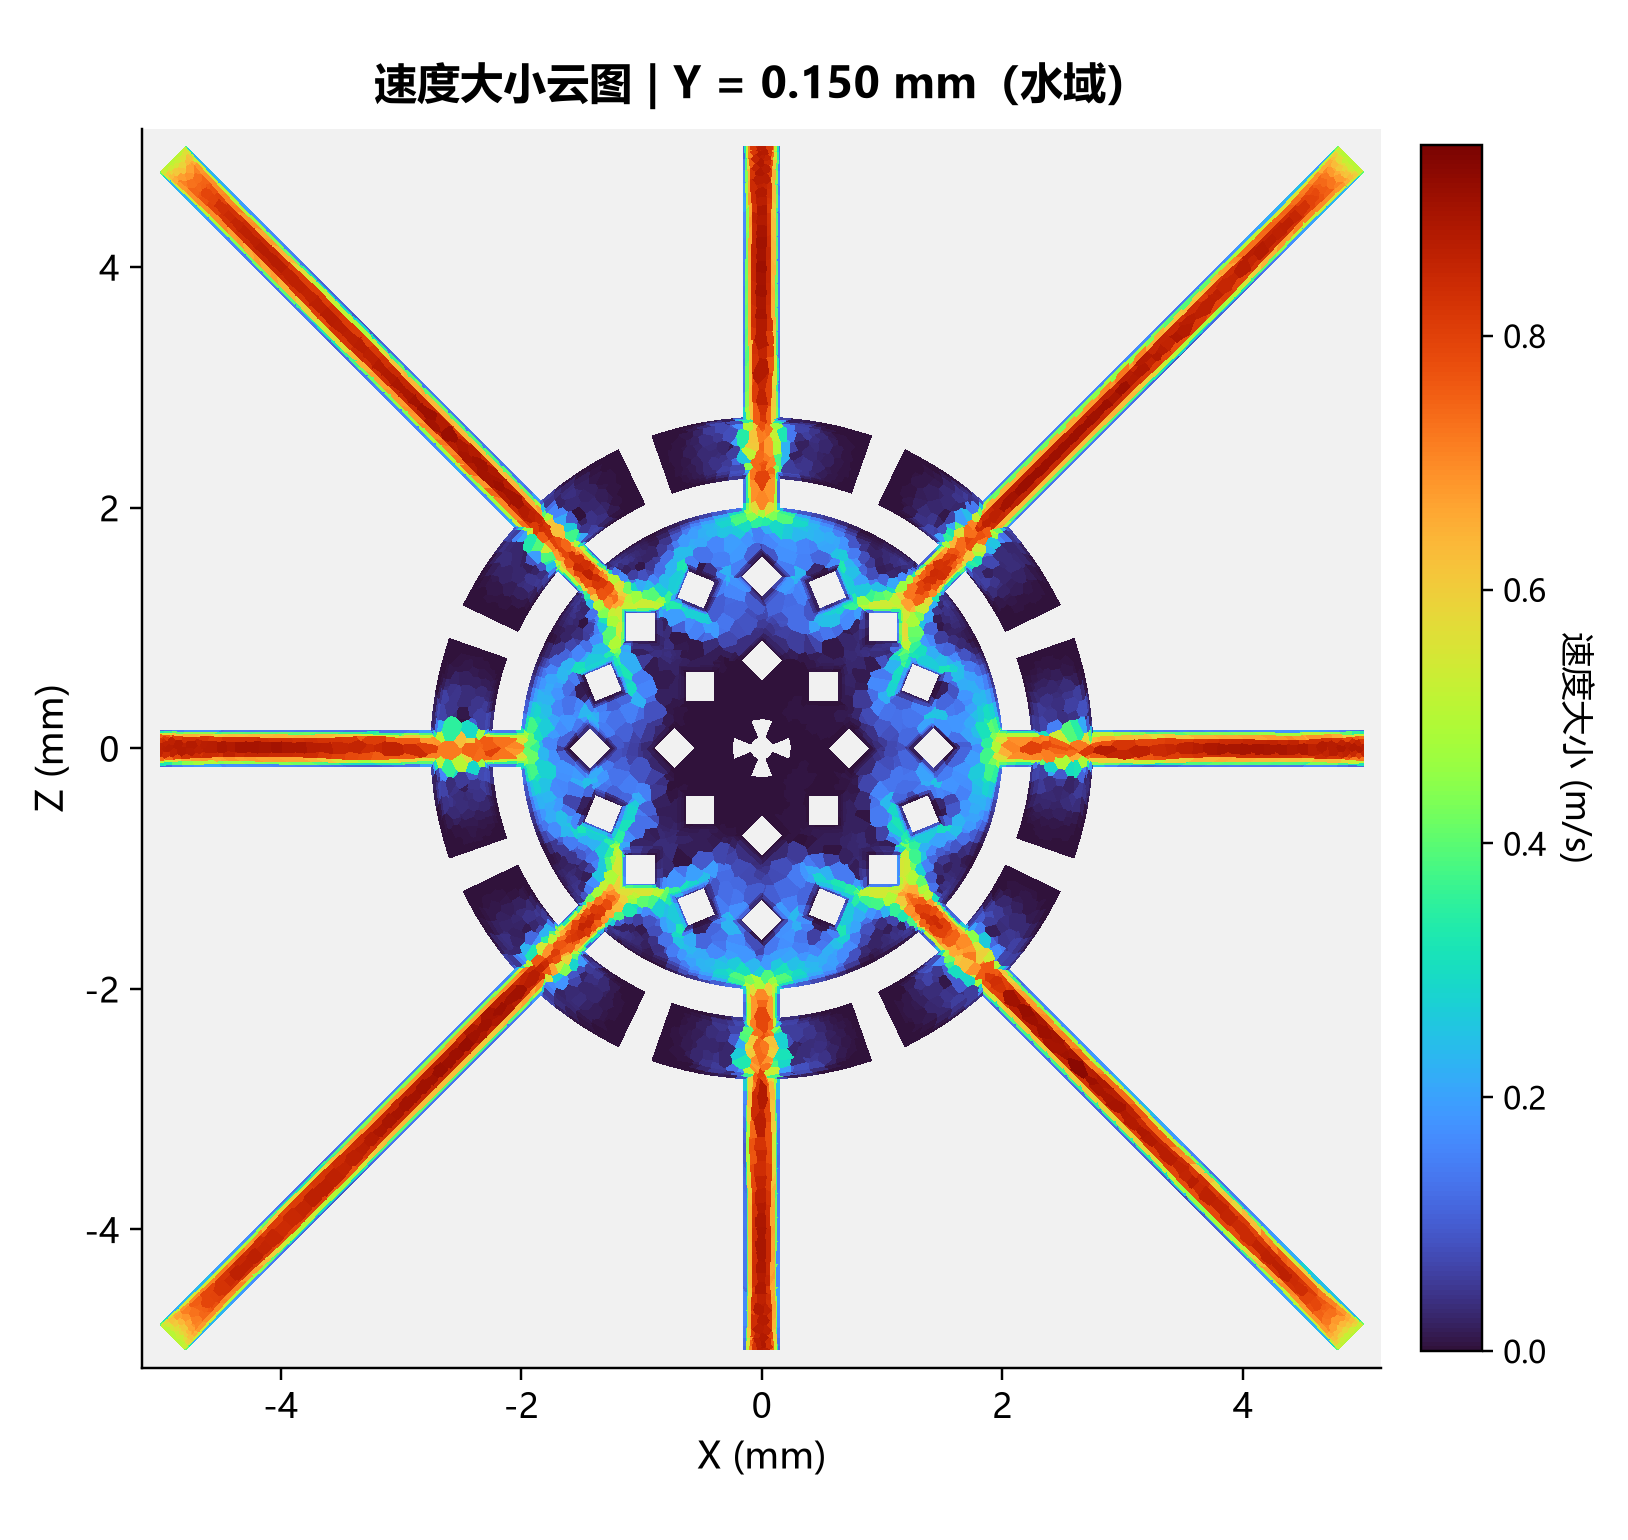
\includegraphics[width=\linewidth]{figs/midterm_monthly1_11_speed_midplane.png}\end{subfigure}\hfill
\begin{subfigure}{.235\linewidth}\centering
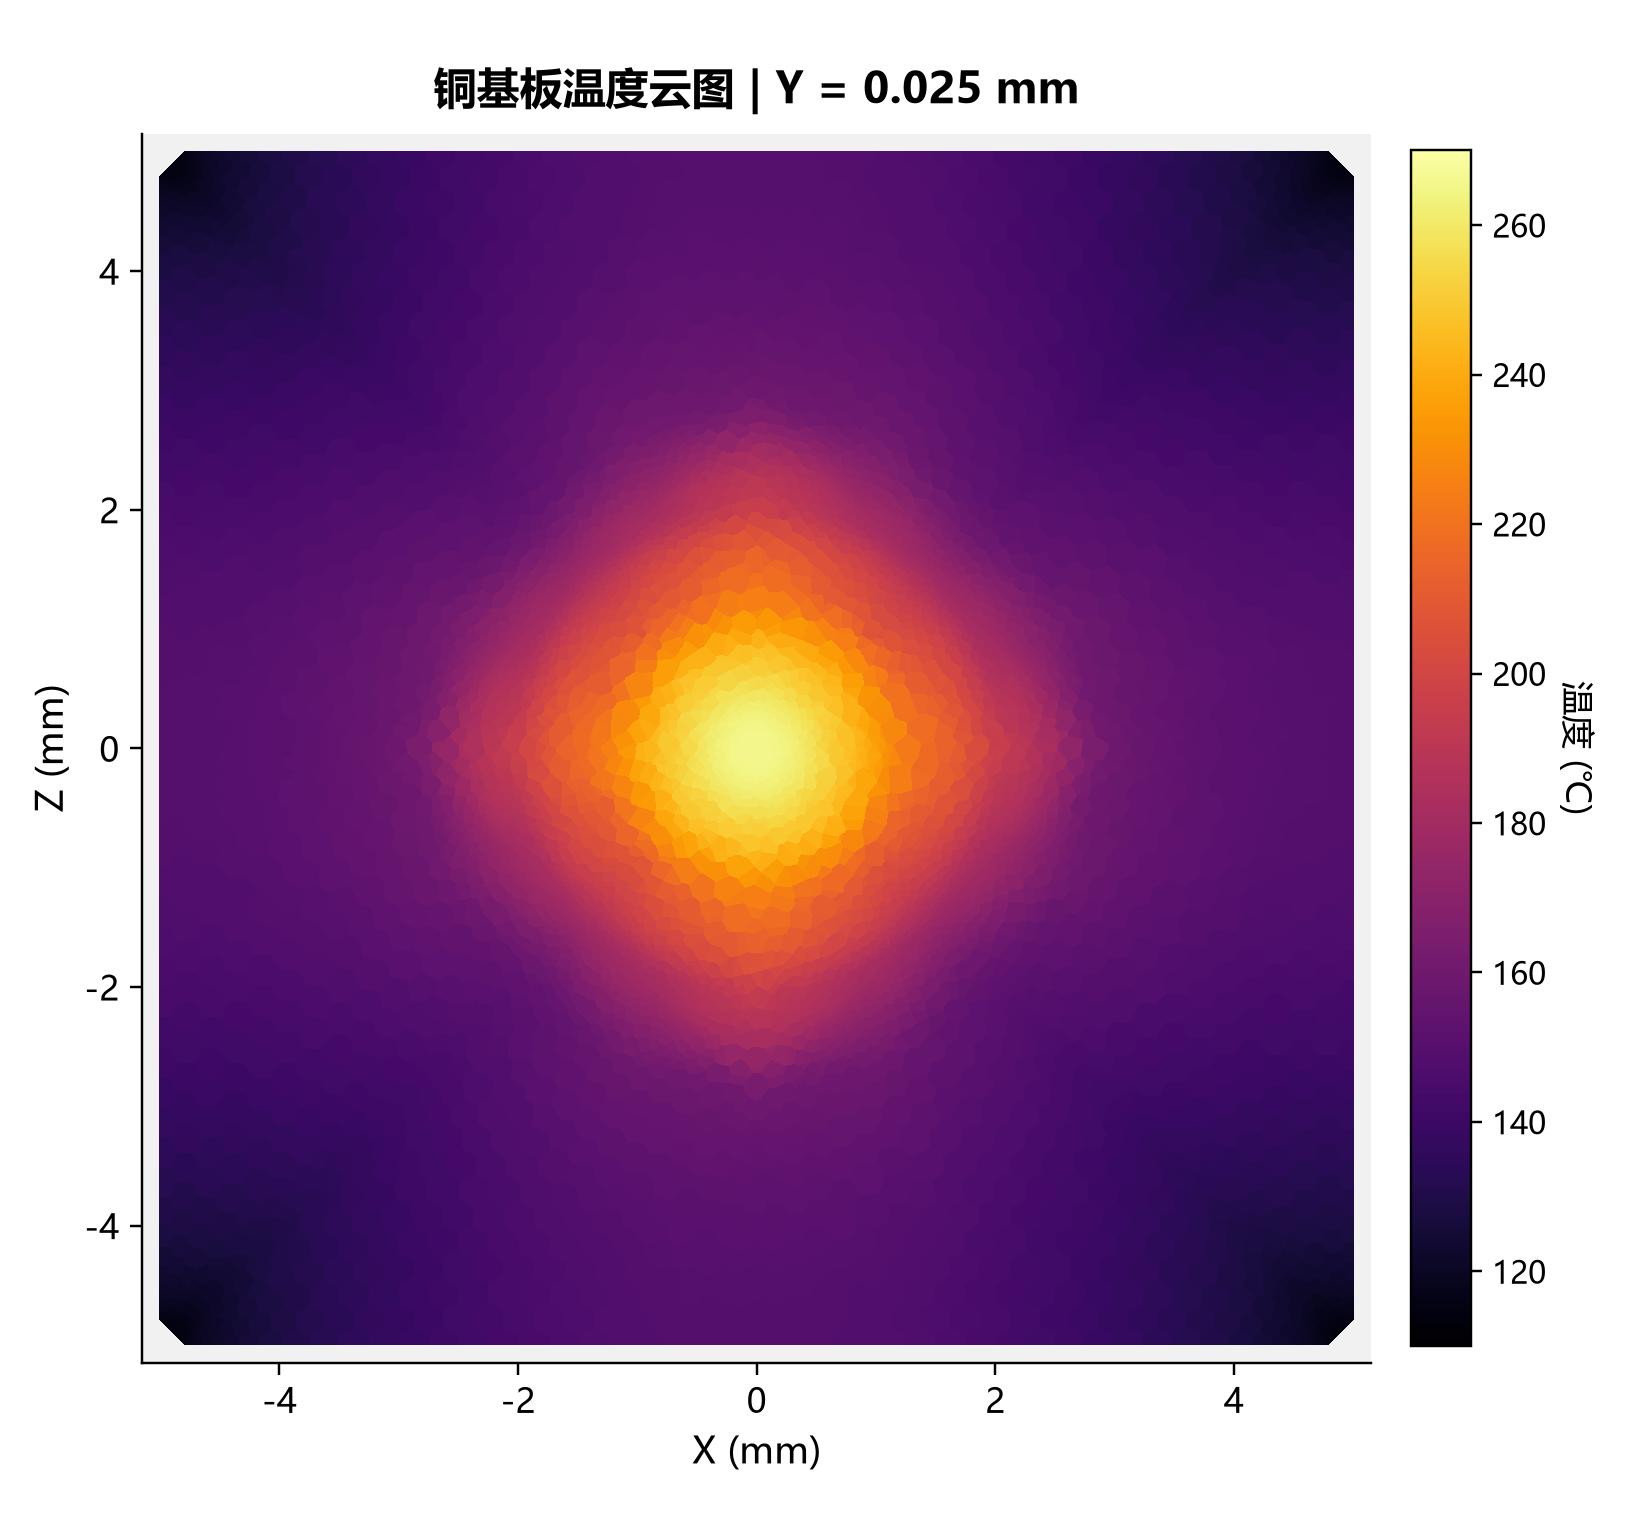
\includegraphics[width=\linewidth]{figs/midterm_monthly1_12_copper_base_temperature.png}\end{subfigure}
\caption{三组流道的复现云图：自上而下为方形、六边形与圆形微通道，自左至右为水侧温度、水侧表压、水侧速度大小与铜基板温度。水侧取 $Y=0.150$ mm，铜基板取 $Y=0.025$ mm；保留各图原色标，不能由颜色直接比较不同工况。}
\label{fig:repro}
\end{figure}
\subsubsection{网格诊断结果}
本报告提取了 NACA2416\_v3 在 $0.2\,\mathrm{s}$ 的七档已有结果，见表\ref{tab:04}。其中“平均温度”沿用原数据的全域单元算术平均，并非体积加权、受热面平均或流体混合温度；“最高温度”为全域最大值；压降为进出口面积平均静压差。该数据只能按原定义解释，不作为连接结构的优势数据。图\ref{fig:08}给出统一平面的实际面网格，图\ref{fig:09}给出已有响应曲线。
\begin{table}[!htbp]
\centering\small
\caption{NACA2416\_v3七档网格在0.2 s的已有结果}\label{tab:04}
\begin{tabularx}{\linewidth}{lYYY}
\toprule
\rowcolor{ydzjlight} 单元数 & 平均温度/K & 最高温度/K & 静压差/Pa \\
\midrule
260169 & 304.668393 & 344.675487 & 2505.203605 \\
575129 & 304.411275 & 345.265735 & 2389.274100 \\
1073583 & 303.944909 & 345.153612 & 2440.765641 \\
1524876 & 305.093298 & 346.048803 & 2389.938449 \\
2943269 & 304.373551 & 345.964030 & 2355.838476 \\
3235081 & 304.300924 & 345.983833 & 2348.320348 \\
4610769 & 305.985989 & 346.618797 & 2448.714104 \\
\bottomrule
\end{tabularx}
\par\smallskip\begin{minipage}{\linewidth}\footnotesize 温度为全域单元算术平均及全域最高值，静压为进出口面积平均；非受热面指标。最细档有不同时间步历史，未通过全序列1\%联合判据。来源：配套源码目录内 evidence/mesh\_results\_02s.csv。—。\end{minipage}
\end{table}


\begin{figure}[!htbp]\centering
\begin{subfigure}{0.49\linewidth}\centering
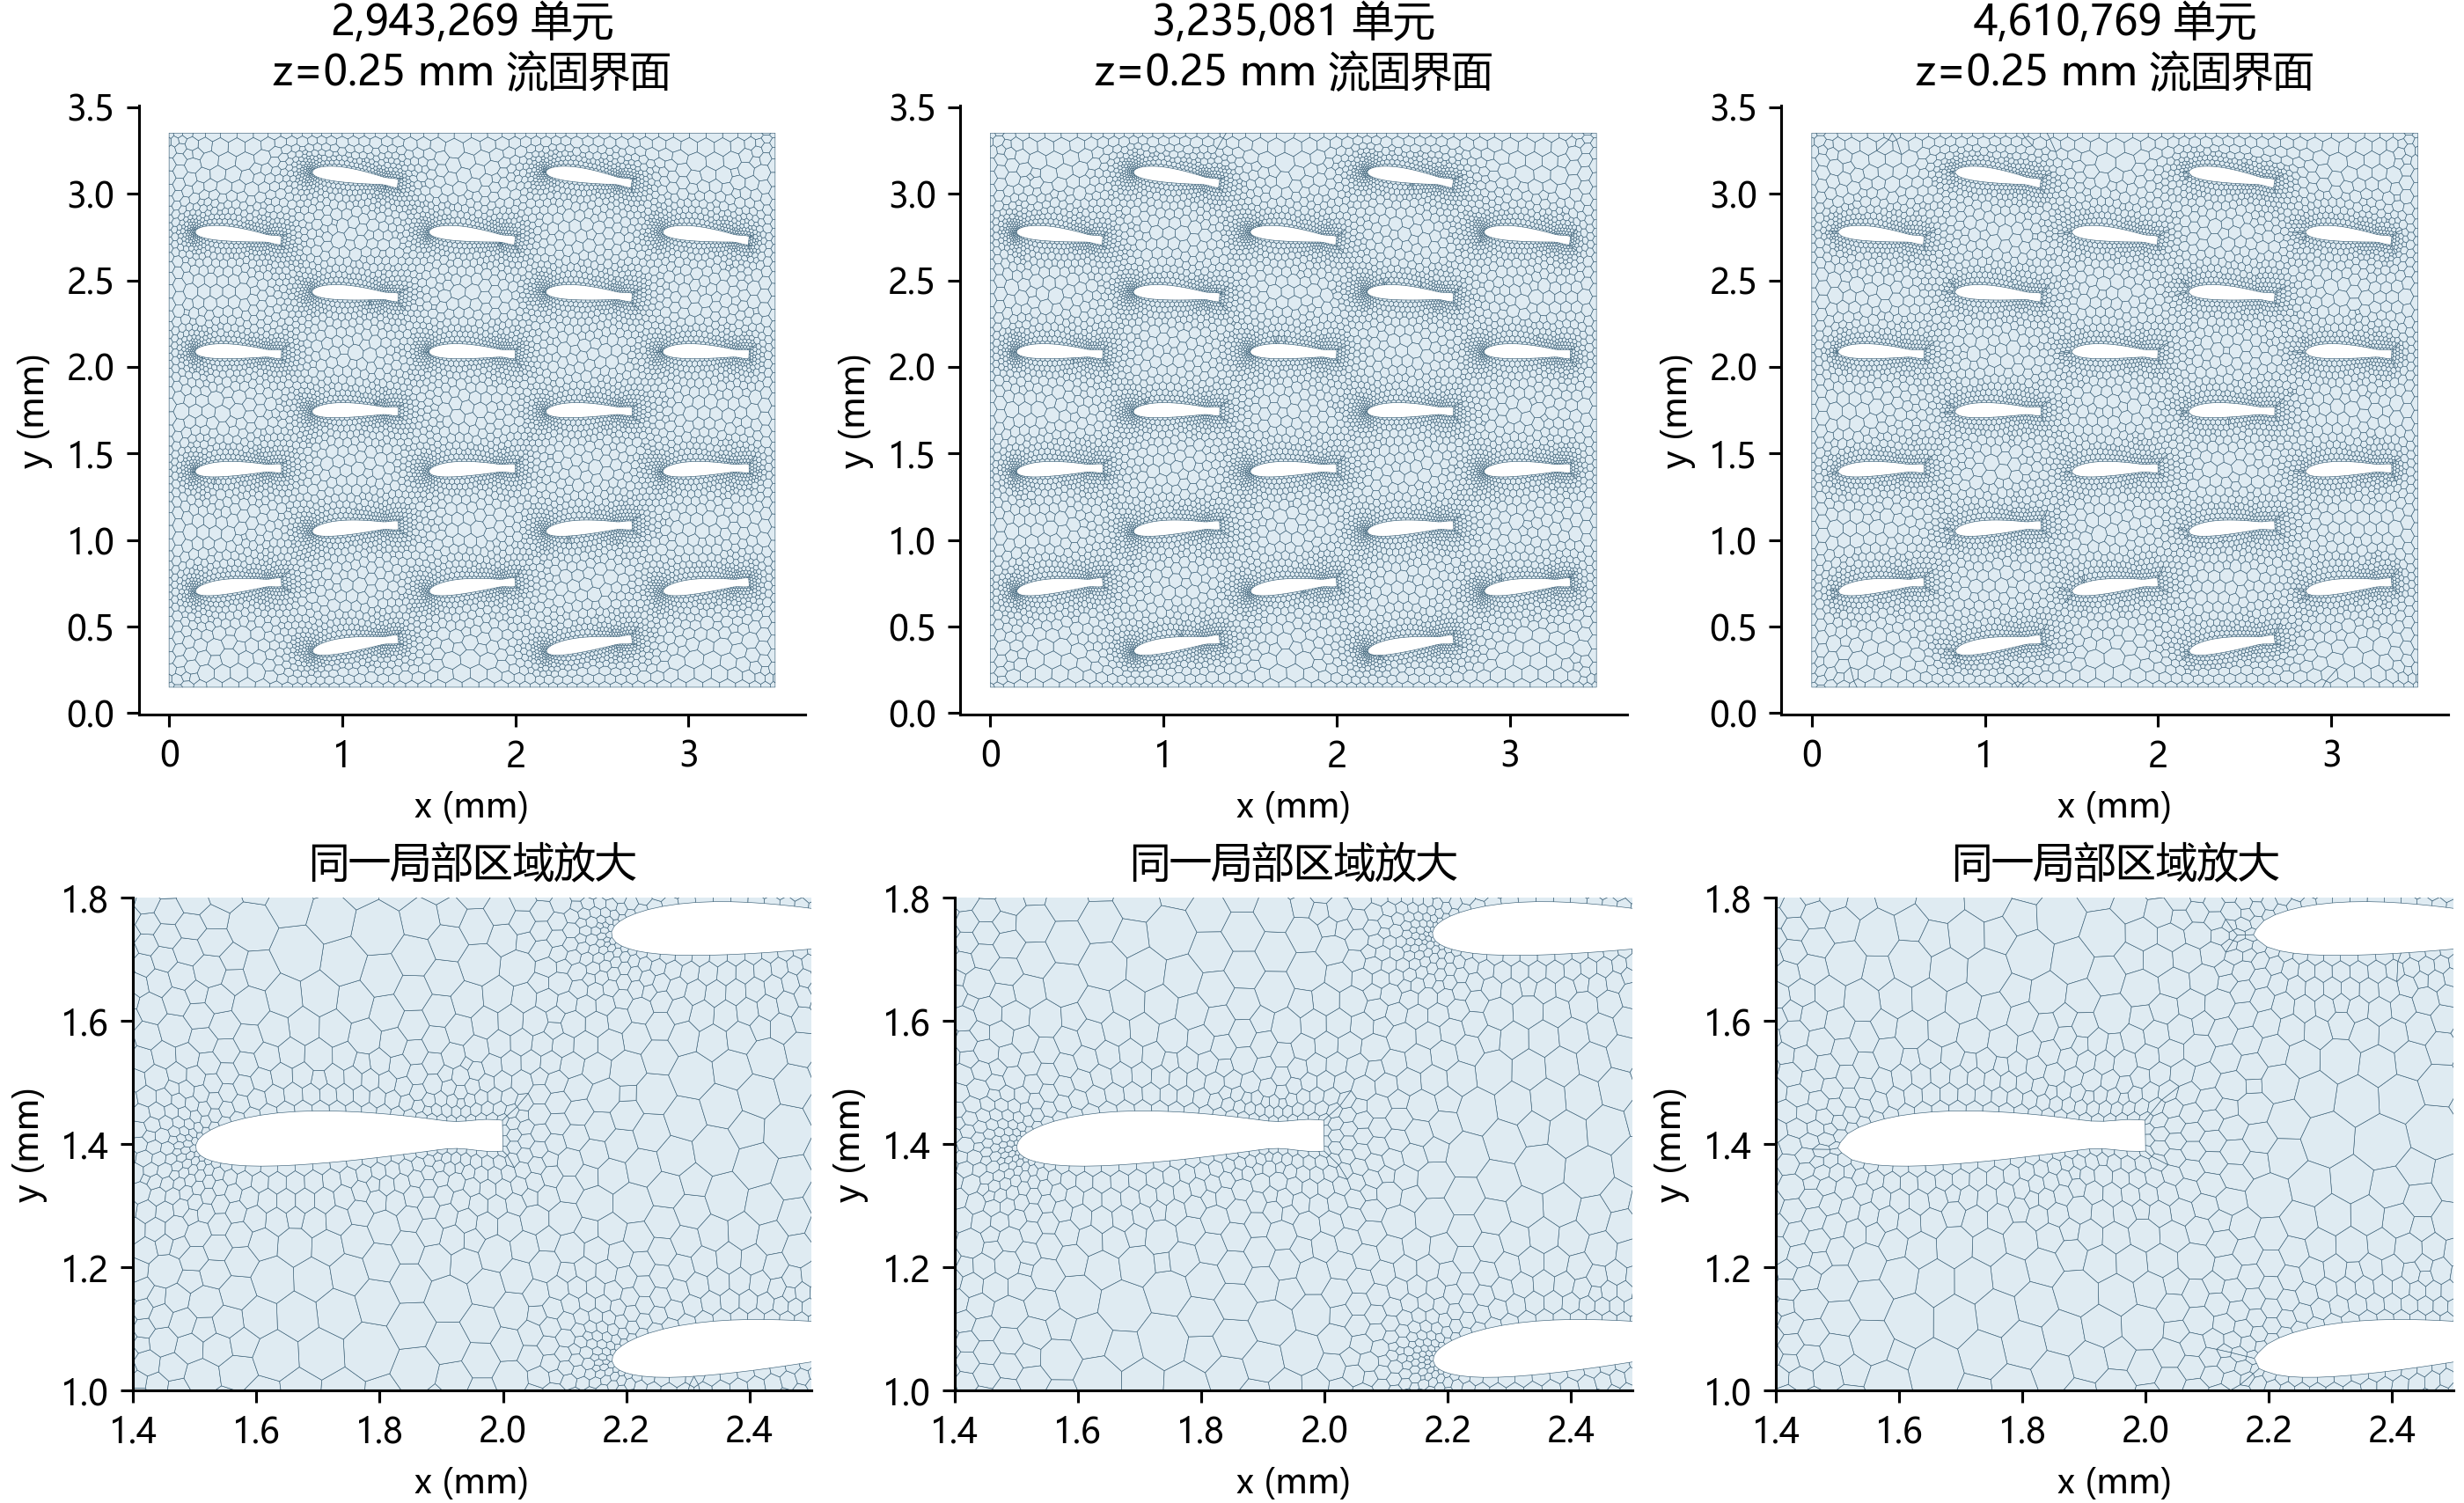
\includegraphics[width=\linewidth]{figs/midterm_asset_naca_mesh_actual.png}
\caption{NACA2416 v3三档实际流固界面面网格，统一取 z=0.25 mm。下排采用相同局部范围；此图不等同于三维边界层截面，单元总数增大也不保证每一局部区域同步加密。}\label{fig:08}
\end{subfigure}\hfill
\begin{subfigure}{0.49\linewidth}\centering
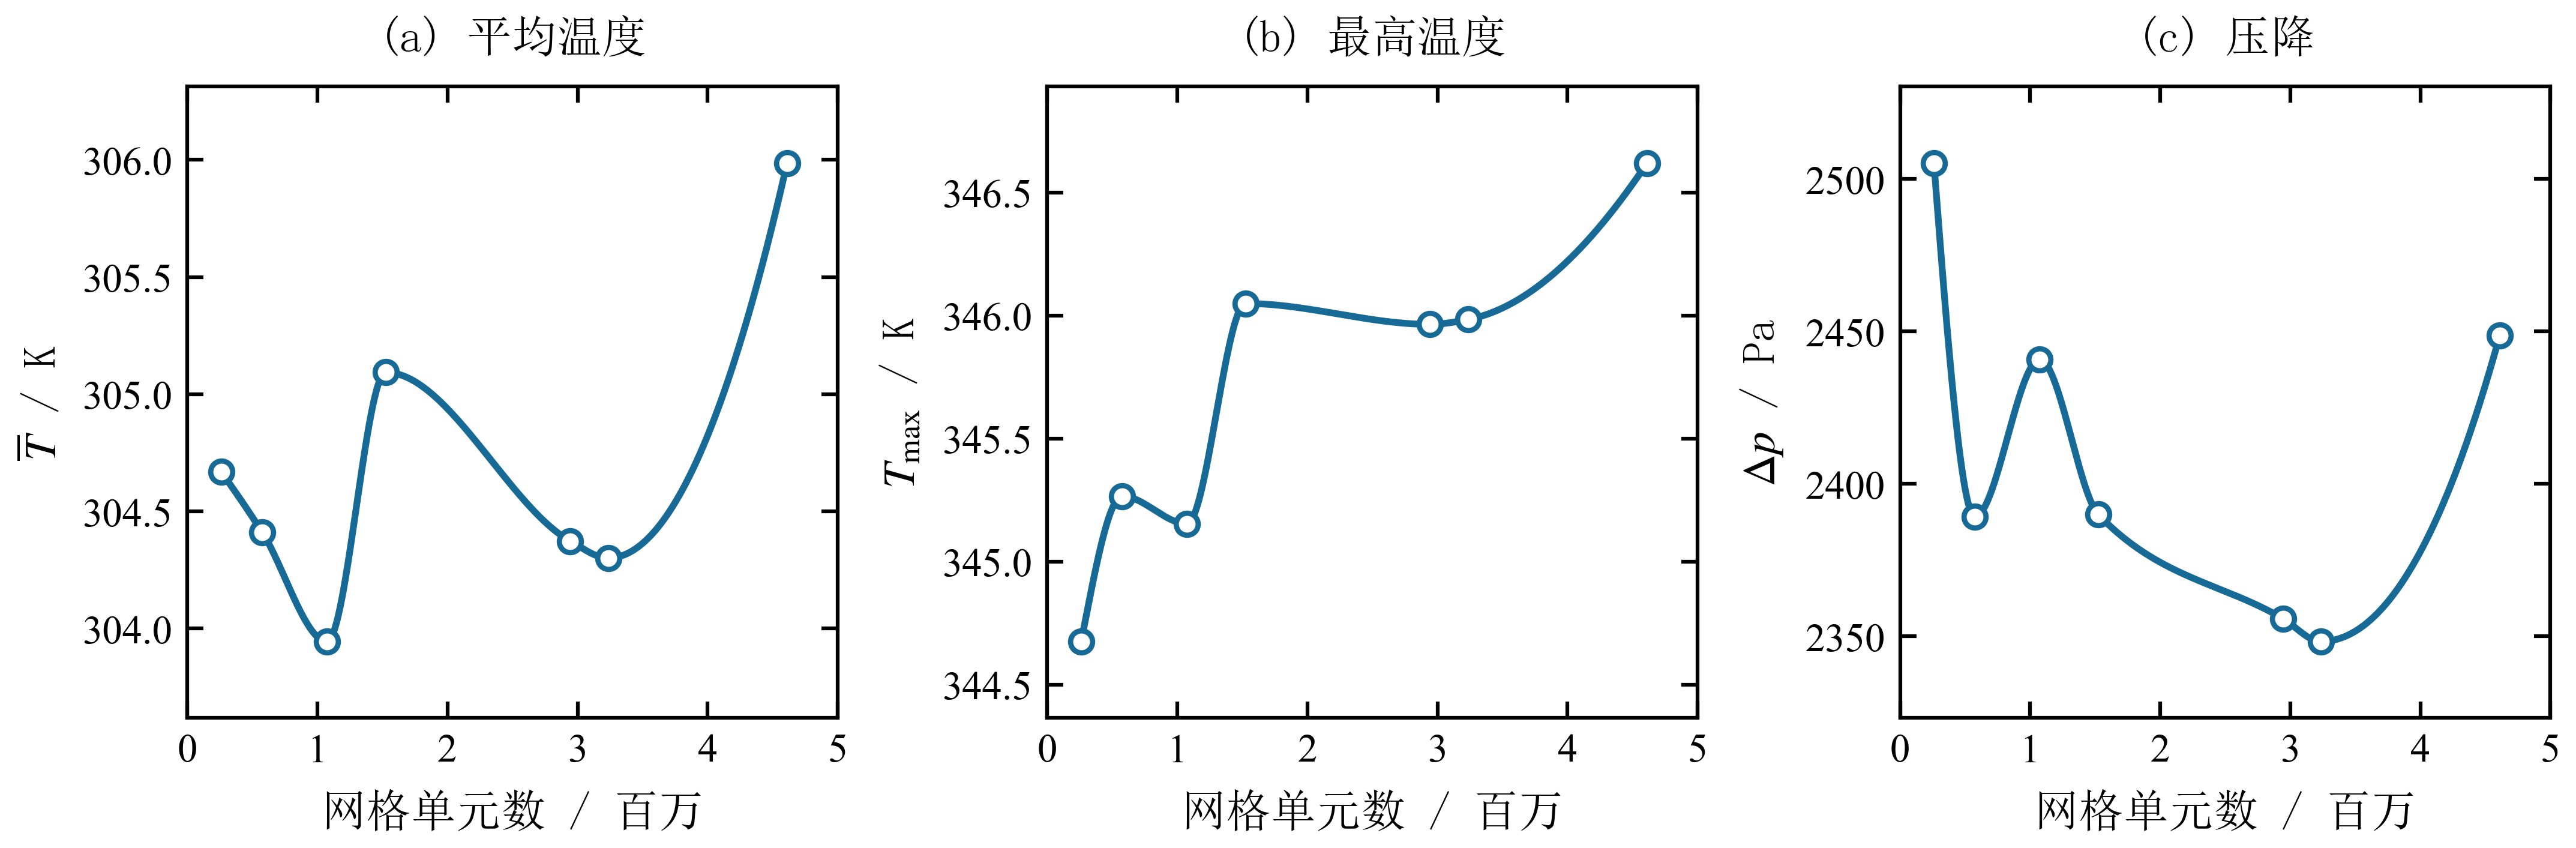
\includegraphics[width=\linewidth]{figs/midterm_month3_mesh_temperature_pressure.png}
\caption{NACA2416在0.2 s的七档网格温度与静压差，沿用原始保存数据。}\label{fig:09}
\end{subfigure}
\caption{流固界面面网格与七档网格温度、静压差}
\end{figure}



本阶段统一以 $N_{\mathrm{ref}}=3\,235\,081$ 为比较参考，按
$e_{\phi,i}=|\phi_i-\phi_{\mathrm{ref}}|/|\phi_{\mathrm{ref}}|\times100\%$ 计算差异；
参考档并非精确解，参考档自身差异为零也不能证明网格无关。
表~\ref{m3:tab:mesh_ref323}和图~\ref{fig:mesh-errors}均采用同一分母。
\begin{table}[!htbp]\centering
\caption{以323万档为参考的温度与压降相对差异（\%）}
\label{m3:tab:mesh_ref323}
\begin{tabular*}{\textwidth}{@{\extracolsep{\fill}}rrrr@{}}\toprule
\rowcolor{ydzjlight} 单元数 / 万 & 平均温度差异 & 最高温度差异 & 压降差异 \\
\midrule
26.02 & 0.1208 & 0.3782 & 6.6807 \\
57.51 & 0.0363 & 0.2076 & 1.7440 \\
107.36 & 0.1170 & 0.2400 & 3.9367 \\
152.49 & 0.2604 & 0.0188 & 1.7722 \\
294.33 & 0.0239 & 0.0057 & 0.3201 \\
323.51 & 0.0000 & 0.0000 & 0.0000 \\
461.08 & 0.5537 & 0.1835 & 4.2751 \\
\bottomrule\end{tabular*}\end{table}

294万档相对323万档的平均温度、最高温度和压降差异分别为0.0239\%、0.0057\%和0.3201\%，
对应绝对差约0.0726 K、0.0198 K和7.518 Pa；该局部区间较接近。
152万档压降差异仍为1.7722\%，461万档为4.2751\%，现有记录不支持“约150万网格已验证”的判断。当前323万档用于诊断与成本折中，尚未成为全部新构型的通用生产网格。
流体侧 $D_h=2.8070$ mm、$L=3.5$ mm时，323万档 $Nu=175.818$、
$h_c\approx38210.0$ W/(m$^2$·K)；294万档二者差异约0.11\%，461万档约1.54\%，
$f_D$差异约4.28\%。$Re\approx6603$只用于记录该特征尺度下的流动量级，
并不单独证明层流模型在全部参数范围有效，后续还需结合扰流结构和流动形态复核。

\begin{figure}[!htbp]\centering
\begin{subfigure}{0.49\linewidth}\centering
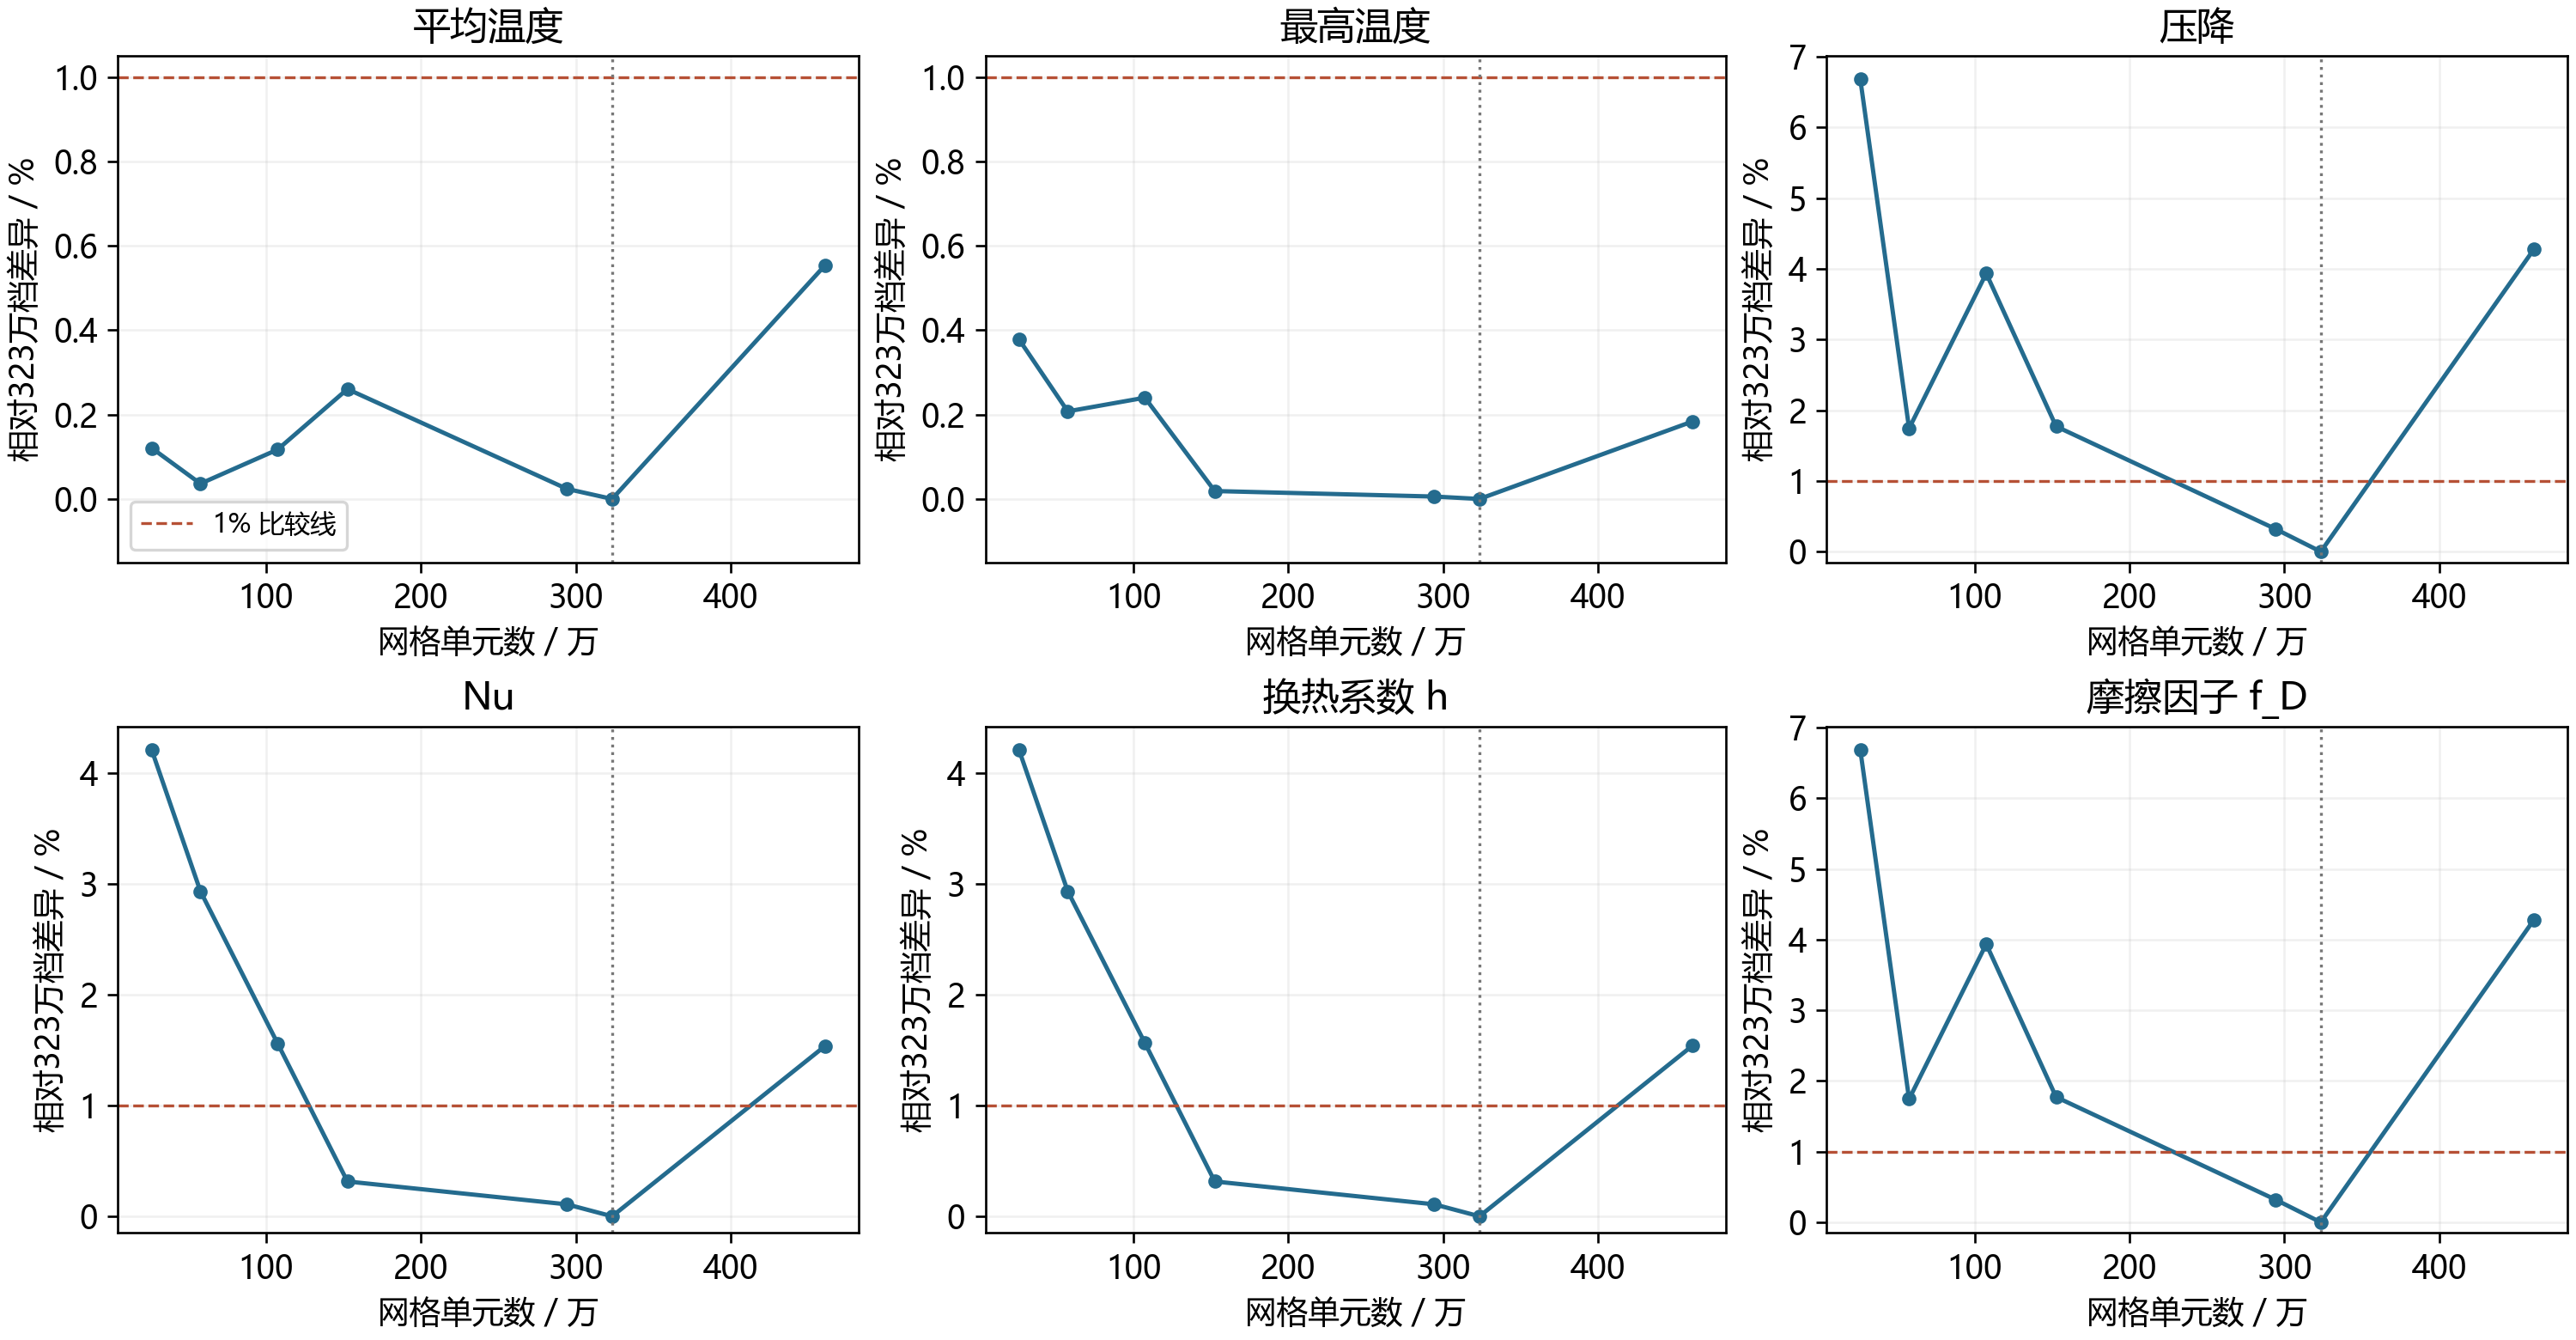
\includegraphics[width=\linewidth]{figs/midterm_month3_mesh_errors_ref323.png}
\caption{温度、压降及换热流阻指标统一以323万档为参考的相对差异，虚线为1\%比较线。}\label{fig:mesh-errors}
\end{subfigure}\hfill
\begin{subfigure}{0.49\linewidth}\centering
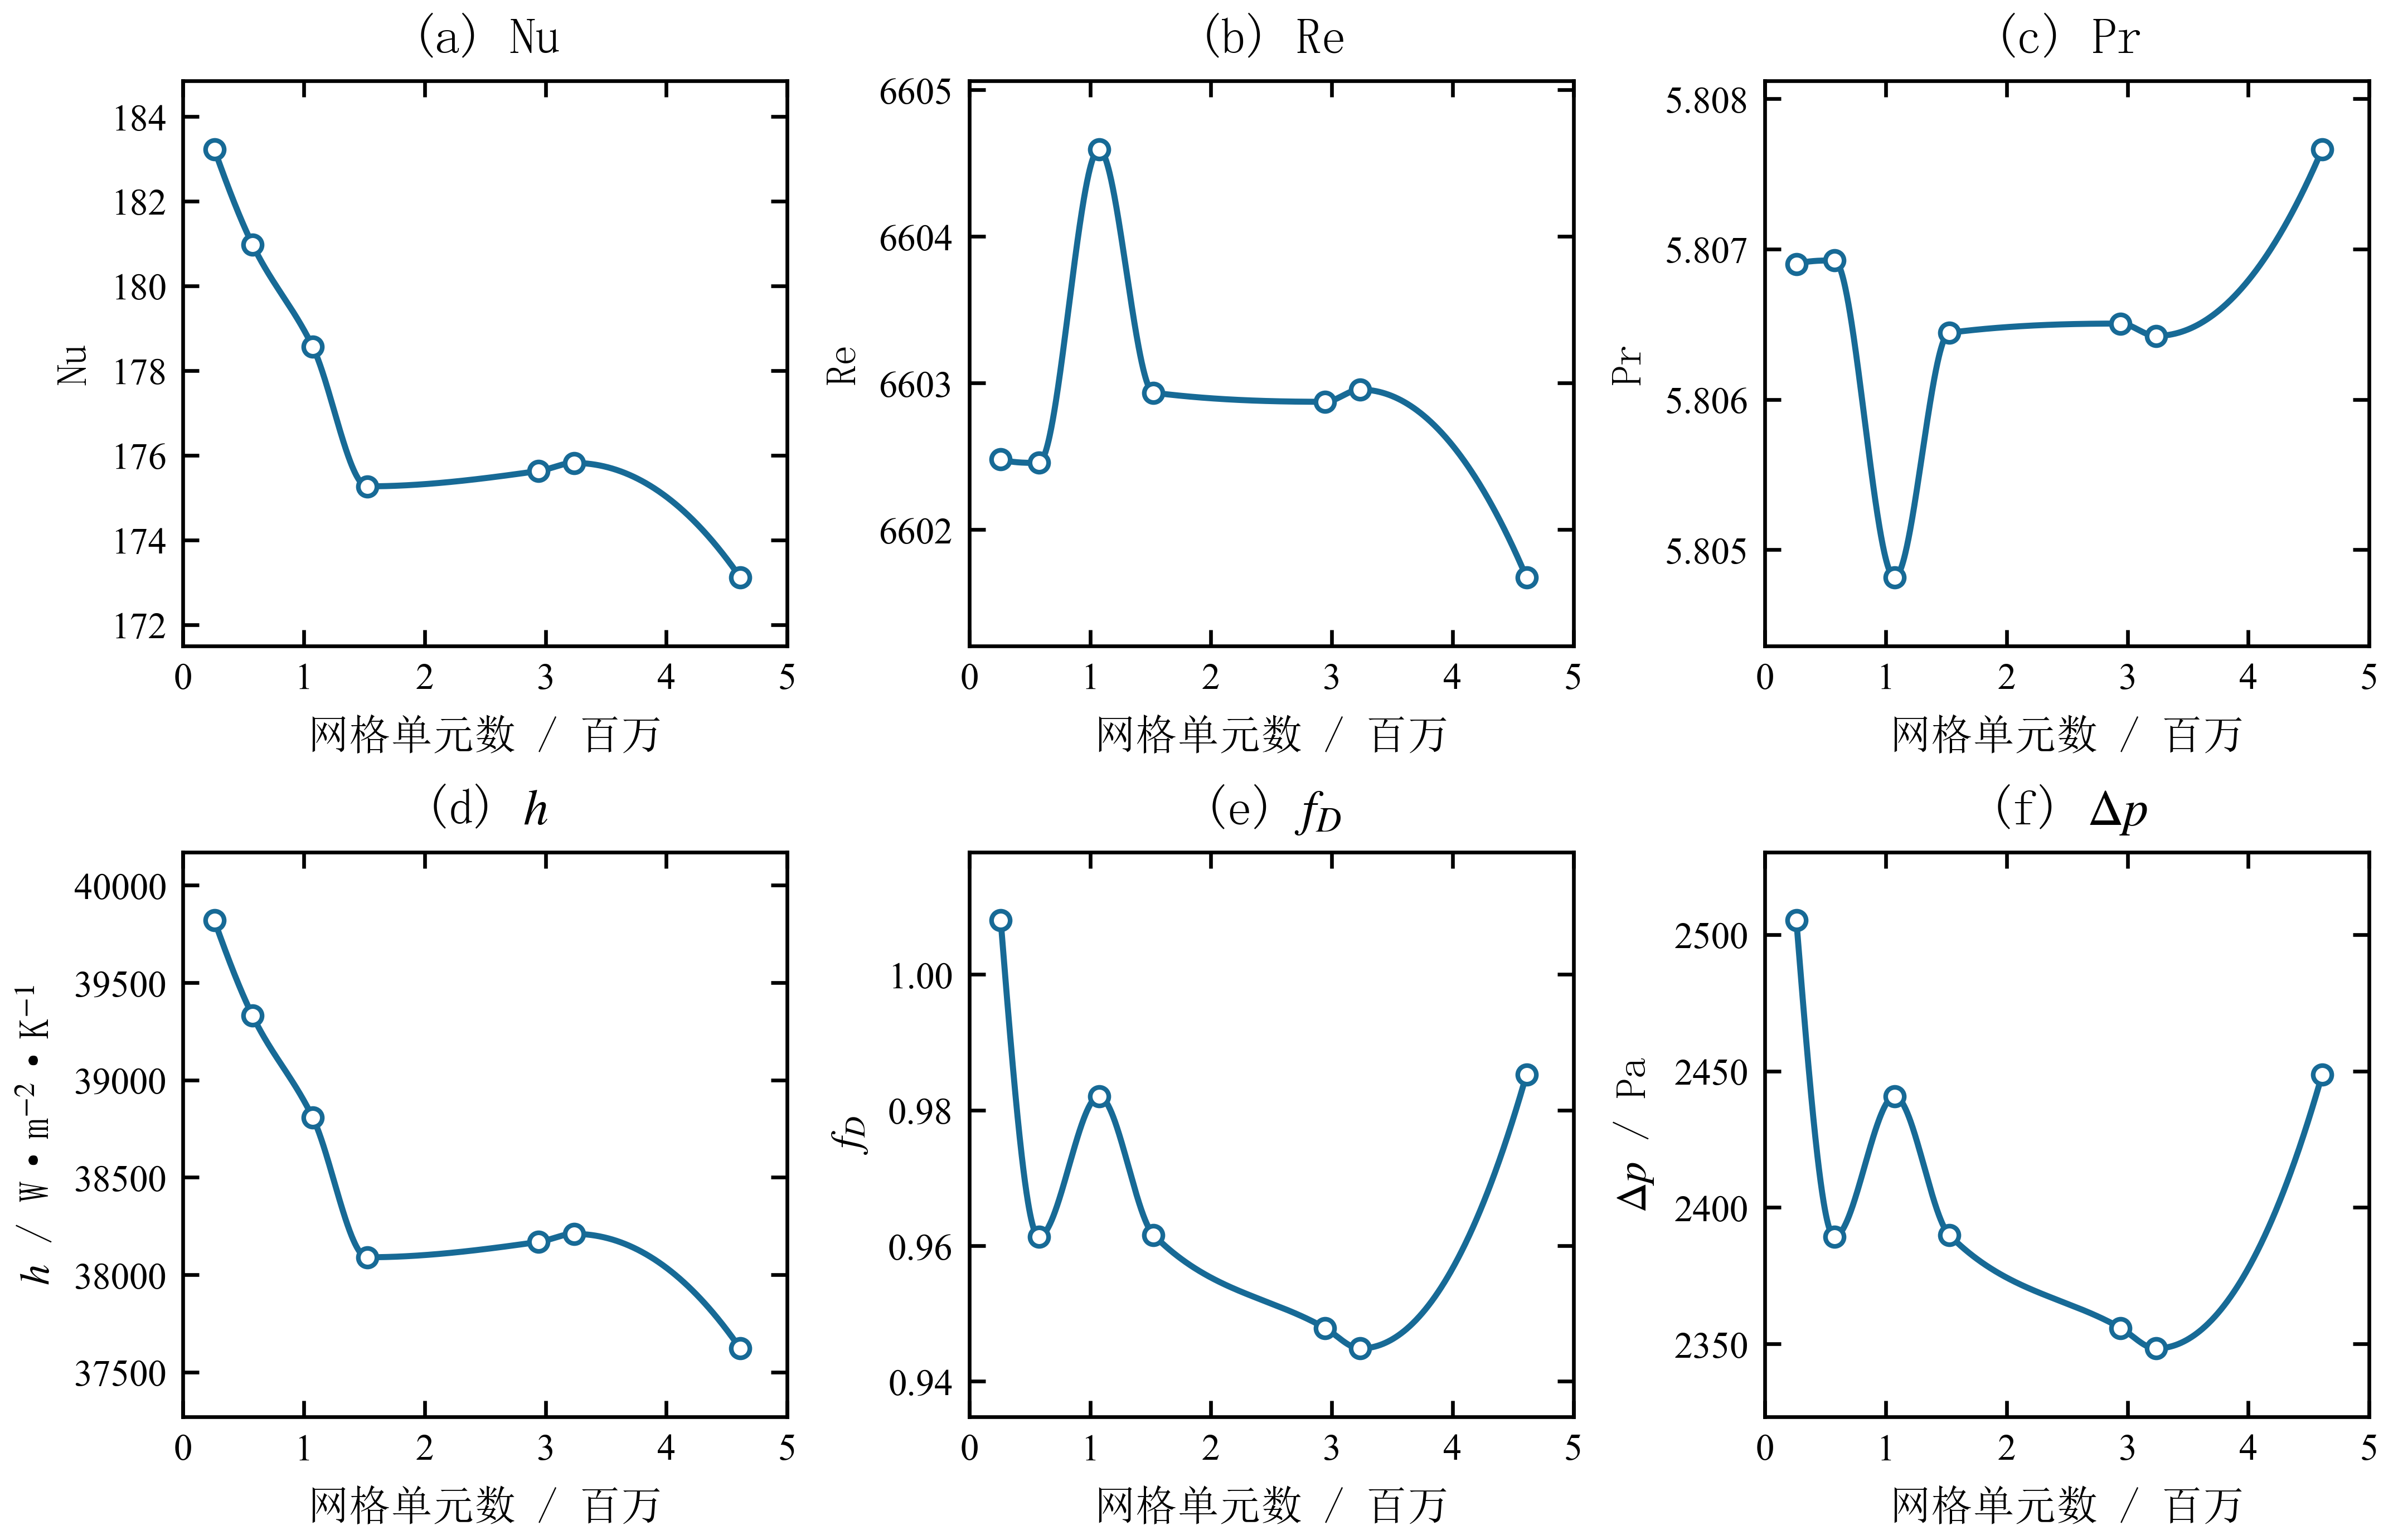
\includegraphics[width=\linewidth]{figs/midterm_month3_mesh_dimensionless.png}
\caption{七档网格的换热与流阻指标；特征尺度、物性参考温度及热流统计沿用原始保存记录。}\label{fig:mesh-dimensionless}
\end{subfigure}
\caption{以323万档为参考的相对差异与无量纲换热流阻指标}
\end{figure}

图~\ref{fig:mesh-dimensionless}给出七档网格的换热与流阻指标。
图~\ref{fig:mesh-flow}与图~\ref{fig:mesh-outlet}按相同色标比较323万与461万档。
前者显示 $z=1.50$ mm平面的主流向速度、投影流线、温度与静压；投影流线并非完整三维轨迹。
后者显示出口法向速度和温度。两档出口回流面积比例分别为5.1720\%和5.3886\%，
回流质量流量占入口流量分别为0.4754\%和0.2777\%；回流面积扩大而回流质量减少，
不能概括为461万档的回流整体更严重。两档回流面质量加权温度均为305 K。

\begin{figure}[!htbp]\centering
\begin{subfigure}{0.49\linewidth}\centering
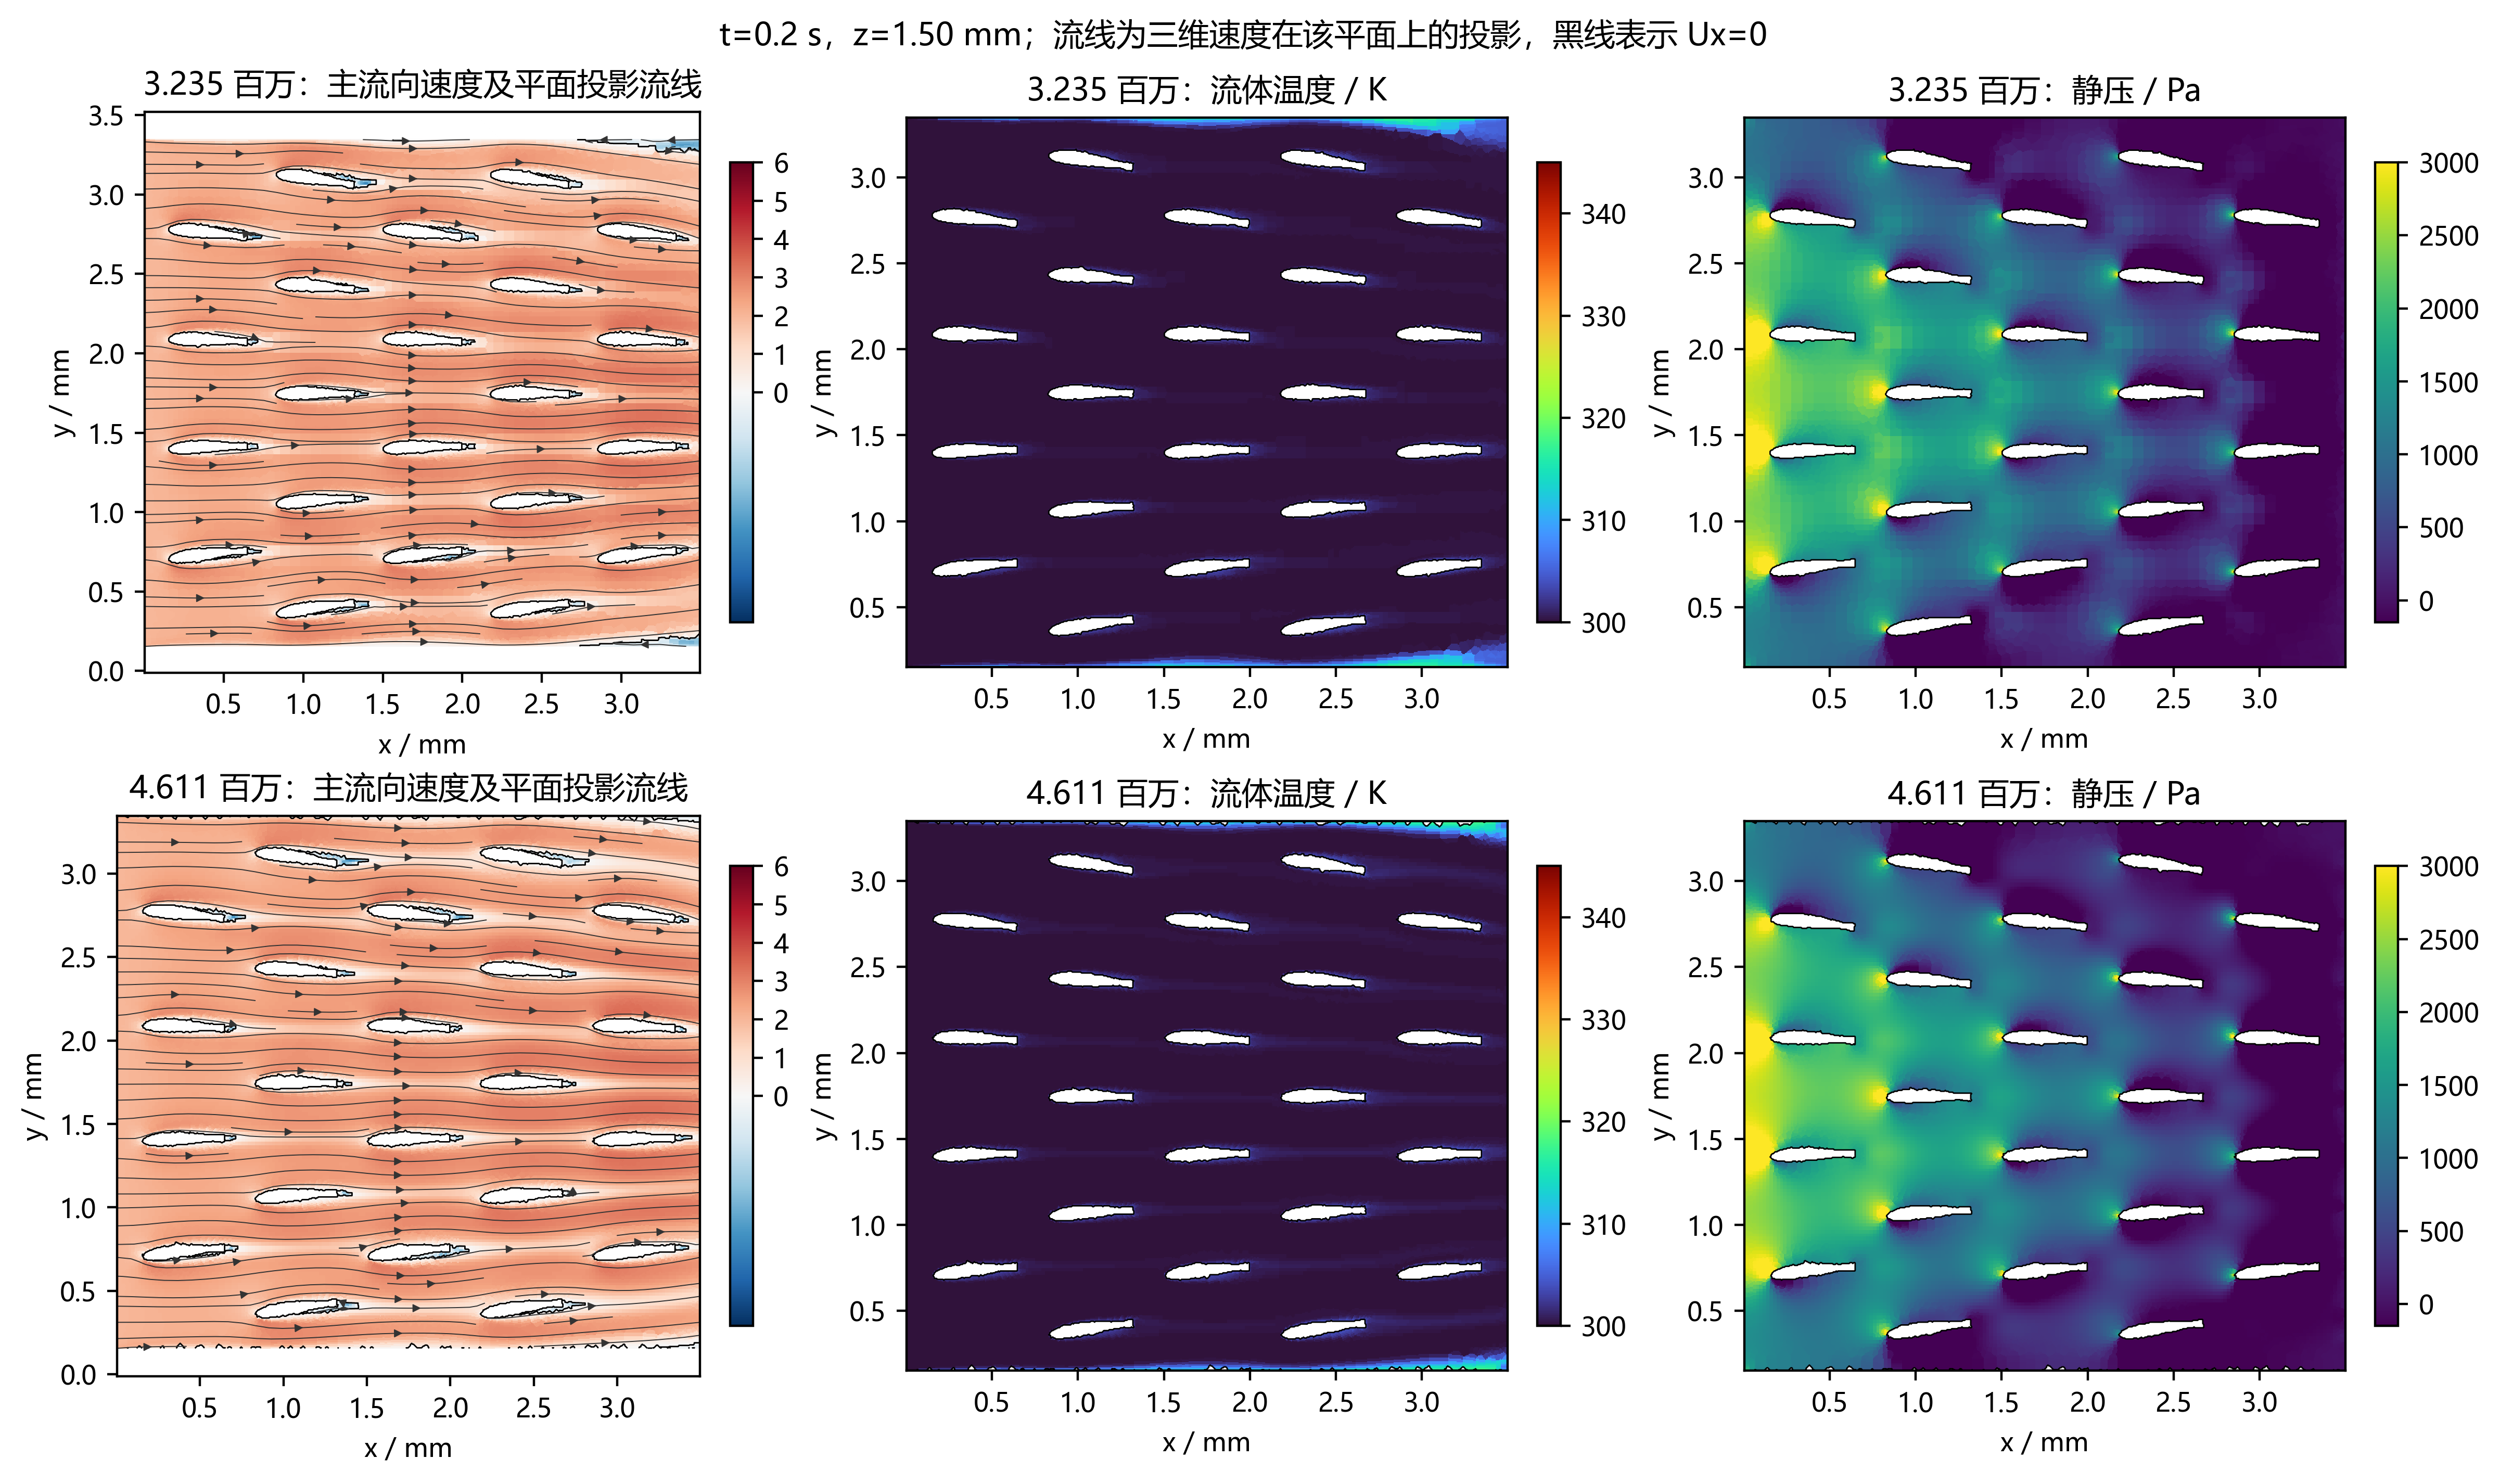
\includegraphics[width=\linewidth]{figs/midterm_month3_mesh_flowfield.png}
\caption{323万档（上排）与461万档（下排）的中高平面速度、投影流线、温度和静压。}\label{fig:mesh-flow}
\end{subfigure}\hfill
\begin{subfigure}{0.49\linewidth}\centering
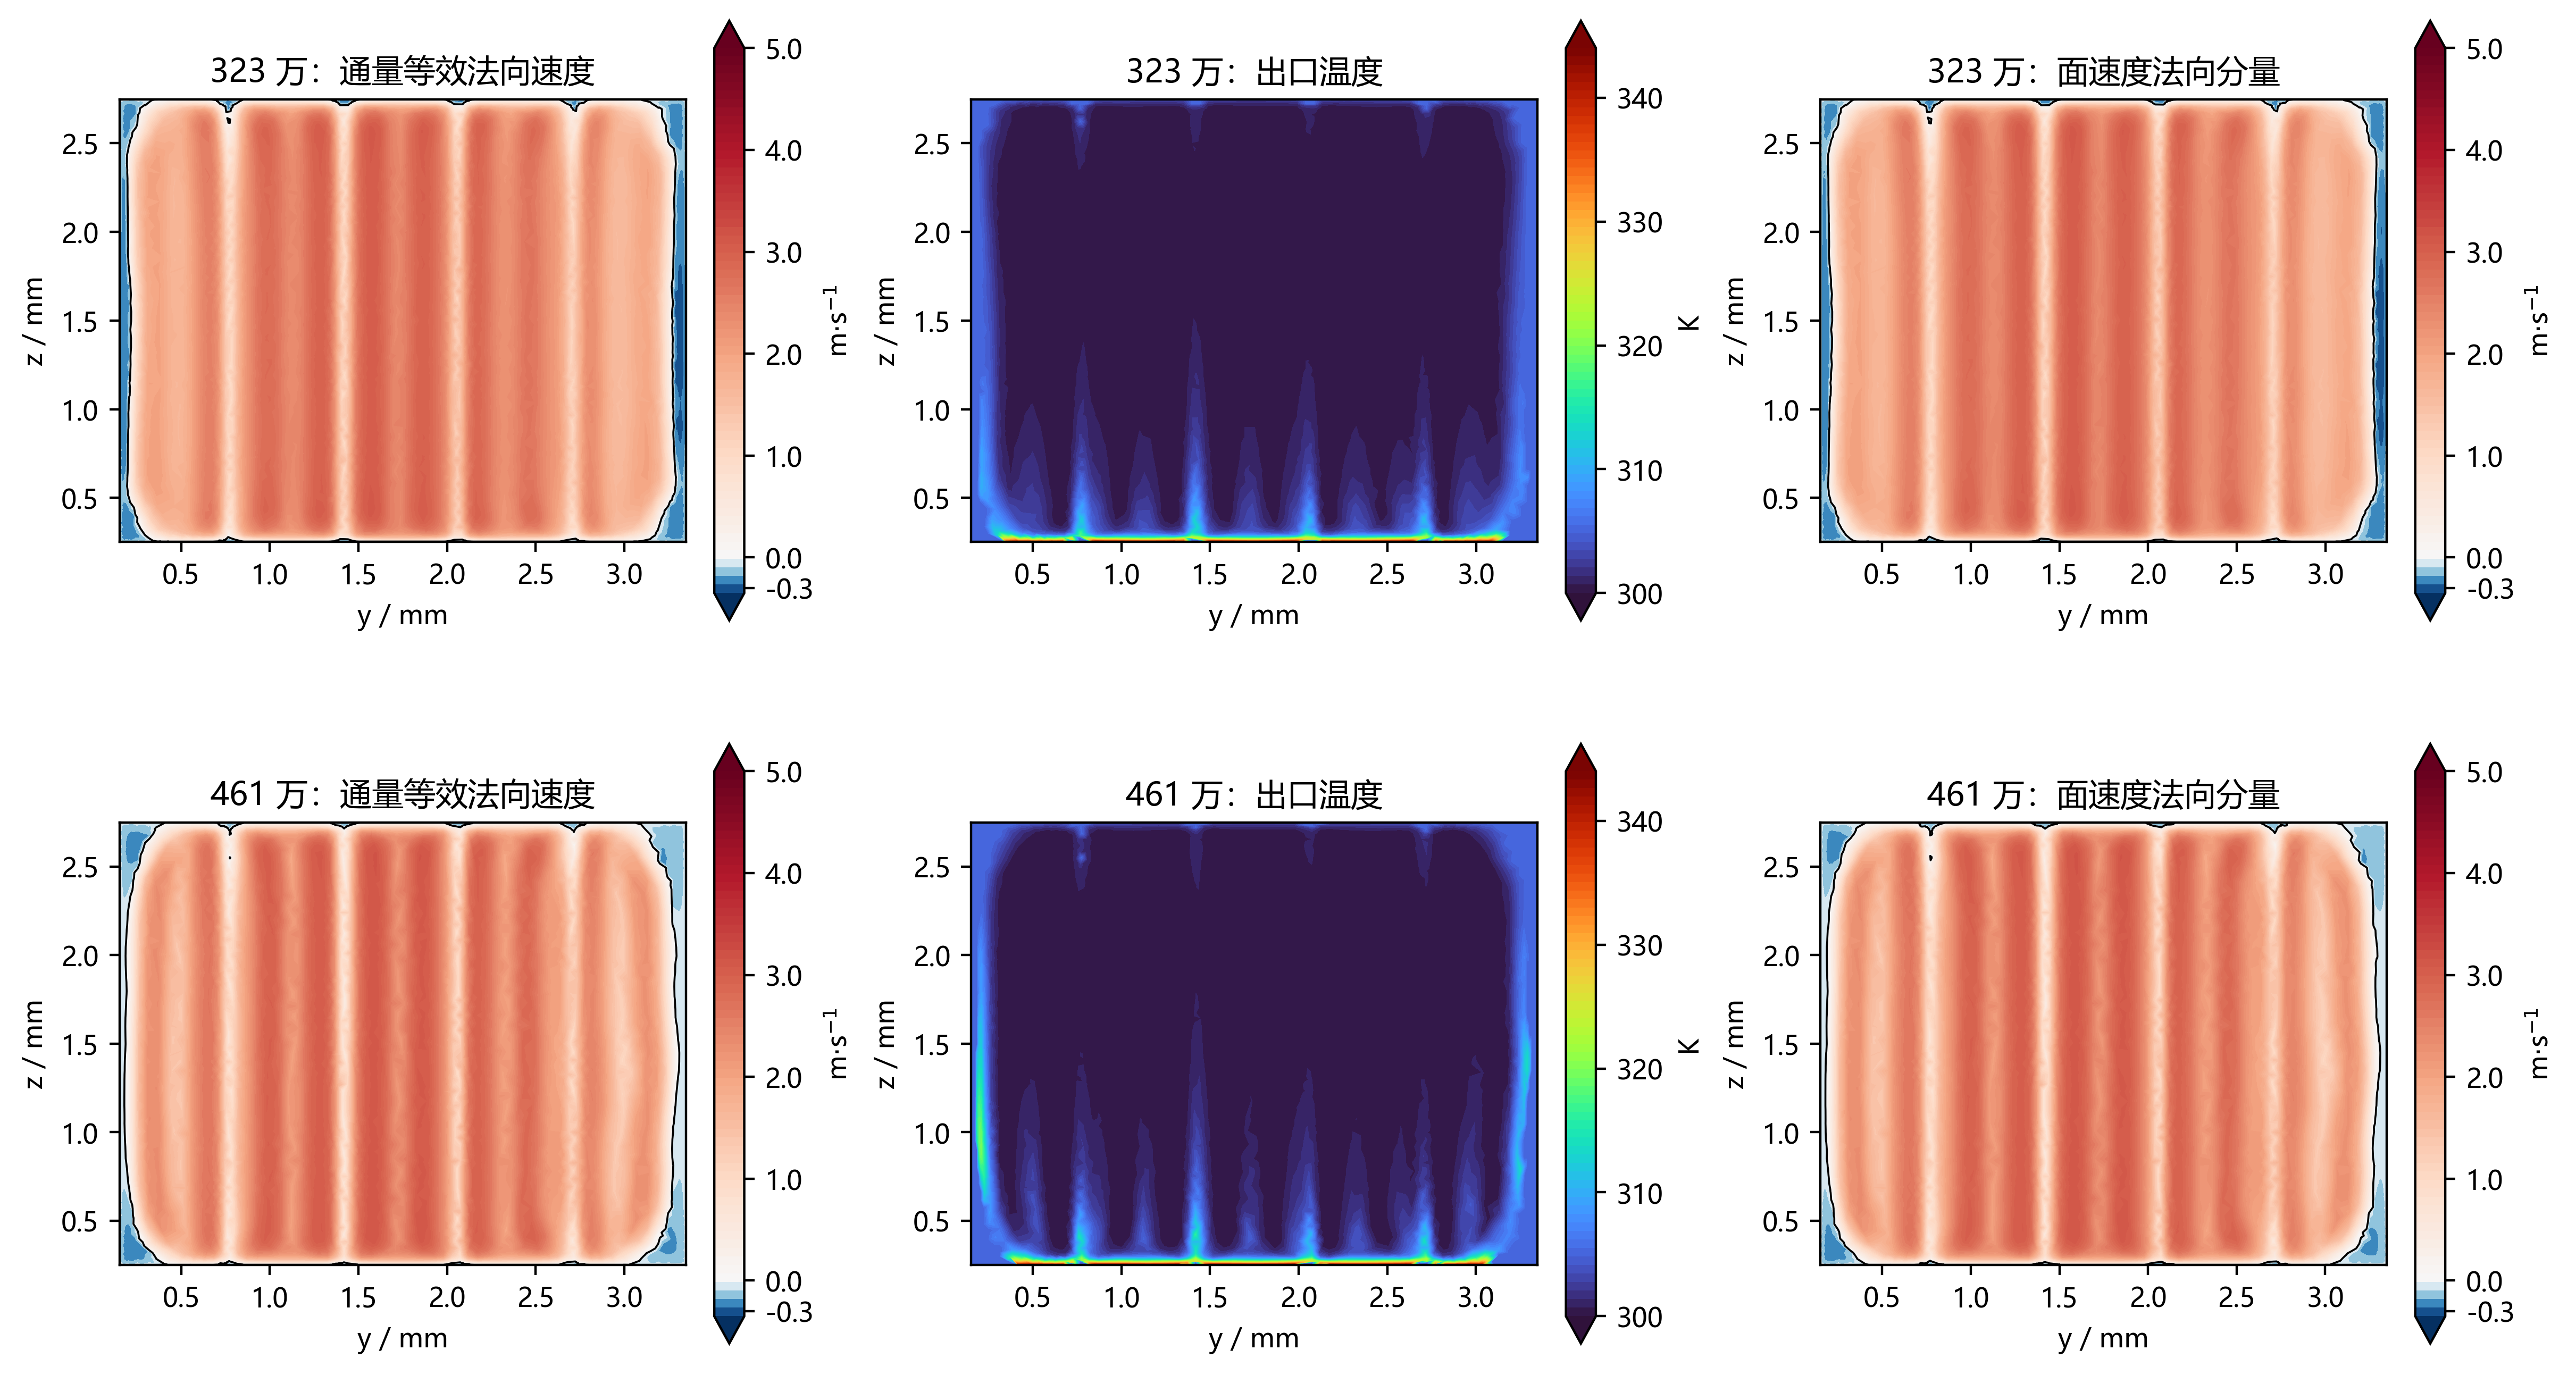
\includegraphics[width=\linewidth]{figs/midterm_month3_mesh_outlet.png}
\caption{323万档（上排）与461万档（下排）的出口速度和温度。出口局部回流与内部尾迹分开识别。}\label{fig:mesh-outlet}
\end{subfigure}
\caption{两种网格档的中高平面流场与出口截面}
\end{figure}

同区域体积加权温度为305.7793 K与305.8673 K，相对323万档差约0.0288\%，
远小于单元算术平均的0.5537\%；这说明平均方式和网格统计权重会显著影响结论。
尚未进行统一时间推进历史、出口延长或回流温度敏感性重算，因此不能将压降差异直接归因于单一出口因素。
GCI外推与两档相对差异也需区分：以323万为细档的107万／152万／323万组合压降形式GCI为0.7275\%，
表观阶约5.57；这不证明所有输出均已进入可信渐近区间\cite{stagereports}。
\subsubsection{物性实现对照}
补充资料在280--360 K、101325 Pa下核对1601个温度点。
密度、动力黏度、导热系数和比热的最大相对拟合误差分别为
0.0000151\%、0.0005164\%、0.0001216\%和0.0002054\%。
图~\ref{fig:udf-curves}保留原公式、REFPROP参考与最终拟合曲线；
图~\ref{fig:udf-fit-error}给出逐项最大误差。这是对同一参考物性的拟合检验，不等于物理模型的实验精度。
历史稿所述298.15 K密度偏低60.8\%与现有逐点公式核查表不一致：
该表中原公式密度为999.999985 kg/m$^3$，参考为997.047637 kg/m$^3$，偏高约0.2961\%。
现阶段保留来源差异，不继续沿用60.8\%作为当前已核实误差；后续需核对历史源码版本。

\begin{figure}[!htbp]\centering
\begin{subfigure}{0.49\linewidth}\centering
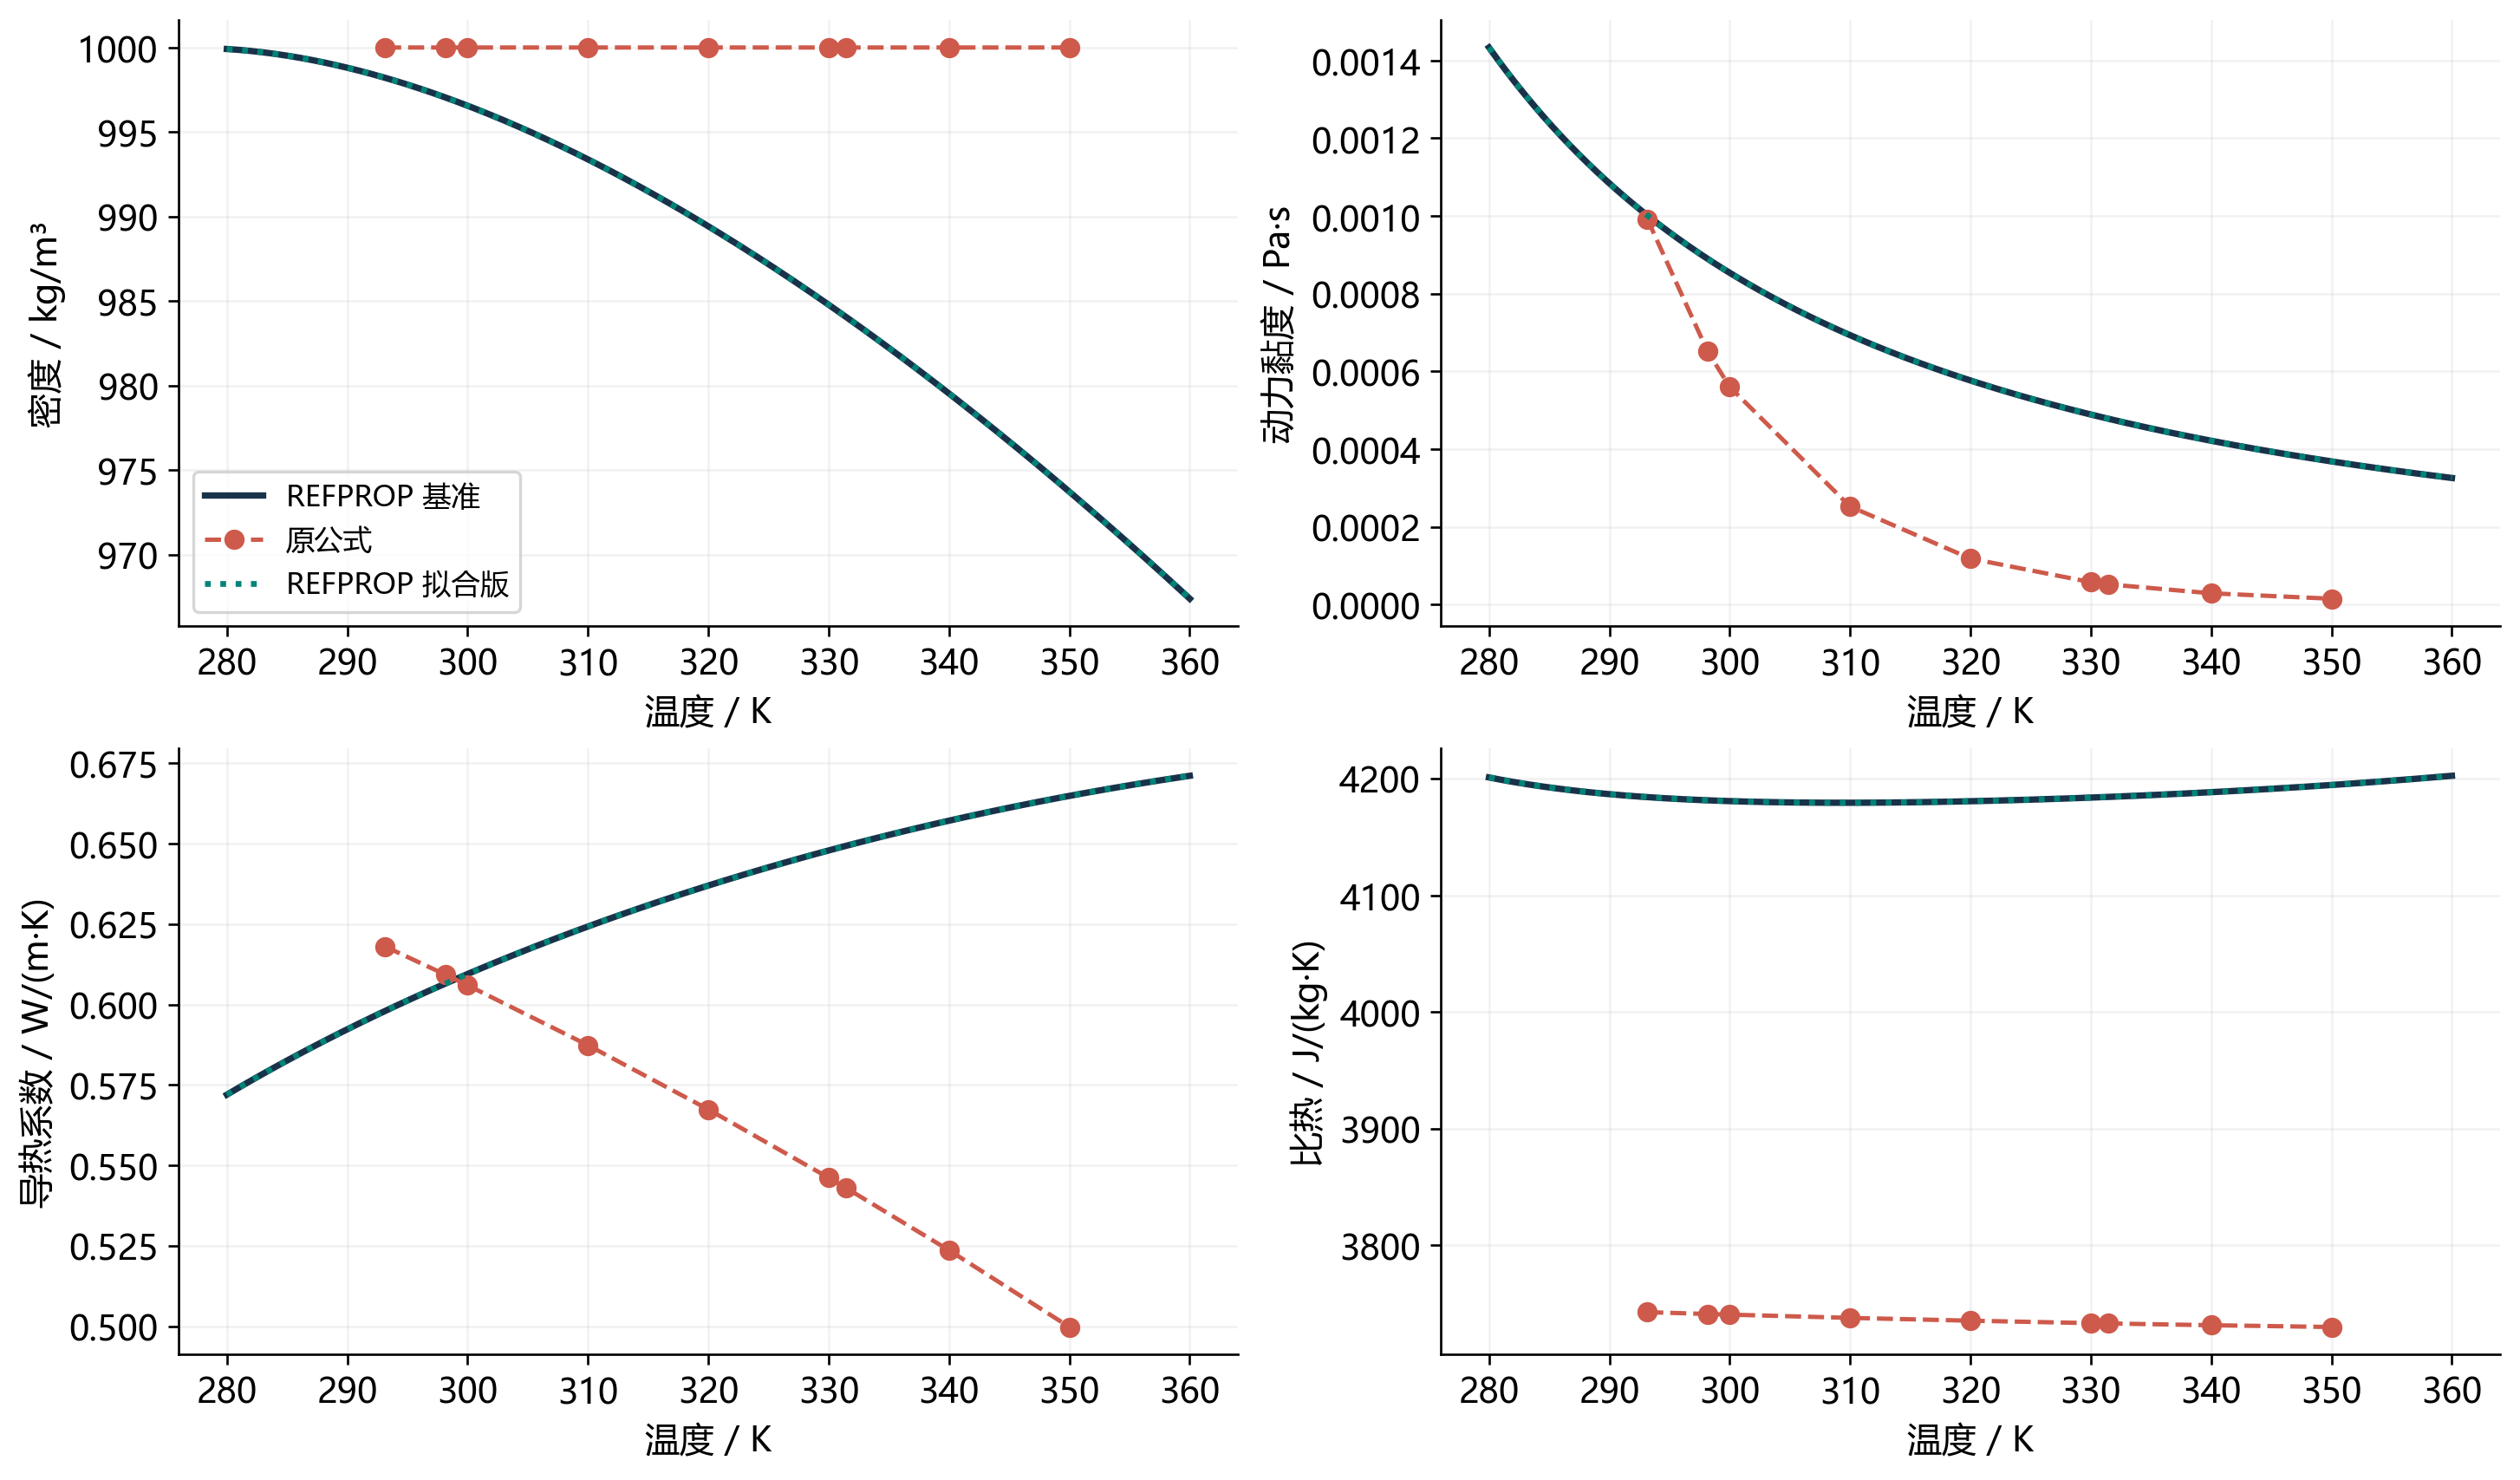
\includegraphics[width=\linewidth]{figs/midterm_asset_udf_01_四项物性温度曲线.png}
\caption{四项水物性随温度的变化：参考、原公式与最终REFPROP拟合版。排查候选公式与最终拟合版分别保留，不混用。}\label{fig:udf-curves}
\end{subfigure}\hfill
\begin{subfigure}{0.49\linewidth}\centering
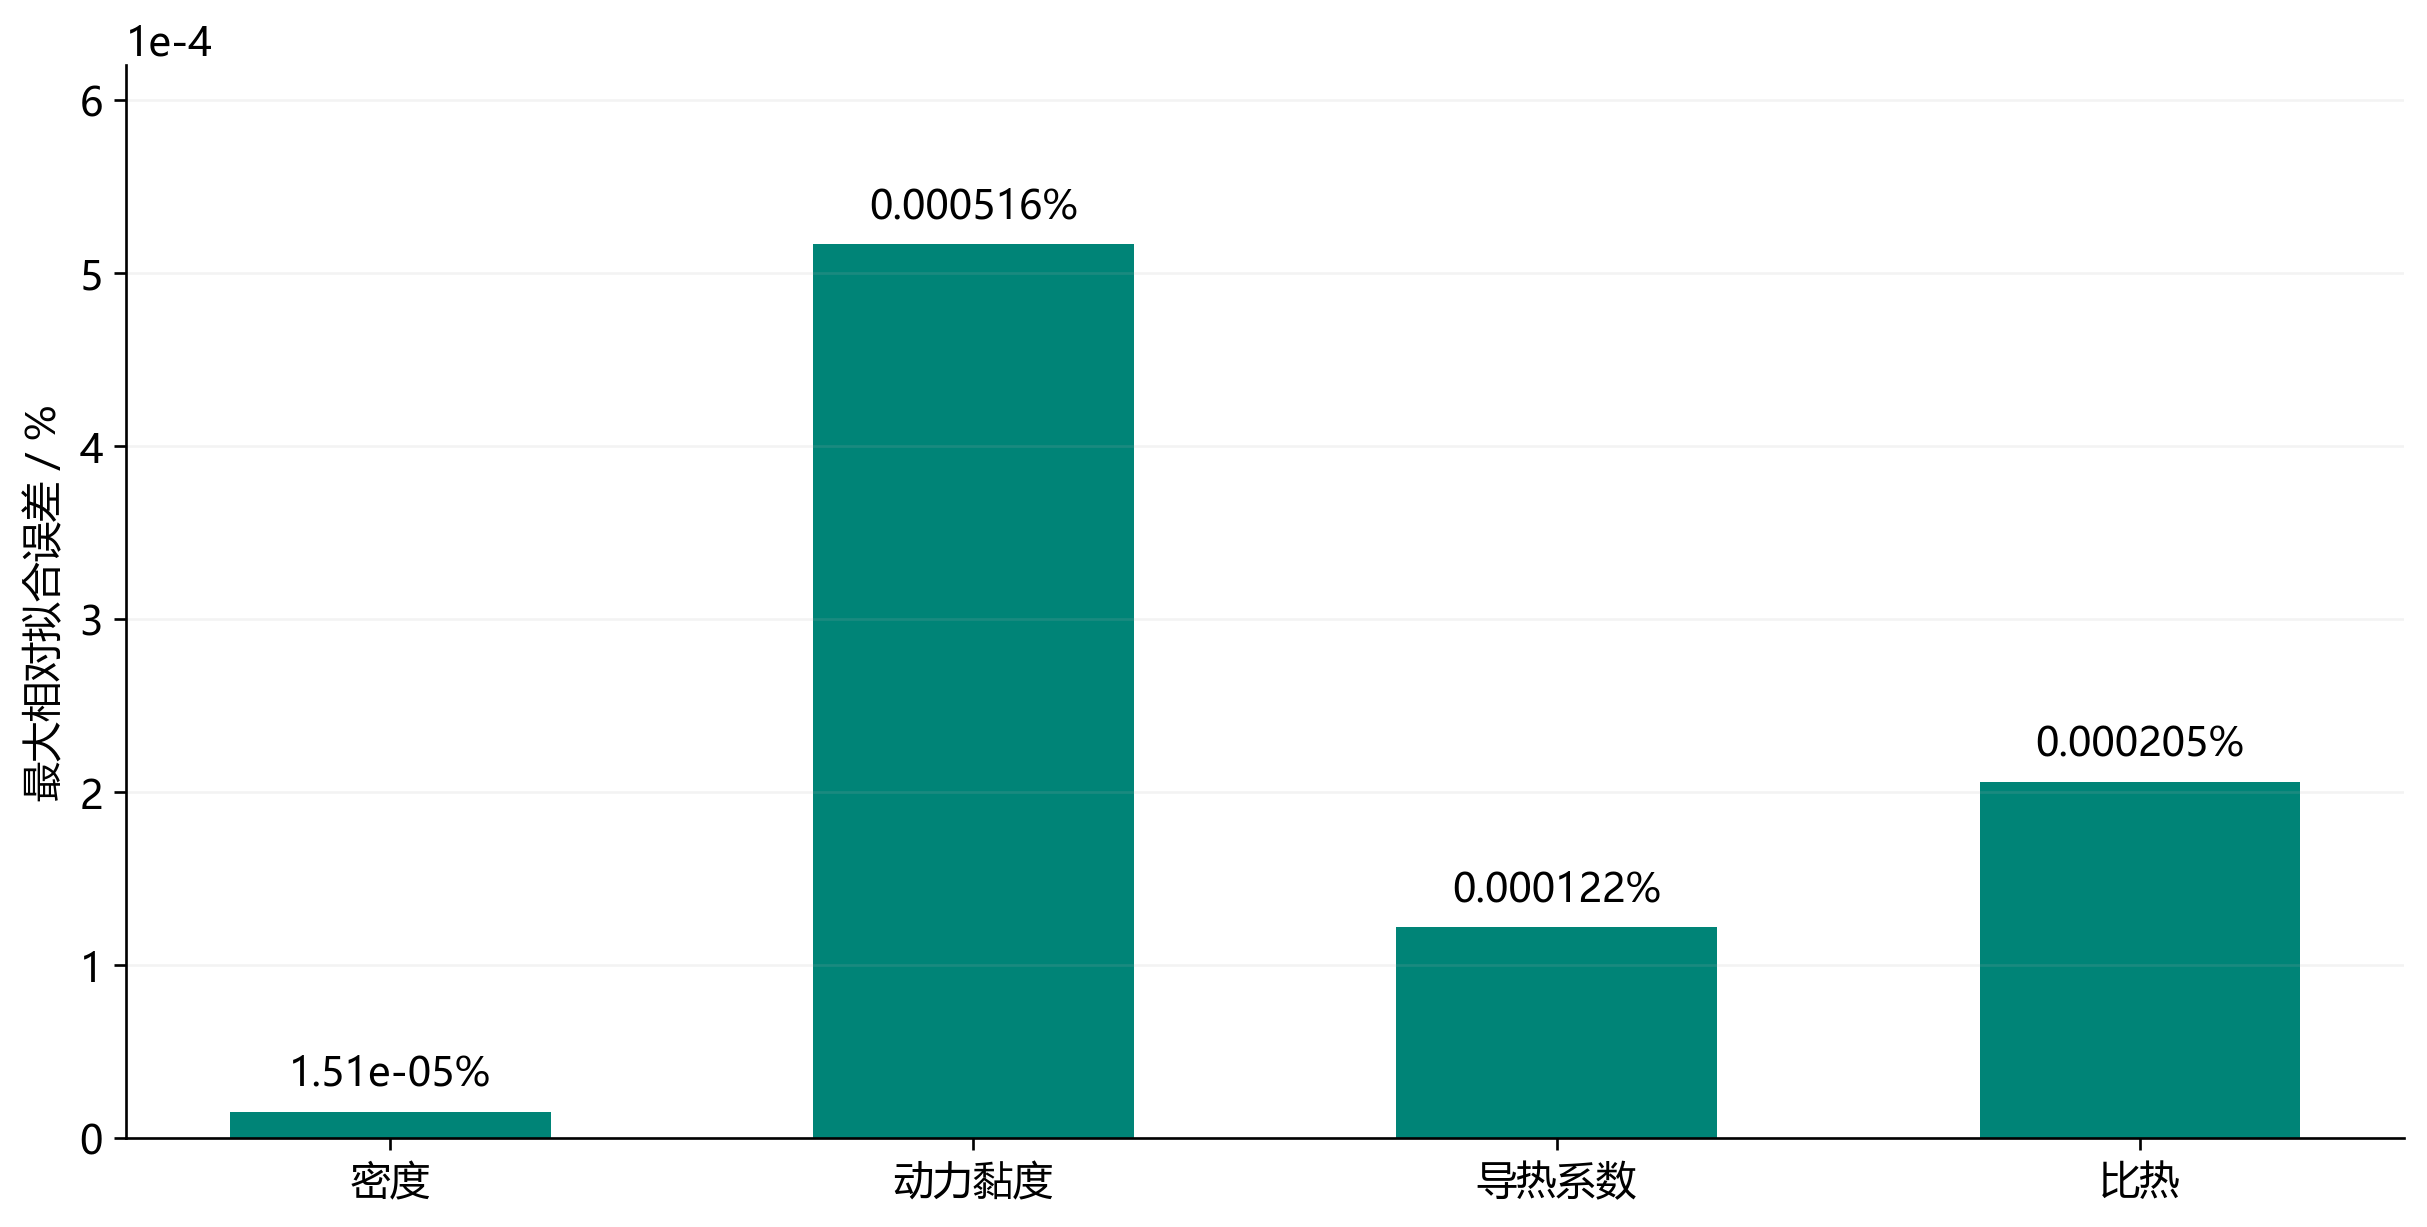
\includegraphics[width=\linewidth]{figs/midterm_asset_udf_03_1601点拟合误差.png}
\caption{1601温度点核对记录中的四项最大相对拟合误差。}\label{fig:udf-fit-error}
\end{subfigure}
\caption{物性随温度变化与1601点拟合误差}
\end{figure}

在共同0.137 s时刻，拟合与实时REFPROP实现的固体最高温度分别为332.6852693 K和332.6852725 K，
加热面最高温度分别为332.8039186 K和332.8039218 K；
进出口面积平均静压差分别为4290.169554 Pa和4290.159872 Pa。
共同前37步的求解及残差读取耗时分别为5.653 min和64.986 min，实时接口约为拟合版的11.50倍。
拟合分支最终到0.2 s，实时分支到0.137 s，因此末态文件不能直接逐点对比。
图~\ref{fig:udf-common}和图~\ref{fig:udf-time}分别保留共同时间段和共同步数口径。

\begin{figure}[!htbp]\centering
\begin{subfigure}{0.49\linewidth}\centering
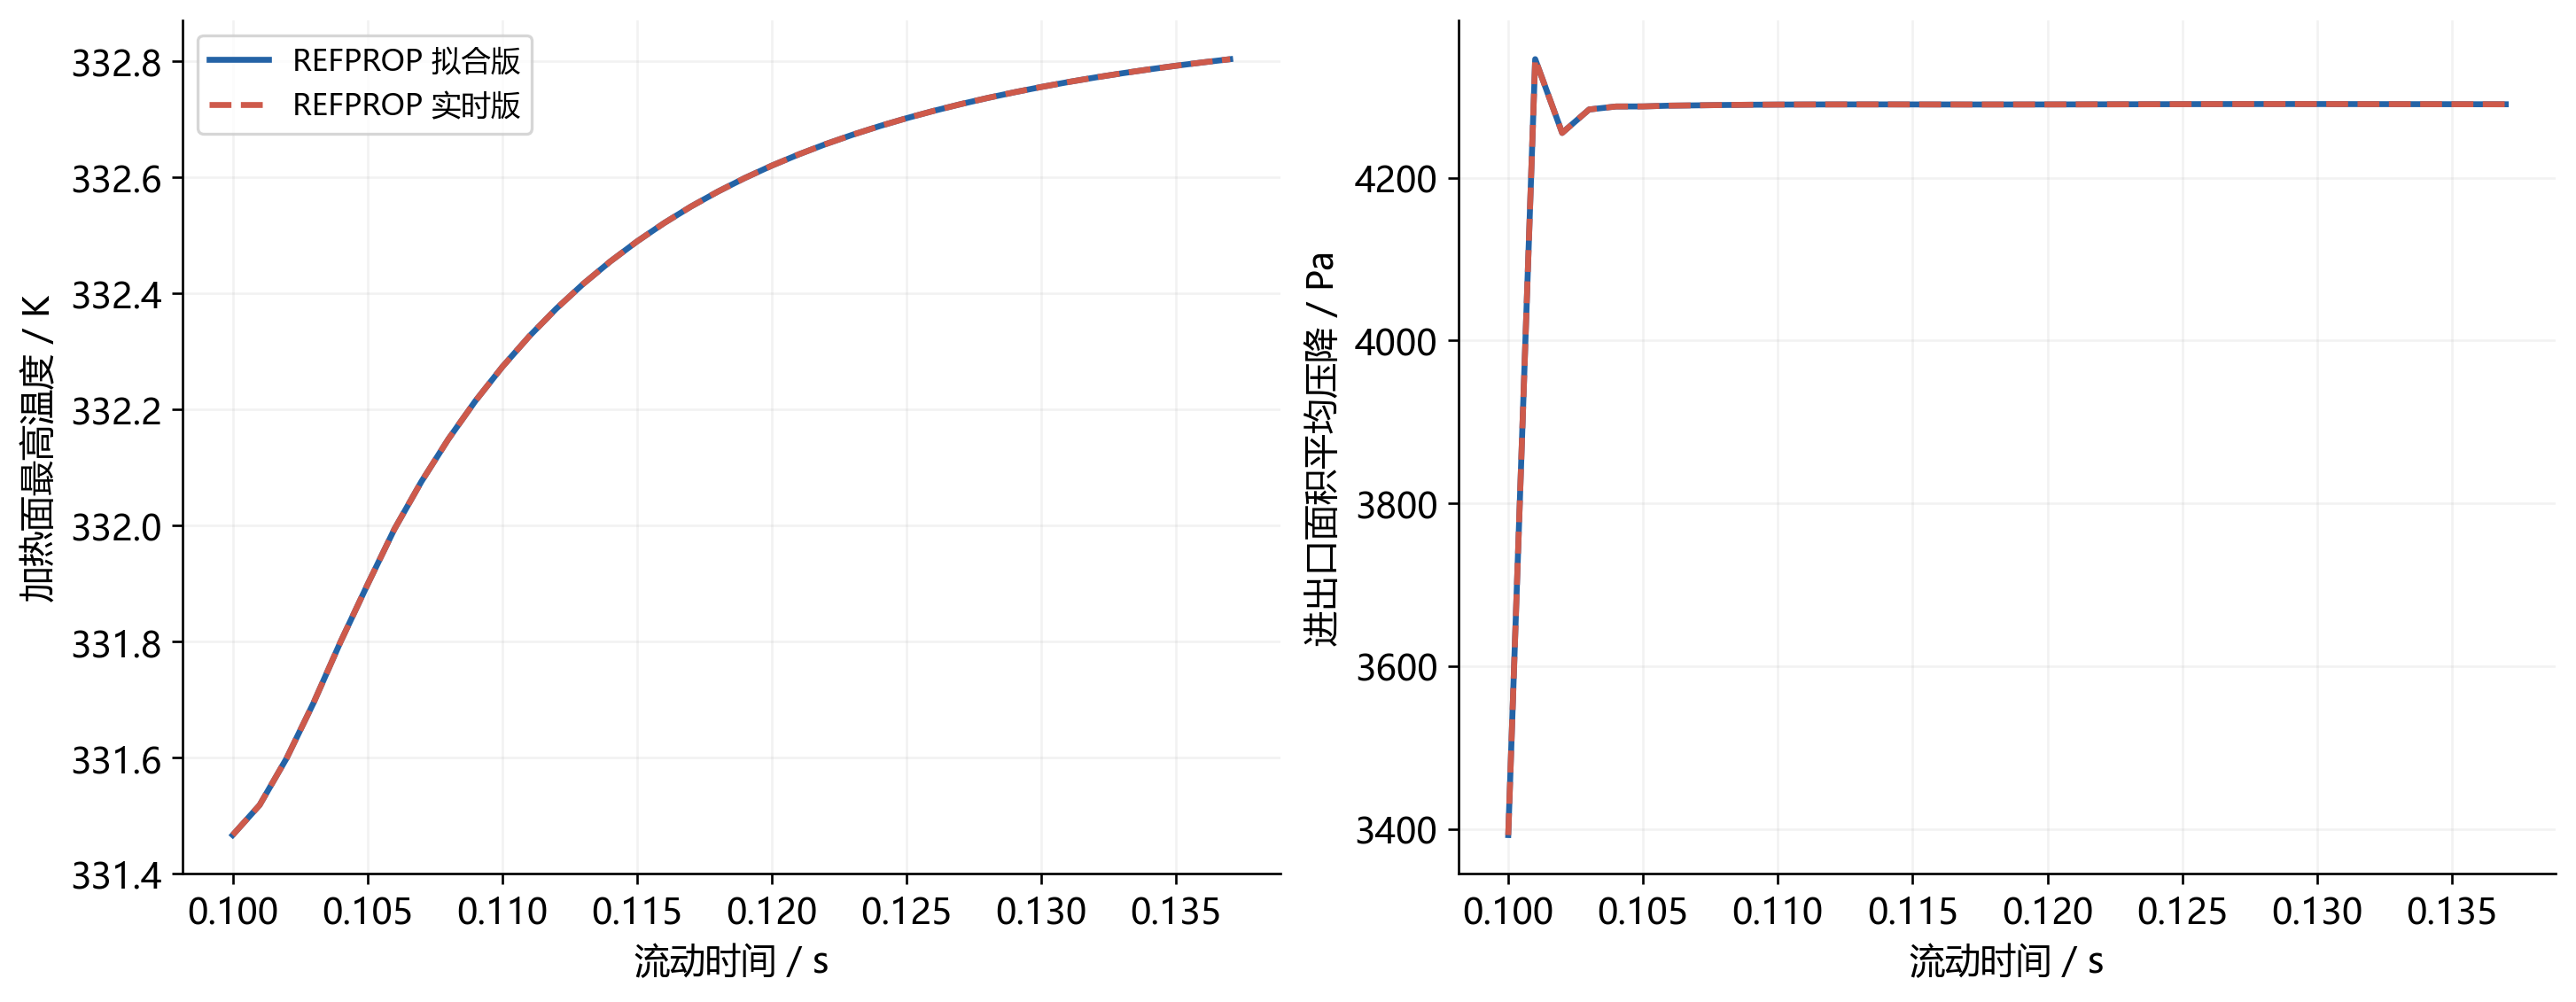
\includegraphics[width=\linewidth]{figs/midterm_asset_udf_04_同一时段求解结果.png}
\caption{相同初场和时间步下两种物性实现的共同时间段对照。}\label{fig:udf-common}
\end{subfigure}\hfill
\begin{subfigure}{0.49\linewidth}\centering
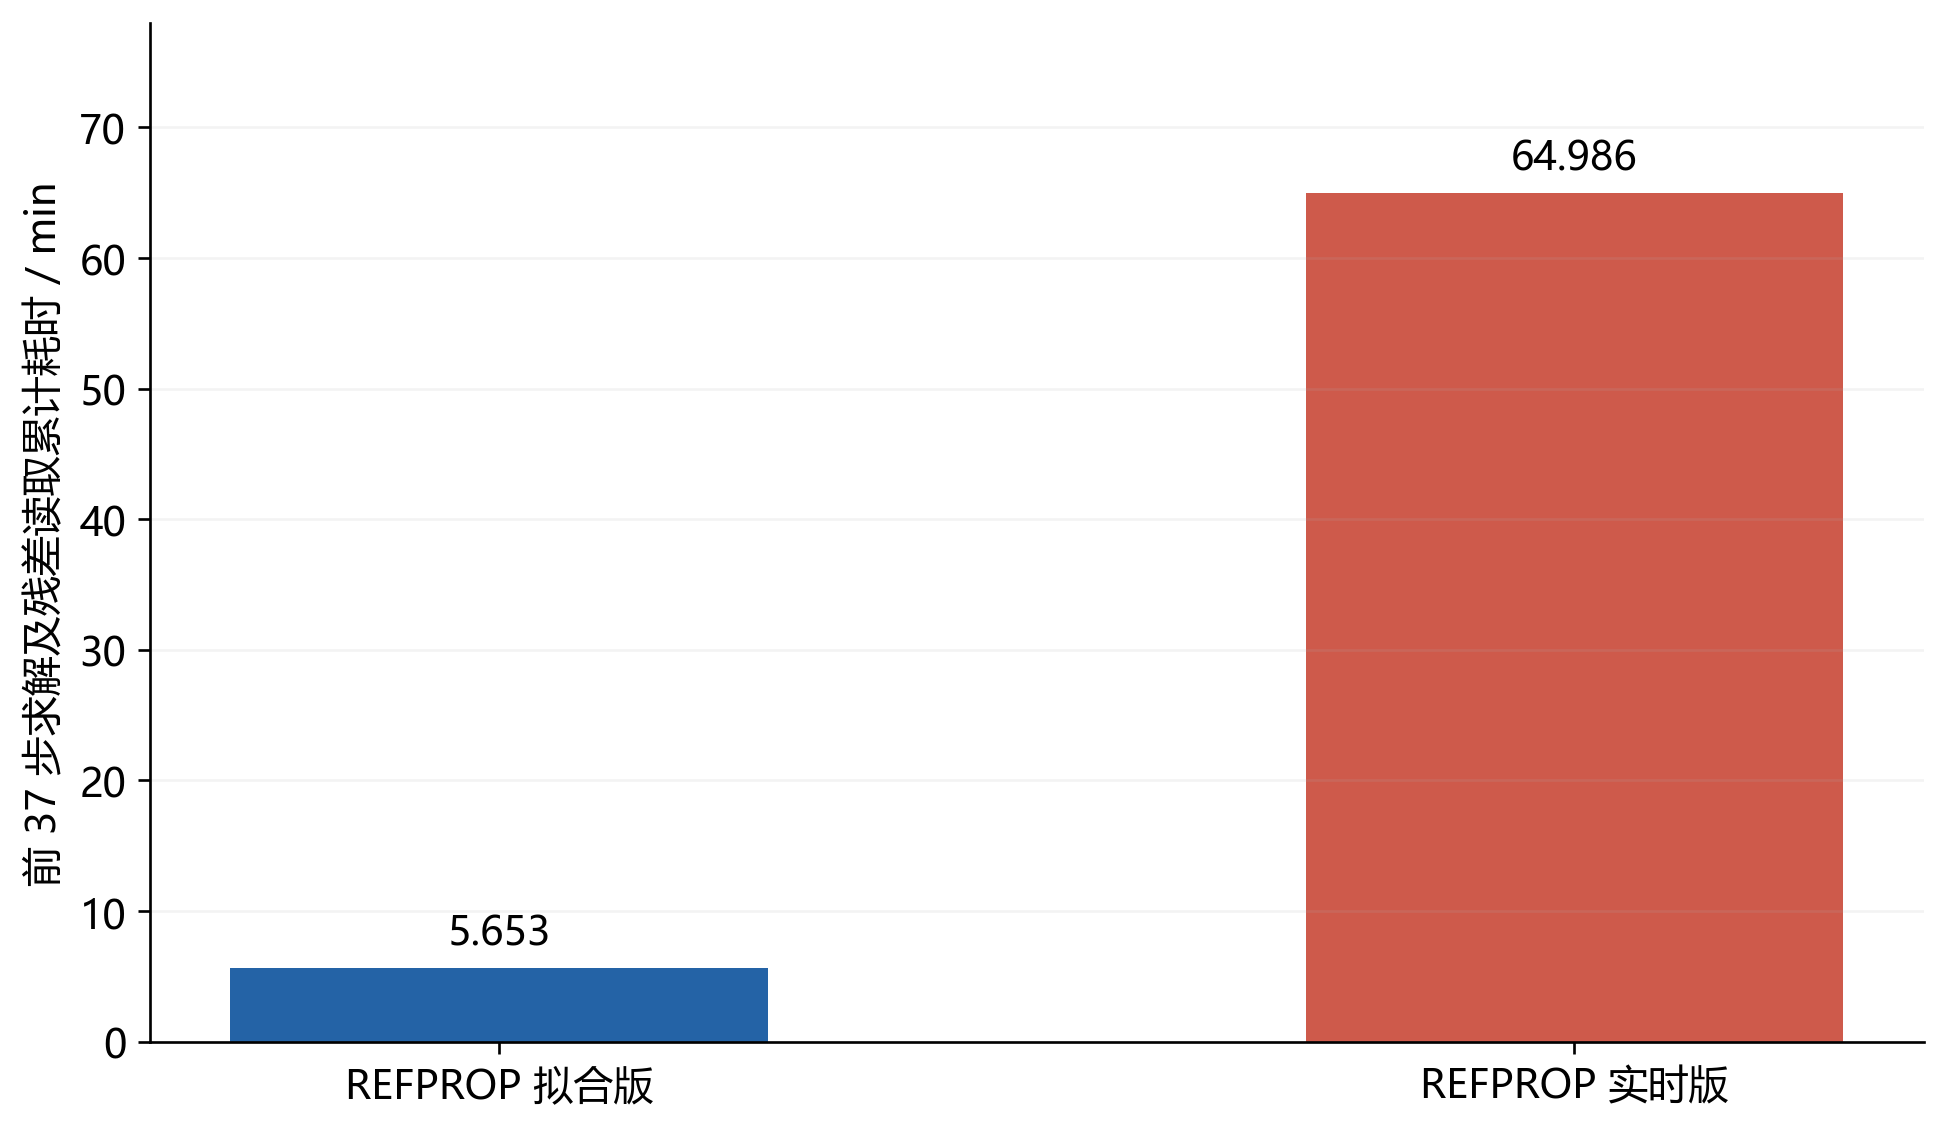
\includegraphics[width=\linewidth]{figs/midterm_asset_udf_05_共同37步计算耗时.png}
\caption{共同前37步的求解及残差读取耗时；不是不同总步数或代理模型的加速比较。}\label{fig:udf-time}
\end{subfigure}
\caption{两种物性实现的求解结果与计算耗时}
\end{figure}

\FloatBarrier

\subsection{方向一：结构对照结果}
结构对照按对象分组：共同热流密度下的四种流道、其他小模型、六种翼型基准和 NACA 小模型分支。各表的平均温度定义、保存时刻与流量条件均在表内注明，不同口径之间不直接横向排序。
\subsubsection{四种流道在共同热流密度下的比较}

表~\ref{m2:tab:results}列出既有工况下的最高温度、平均温度、压差与水力功率。
\begin{table}[!htbp]
\centering
\caption{既有工况在共同热流密度下的温度与水力性能}
\label{m2:tab:results}
\begin{tabularx}{\textwidth}{@{}c Y Y Y Y Y@{}}
\toprule
\rowcolor{ydzjlight} 热流密度 & 流道 & 最高温度 & 平均温度 & 压差 & 水力功率 \\
 & & / $^\circ$C & / $^\circ$C & / kPa & / W \\
\midrule
300 & 直线 & 52.50 & 38.43 & 3.074 & 0.04919 \\
300 & 正弦 & 62.27 & 44.84 & 4.914 & 0.05897 \\
300 & NACA2416 & 72.48 & 45.99 & 0.979 & 0.01566 \\
500 & gao2.1 & 68.50 & 42.55 & 12.457 & 0.11211 \\
500 & NACA2416 & 99.60 & 56.82 & 0.926 & 0.01482 \\
\bottomrule
\end{tabularx}
\end{table}

在 150 至 300 W/cm$^2$ 的共同工况下，最高温度与平均温度均为
直线低于正弦、正弦低于 NACA2416；
压差与水力功率则为 NACA2416 低于直线、直线低于正弦。

300 W/cm$^2$ 时，直线最高温度比正弦低 9.77 $^\circ$C，比 NACA2416 低 19.98 $^\circ$C；
相对正弦，其压差低约 37.4\%，水力功率低约 16.6\%。
NACA2416 的压差与水力功率均比直线低约 68.2\%，但最高温度较高。


\subsubsection{流道形态与网格的补充}
在既有四种流道数据之外，团队补充整理了六边形 v4、六边形 v4.2、
gao2.1 和叶脉 A\_leaf 的保存结果。表~\ref{m2:tab:other-small} 记录了各自工况下的
温度和水力指标，表~\ref{m2:tab:other-conditions} 列出网格与计算条件。
其中叶脉模型已经完成建模并保存了稳态结果，可作为后续仿生结构筛选的基础。

本次新增表格的平均温度统一采用\textbf{固体单元温度算术平均}，
与前表既有数据中的体积平均温度、后续翼型表中的底板平均温度分别保留；
最高温度取固体单元最大值，压差取入口与出口的面积加权平均静压之差，
水力功率按 $P_{\mathrm{hyd}}=\Delta p\,\dot V$ 计算。
对于 gao2.1 的多个入口和出口，分别按总面积加权，入口体积流量取各入口之和。
\begin{table}[!htbp]
\centering
\small
\caption{非 NACA 小模型在各自保存工况下的性能}
\label{m2:tab:other-small}
\begin{tabularx}{\textwidth}{@{}Y r r r r r@{}}
\toprule
\rowcolor{ydzjlight} 模型或分支 & 热流密度 & 最高温度 & 平均温度 & 压差 & 水力功率 \\
 & / (W/cm$^2$) & / $^\circ$C & / $^\circ$C & / kPa & / W \\
\midrule
六边形 v4 & 350.00 & 45.75 & 30.77 & 512.097 & 39.45329 \\
六边形 v4.2 & 650.00 & 88.26 & 49.50 & 78.587 & 1.17881 \\
gao2.1 & 600.00 & 88.41 & 53.57 & 13.969 & 0.12572 \\
叶脉 A\_leaf & 600.00 & 61.81 & 37.92 & 47.668 & 0.76269 \\
\bottomrule
\end{tabularx}
\end{table}

\begin{table}[!htbp]
\centering
\small
\caption{非 NACA 小模型的网格与计算条件}
\label{m2:tab:other-conditions}
\begin{tabularx}{\textwidth}{@{}Y r r r r@{}}
\toprule
\rowcolor{ydzjlight} 模型 & 网格单元数 & 保存时刻 / s & 时间步 / s & 流量 / (mL/s) \\
\midrule
六边形 v4 & 1,443,844 & 15.00 & 0.5 & 77.043 \\
六边形 v4.2 & 1,320,229 & 6.05 & 0.01 & 15.000 \\
gao2.1 & 2,347,198 & 0.20 & 0.01 & 9.000 \\
叶脉 A\_leaf & 5,031,324 & 稳态 & --- & 16.000 \\
\bottomrule
\end{tabularx}
\end{table}

六边形 v4 与 v4.2 的热负荷和流量同时发生变化，因此不能把两者的温度差
解释为结构优化的净收益。gao2.1 与叶脉模型虽然都采用 600 W/cm$^2$，
但流量分别为 9 和 16 mL/s，且一个是瞬态保存结果、一个是稳态结果；
当前只能记录各自的散热表现与水力代价，尚不能据此给出结构优劣排序。

图~\ref{m2:fig:other-small} 对照展示了三种代表模型的流固界面网格和加热面温度。
图中网格来自实际 Case 文件的平面界面面元，温度直接读取配套 Data 文件的加热面数据，
没有额外推进求解。各温度子图采用独立色标，颜色仅反映各自工况的温度分布。
现有单元数可说明离散规模，\textbf{不能仅据此认定网格无关性已经通过}；
仍需对同一几何在统一工况和收敛标准下比较不同网格的结果。

\begin{figure}[!htbp]
\centering
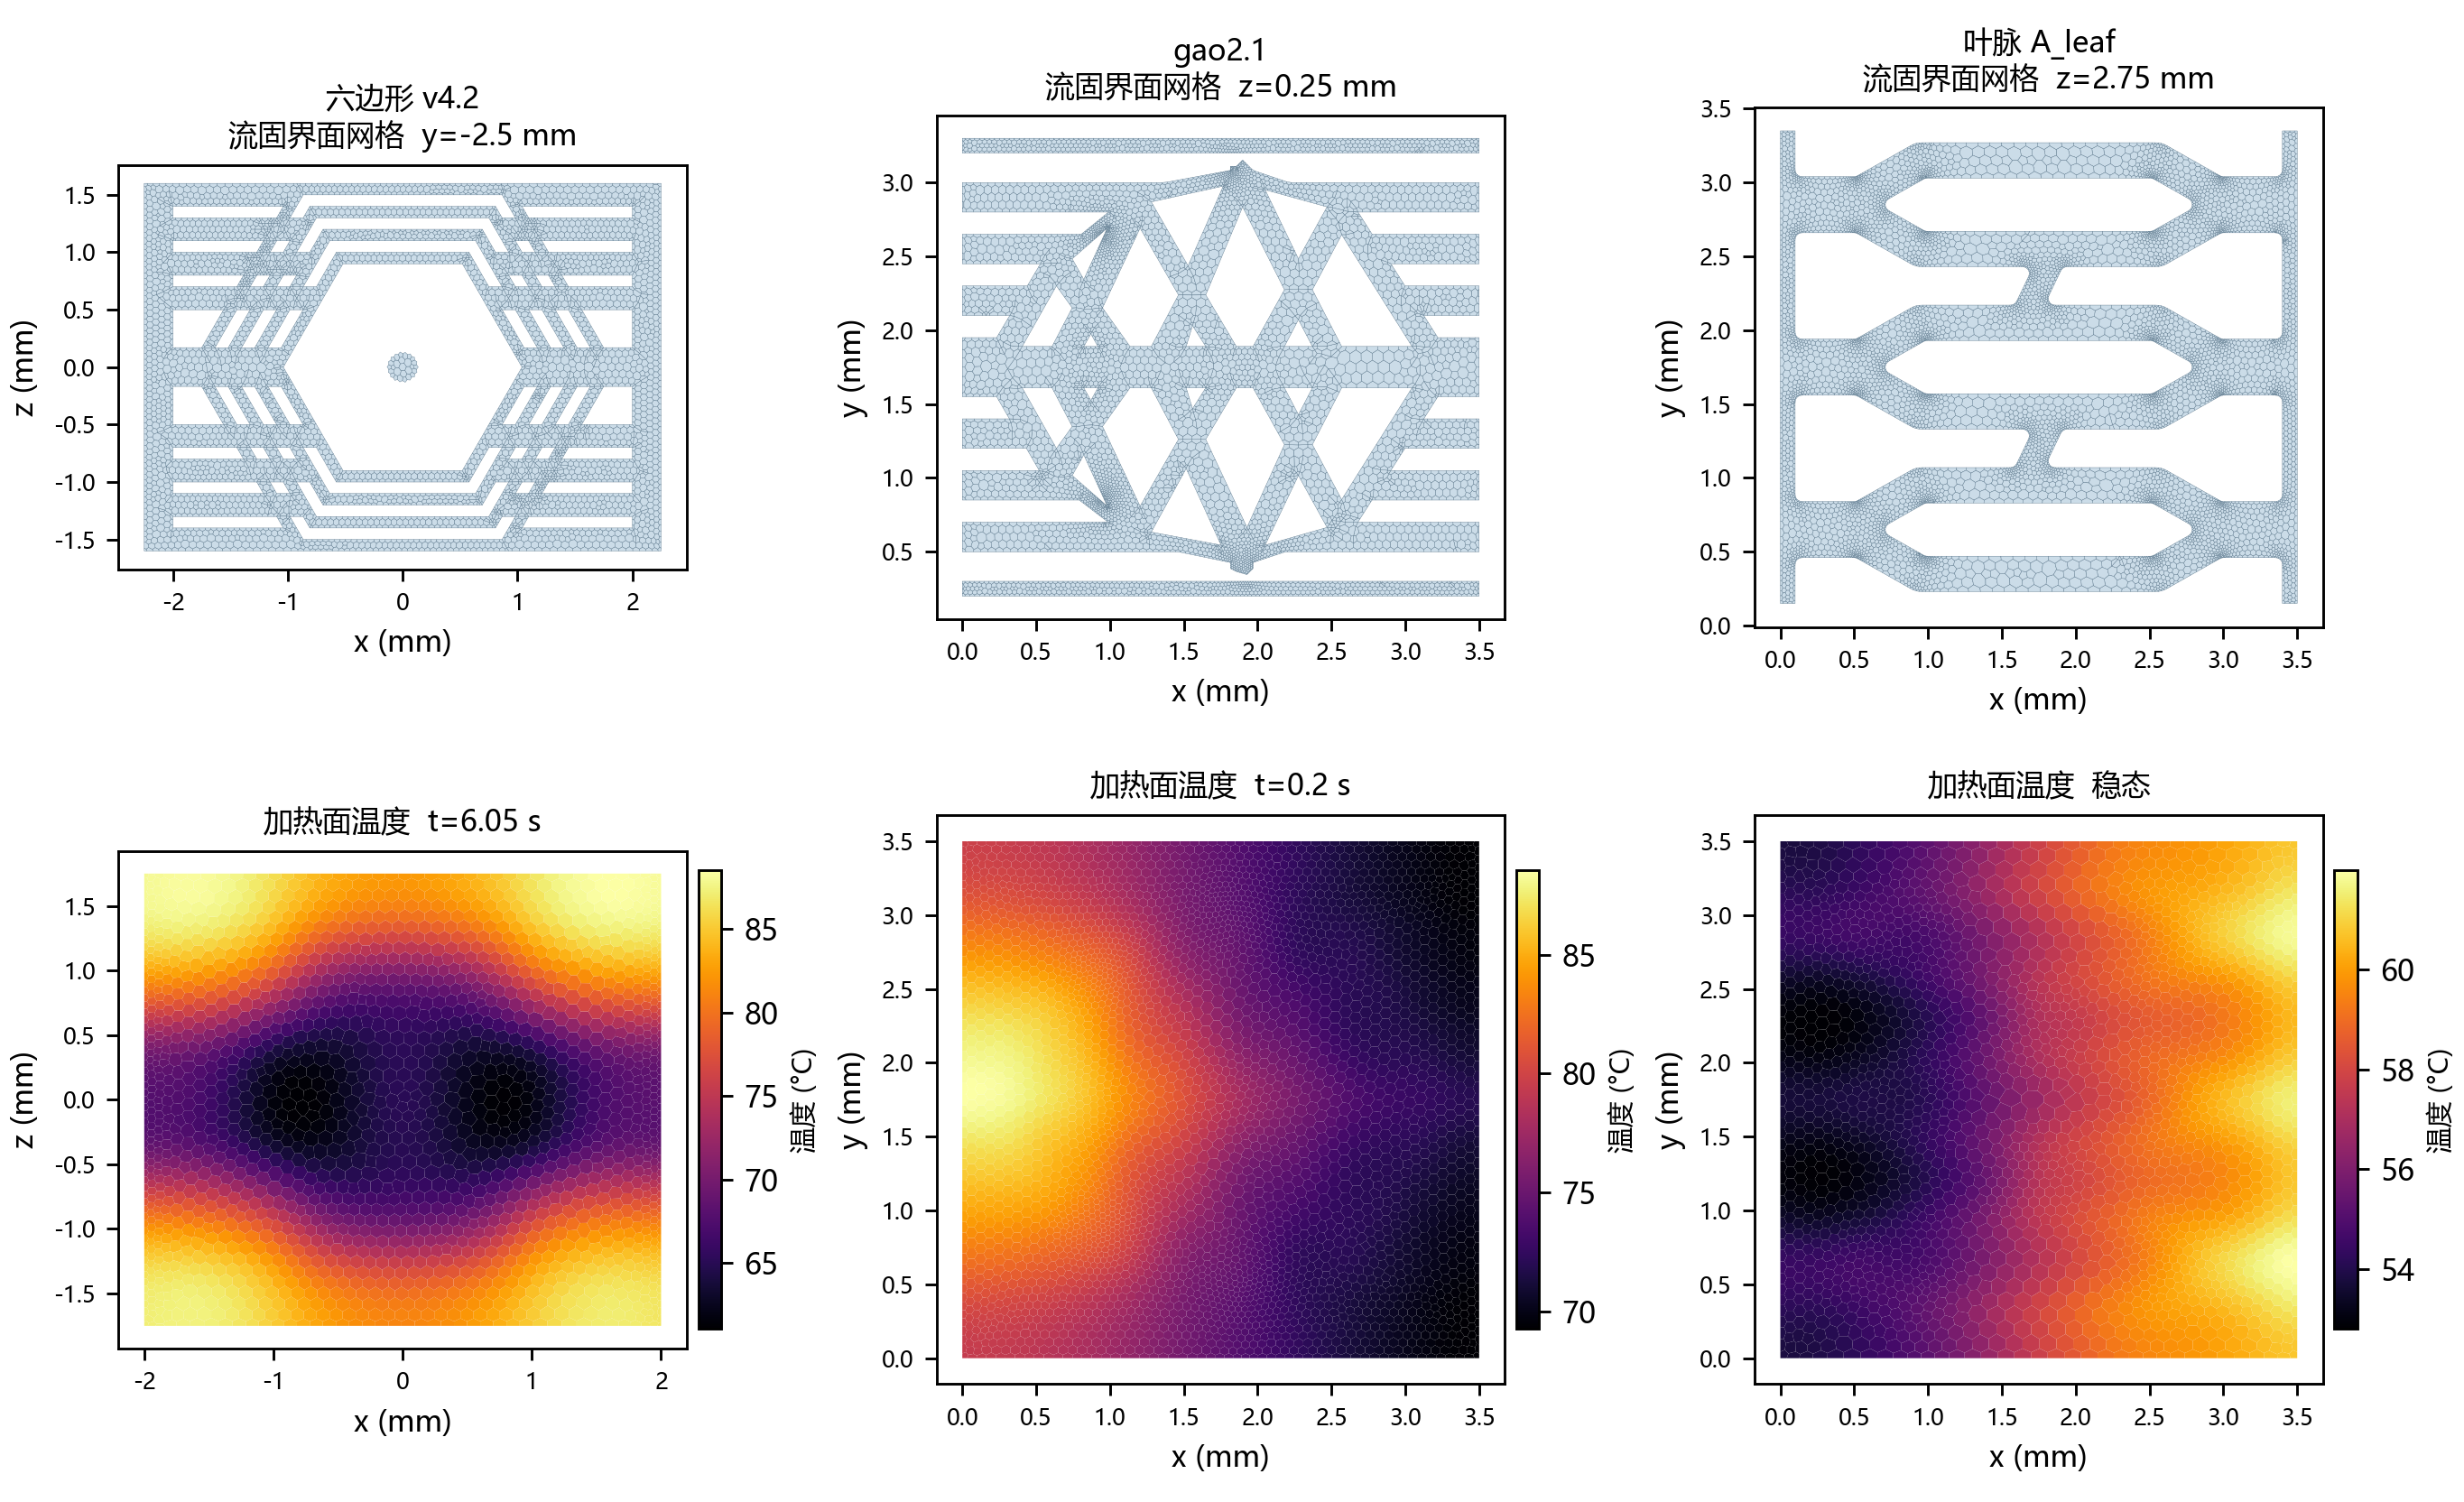
\includegraphics[width=\textwidth]{figs/midterm_month2_other_models.png}
\caption{六边形 v4.2、gao2.1 与叶脉模型的实际界面网格及加热面温度。上排为平面流固界面网格，下排为各自保存工况的加热面温度；各列工况不同，色标独立。}
\label{m2:fig:other-small}
\end{figure}


\subsubsection{六种翼型在基准工况下的比较}

\begin{table}[!htbp]
\centering
\caption{不同翼型构型流热耦合仿真关键结果（基准工况）}
\label{m2:tab:airfoil}
\begin{tabularx}{\textwidth}{@{}l c c c c@{}}
\toprule
\rowcolor{ydzjlight} 构型 & 最高温度 / K & 底板平均温度 / K & $h$ / (W/(m$^2$·K)) & PEC \\
\midrule
NACA0015 & 357.9 & 356.1 & 756.6 & 1.00 \\
NACA0021 & 355.7 & 354.0 & 765.3 & 1.10 \\
NACA0024 & 354.9 & 353.2 & 798.5 & 1.19 \\
NACA4424 & 354.4 & 352.7 & 789.8 & 1.21 \\
NACA6424 & 358.1 & 356.3 & 750.5 & 1.00 \\
NACA6624 & 357.9 & 356.1 & 750.2 & 1.01 \\
\bottomrule
\end{tabularx}
\end{table}

PEC 以 NACA0015 为基准归一化。厚度增益符合预期：
NACA0015 增至 NACA0024 后最高温度由 357.9 K 降至 354.9 K，
表列换热系数由756.6增至798.5 W/(m$^2$·K)，提高约5.54\%。弯度效应与预期存在偏差：
NACA64 系列 PEC 反而回落至 1.00 附近。


\subsubsection{NACA 分支结果}
在上述六种翼型基准对比之外，团队进一步整理了 NACA0016、1416、2416、3416
及 2420 的已有小模型结果，共 13 条代表性分支。
这些分支包含几何变化、网格组织、物性验证及时间步验证，不能全部视为独立翼型。
新增表格沿用前述固体单元算术平均温度和水力功率口径，不将其平均温度
直接并入表~\ref{m2:tab:airfoil} 的底板平均温度，也不据此补算缺少统一基准的 PEC。

\paragraph{350 W/cm$^2$ 下的几何、网格与物性分支}
表~\ref{m2:tab:naca350} 中各分支的入口体积流量均约为 16 mL/s。
L450 表示弦长 450 $\mu$m，A06 与 A00 分别对应 $6^\circ$ 和 $0^\circ$ 攻角，
原模型目录中的 98989 阵列标识保留在数据来源中。
NACA0016 A06 基础分支为 3,048,985 单元，保存时刻 0.10 s；
其拟合物性和 REFPROP 物性分支采用相同网格，时间步均为 0.001 s，
但分别保存于 0.200 s 和 0.137 s。
NACA2416 A00 core 与尾部 BOI 分支分别为 4,371,445 和 3,079,413 单元，
保存时刻分别为 0.15 s 和 0.20 s，时间步均为 0.01 s；
NACA2416 v3 列出 3,235,081 单元、时间步 0.001 s、0.20 s 时刻的结果。
基础 NACA0016 A06 的时间步为 0.01 s。
\begin{table}[!htbp]
\centering
\small
\caption{350 W/cm$^2$ 下 NACA 小模型的保存结果}
\label{m2:tab:naca350}
\begin{tabularx}{\textwidth}{@{}Y r r r r r@{}}
\toprule
\rowcolor{ydzjlight} 模型或分支 & 热流密度 & 最高温度 & 平均温度 & 压差 & 水力功率 \\
 & / (W/cm$^2$) & / $^\circ$C & / $^\circ$C & / kPa & / W \\
\midrule
0016 A06 基础 & 350.00 & 58.20 & 34.18 & 3.393 & 0.05428 \\
2416 A00 core & 350.00 & 71.03 & 40.07 & 2.456 & 0.03929 \\
2416 A00 尾部 BOI & 350.00 & 71.01 & 39.25 & 2.512 & 0.04019 \\
0016 A06 拟合物性 & 350.00 & 59.61 & 34.62 & 4.290 & 0.06864 \\
0016 A06 REFPROP & 350.00 & 59.54 & 34.59 & 4.290 & 0.06864 \\
2416 v3 & 350.00 & 72.83 & 38.74 & 2.348 & 0.03757 \\
\bottomrule
\end{tabularx}
\end{table}

这些记录说明了不同分支的温度与水力量级，但保存时刻、攻角及网格并未全部一致。
尤其是物性分支的最终保存时刻不同，不能用本表的末态温差代替同一时刻的物性误差；
core 与 BOI 分支也不能仅凭本表认定网格无关。

\paragraph{450 W/cm$^2$ 下三种 v2 翼型的初步比较}
三组结果的热流密度均为 450 W/cm$^2$，入口流量约为 16 mL/s，
时间步均为 0.0002 s，保存时刻均为 0.10 s。
NACA0016、1416、3416 的网格分别为 821,987、792,259、783,184 单元。
表~\ref{m2:tab:nacav2} 显示，三者最高温度相差不足 0.23 $^\circ$C；
与 NACA0016 相比，NACA3416 最高温度降低约 0.230 $^\circ$C，
压差和水力功率均提高约 5.25\%。
这提示弯度变化带来的温度收益需要与流动代价一起衡量，
但当前数据只支持该保存时刻的初步比较，仍需检查收敛状态和网格敏感性。
\begin{table}[!htbp]
\centering
\small
\caption{同热负荷、同流量与同保存时刻的 v2 翼型结果}
\label{m2:tab:nacav2}
\begin{tabularx}{\textwidth}{@{}Y r r r r r@{}}
\toprule
\rowcolor{ydzjlight} 模型或分支 & 热流密度 & 最高温度 & 平均温度 & 压差 & 水力功率 \\
 & / (W/cm$^2$) & / $^\circ$C & / $^\circ$C & / kPa & / W \\
\midrule
NACA0016 v2 & 450.00 & 85.34 & 43.21 & 2.248 & 0.03596 \\
NACA1416 v2 & 450.00 & 85.31 & 43.46 & 2.255 & 0.03609 \\
NACA3416 v2 & 450.00 & 85.11 & 43.12 & 2.366 & 0.03785 \\
\bottomrule
\end{tabularx}
\end{table}

图~\ref{m2:fig:naca-small} 给出了三种 v2 翼型的实际界面网格和加热面温度。
各子图分别标注色标；加热面温度是表面局部值，
与表中固体全域最高温度和固体单元算术平均温度含义不同。

\begin{figure}[!htbp]
\centering
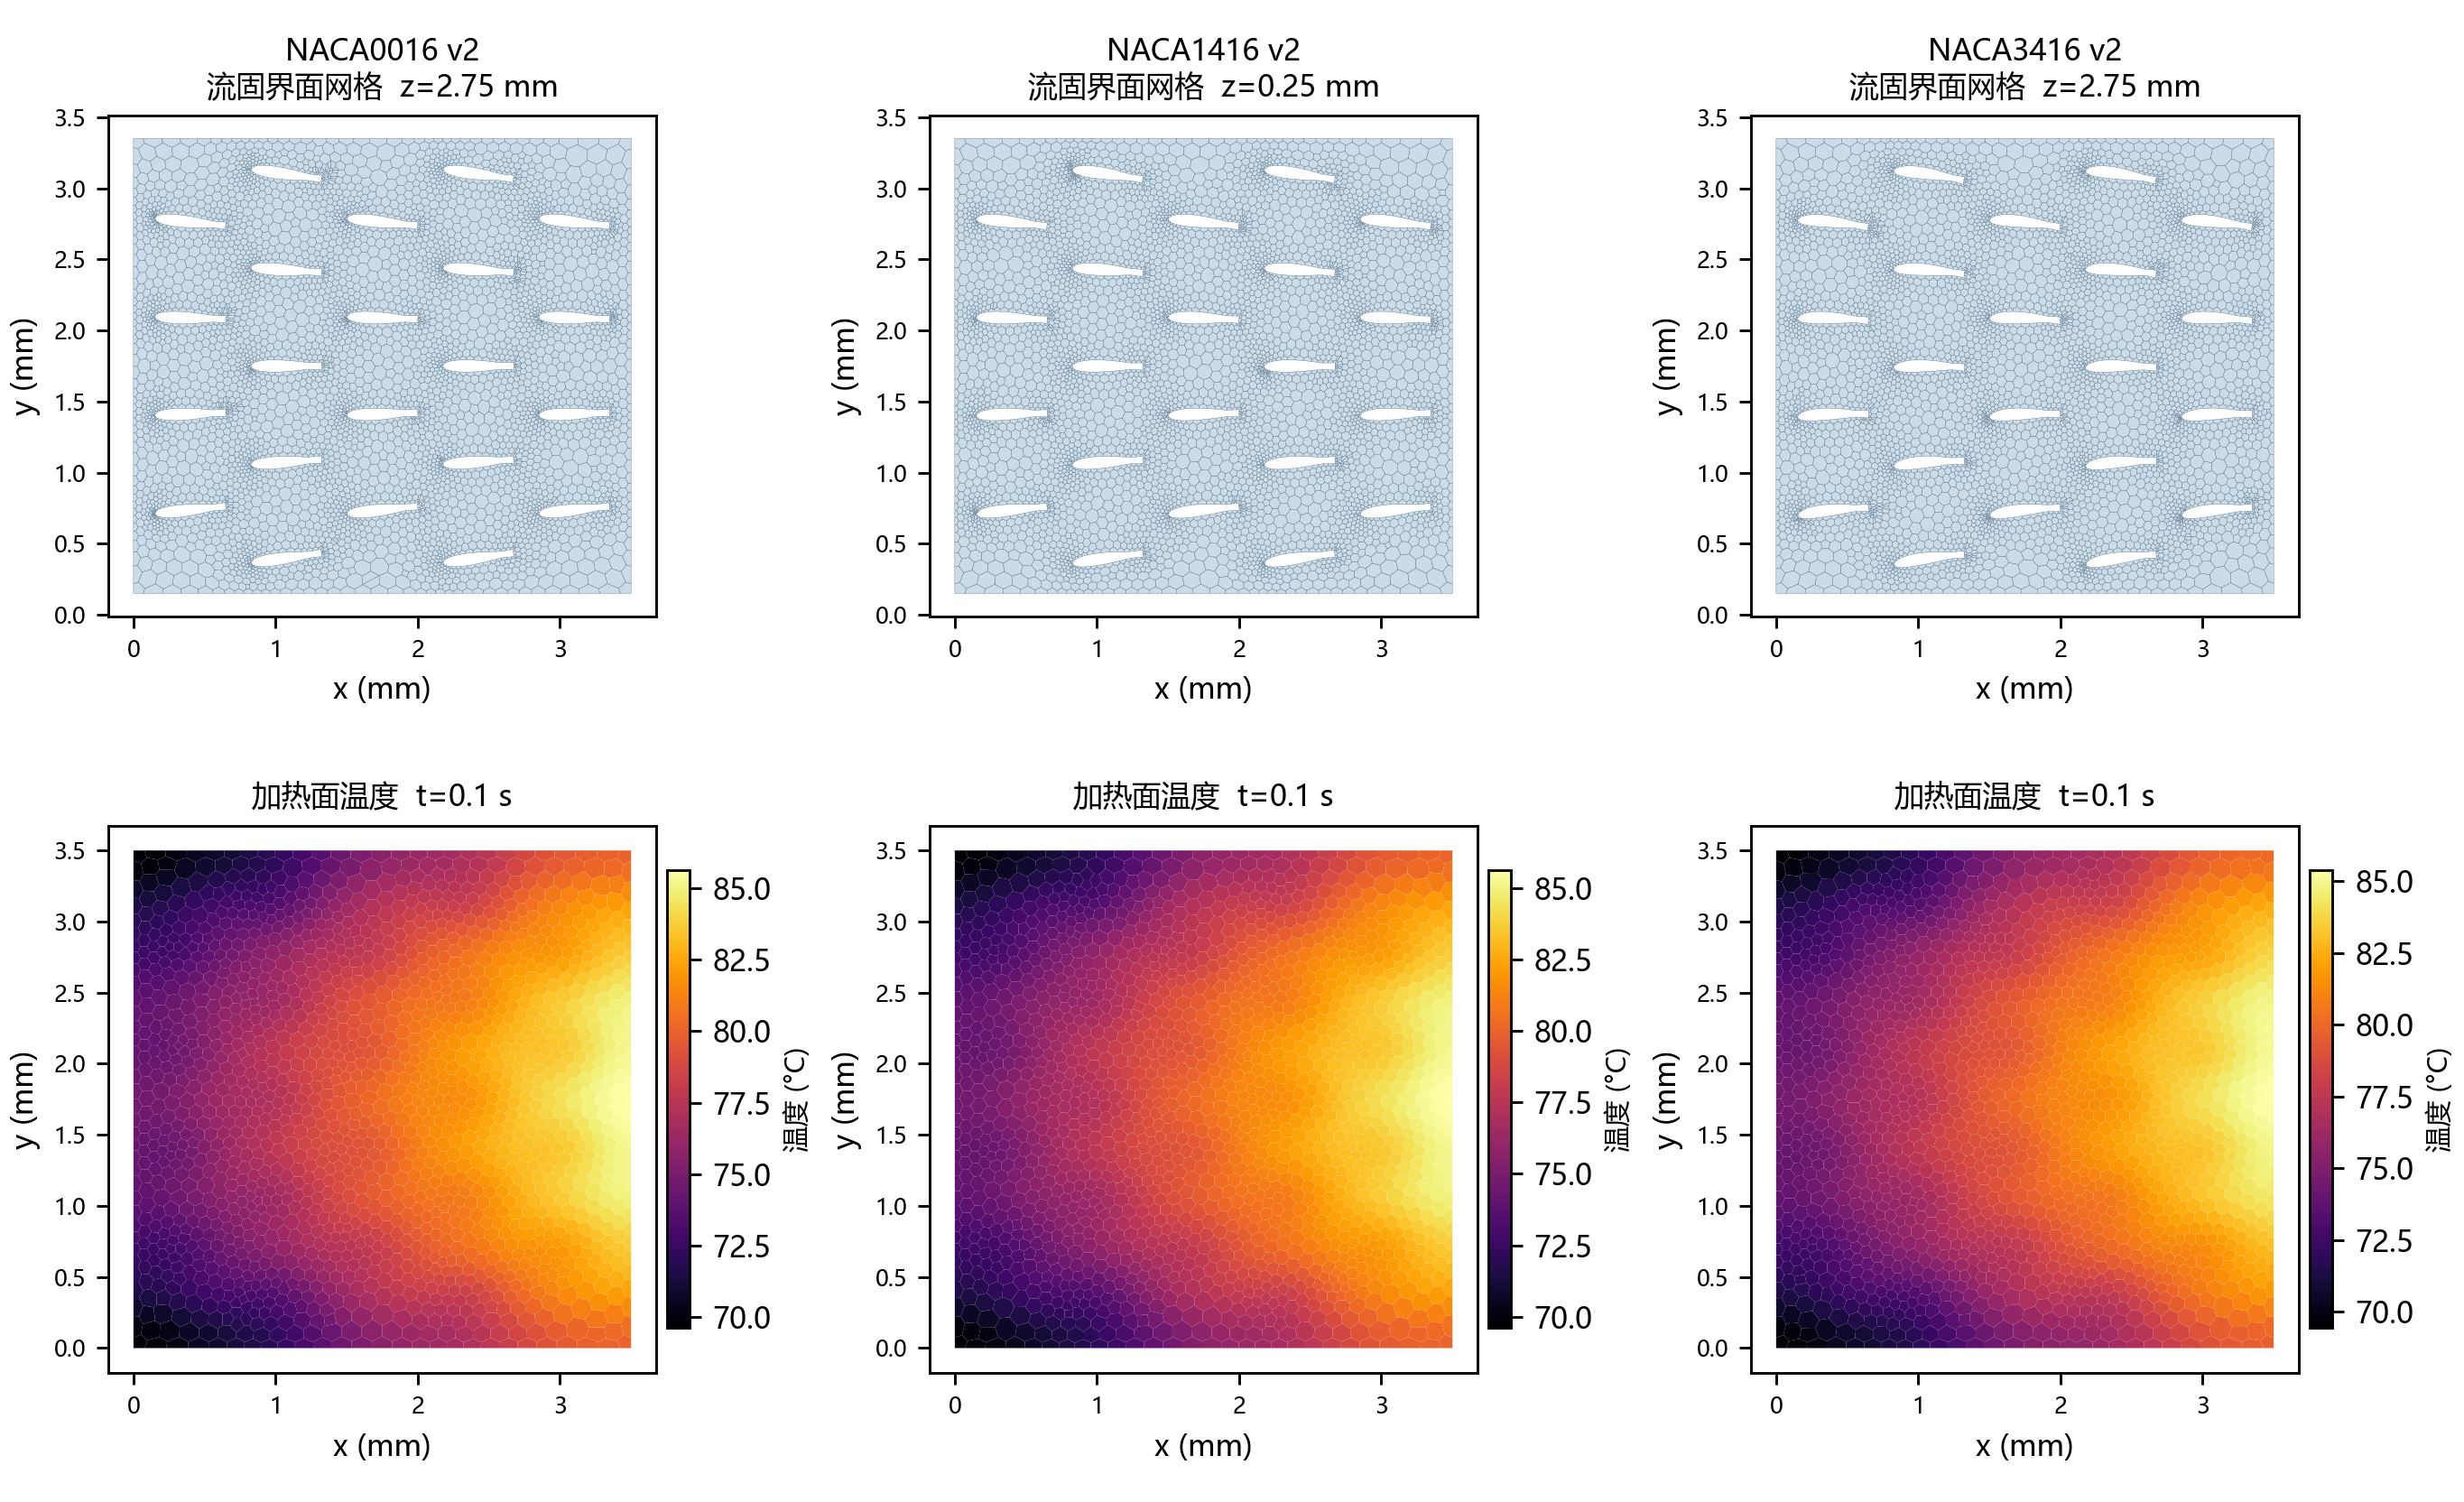
\includegraphics[width=\textwidth]{figs/midterm_month2_naca_models.png}
\caption{NACA0016、1416、3416 v2 小模型的界面网格与 0.10 s 加热面温度。上排为实际平面流固界面网格，下排温度来自各自配套 Data 文件，色标独立。}
\label{m2:fig:naca-small}
\end{figure}

\paragraph{NACA2420 的回流设置、物性与时间步检查}
表~\ref{m2:tab:naca2420} 的四个分支均为 771,225 单元，保存时刻均为 1 s。
加热边界采用随时间变化的热流，表中 126.82 W/cm$^2$ 为 1 s 的瞬时值，
不是整个计算过程的恒定热负荷。原始分支流量约为 12.000 mL/s，
其余三个分支约为 12.041 mL/s；原始与回流温度 300 K 分支的时间步均为 0.01 s。
\begin{table}[!htbp]
\centering
\small
\caption{NACA2420 在 1 s 时刻的设置与时间步验证结果}
\label{m2:tab:naca2420}
\begin{tabularx}{\textwidth}{@{}Y r r r r r@{}}
\toprule
\rowcolor{ydzjlight} 模型或分支 & 热流密度 & 最高温度 & 平均温度 & 压差 & 水力功率 \\
 & / (W/cm$^2$) & / $^\circ$C & / $^\circ$C & / kPa & / W \\
\midrule
2420 v4 原始 & 126.82 & 43.08 & 31.40 & 1.377 & 0.01653 \\
2420 回流 300 K & 126.82 & 44.23 & 31.83 & 1.651 & 0.01988 \\
2420 IAPWS $\Delta t=0.01$ s & 126.82 & 44.32 & 31.87 & 1.652 & 0.01989 \\
2420 IAPWS $\Delta t=0.005$ s & 126.82 & 44.32 & 31.87 & 1.652 & 0.01989 \\
\bottomrule
\end{tabularx}
\end{table}

采用 IAPWS 物性后，将时间步从 0.01 s 减小到 0.005 s，
1 s 时刻的最高温度差约为 $3.68\times10^{-6}$ K，压差相对差约为
$2.75\times10^{-5}\%$，各项指标在表中精度下相同。
因此，这组结果在该时刻对本次时间步减半不敏感；
这一检查不等同于验证整个瞬态过程，也不能替代网格无关性检验。
17条代表结果与源文件对应关系已保留在配套数据中\cite{stagereports}。


上述结果不能转写为连接导叶的性能收益。后续先固定热负荷、入口流量或泵功、物性和统计时刻，
再比较温度与压降；同一模型的网格、物性和时间步分支保留为验证记录，不重复计为新几何样本。
\FloatBarrier
\subsubsection{阶段小结}

方向一已积累四种流道与六种翼型的基准对照、17条小模型分支，以及可追溯的条带与整板装配几何。
局部数据支持温度收益与水力代价之间的权衡判断，但连接段本身尚无成对结果，装配几何也不等于系统性能。
40 mm条带和整板装配只提供计算输入，不能代替系统计算。


\FloatBarrier

\subsection{方向二：闭环仿真结果}
方向二的量化结果来自简化闭环时序及其程序复核，尚不包括真实泵阀系统。下面先给出保存的时序，再说明程序核查发现的问题。
图~\ref{fig:20}直接由已有数组重绘，表~\ref{tab:11}按明确统计窗口复核\cite{stagereports}。

\begin{figure}[!htbp]\centering
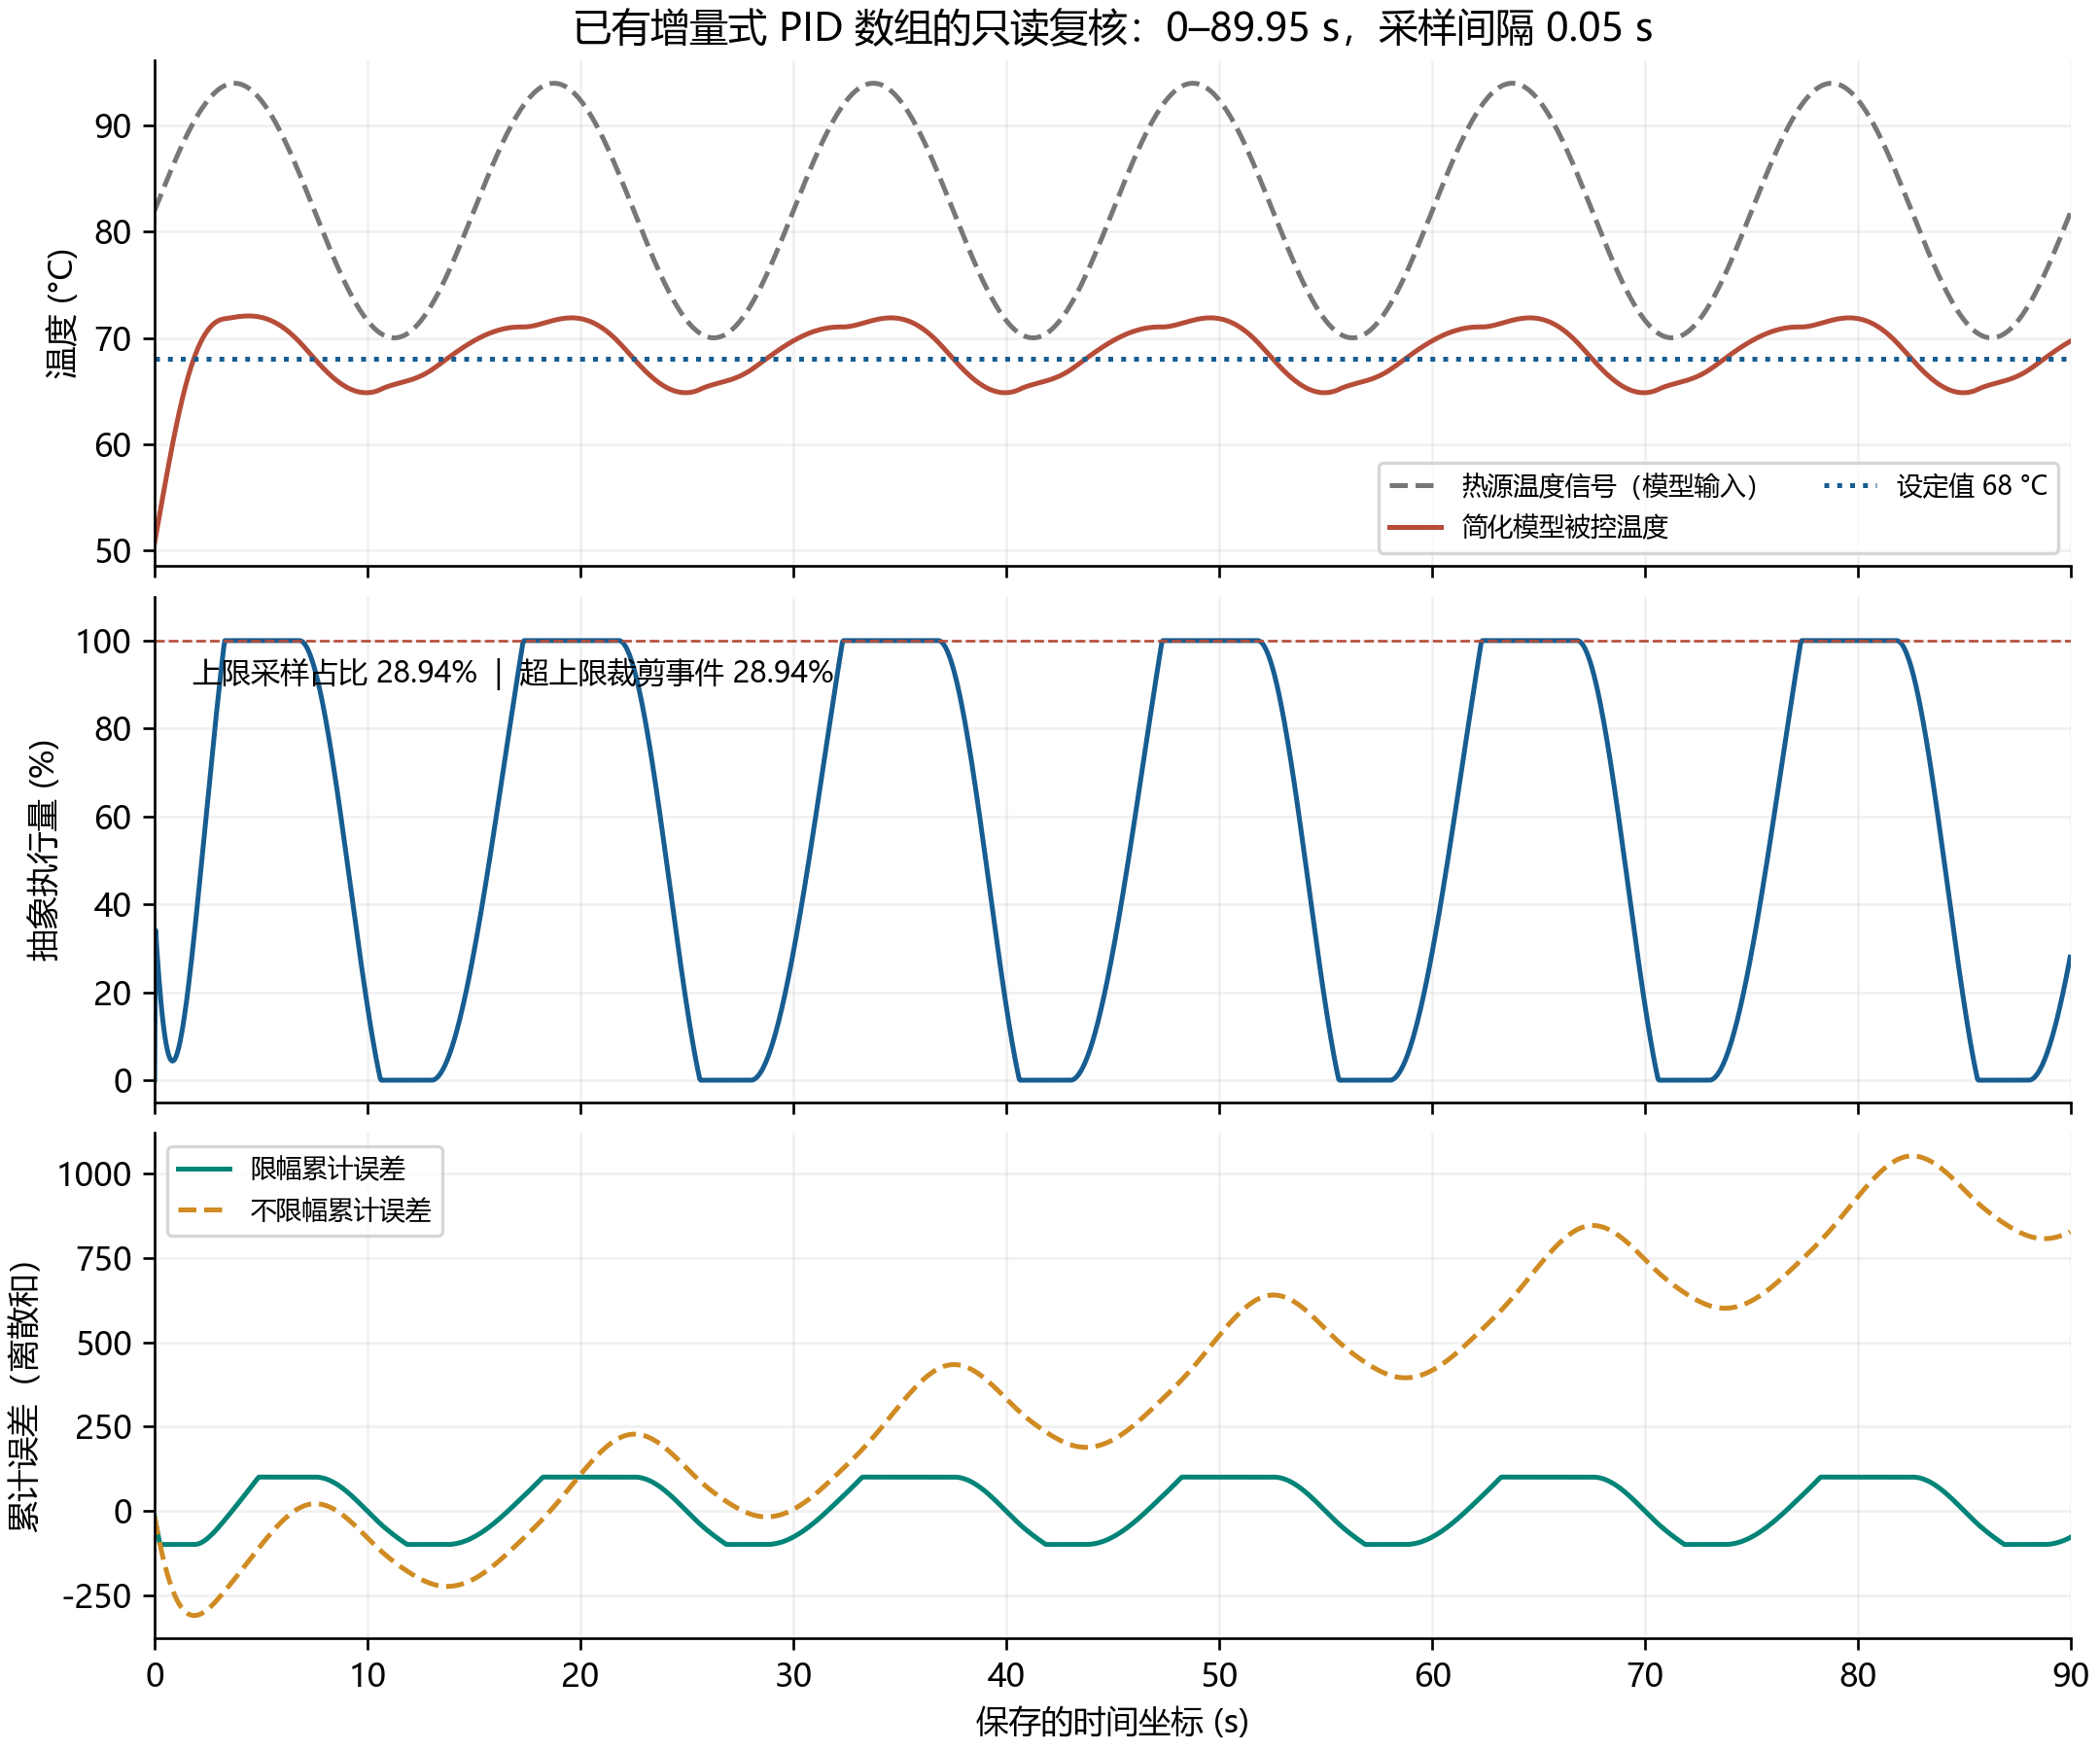
\includegraphics[width=.9\linewidth,height=150mm,keepaspectratio]{figs/midterm_asset_pid_verified.png}
\caption{已有简化 PID 温控数组的只读复核。上图为温度扰动与被控温度，中图为限幅执行量，下图为开关累计误差限幅时的累计值；不表示实物流量。}\label{fig:20}
\end{figure}

\begin{table}[!htbp]\centering\small
\caption{保存 PID 时序的工况与复核指标}\label{tab:11}
\begin{tabularx}{\linewidth}{@{}Y Y Y@{}}\toprule
\rowcolor{ydzjlight} 项目 & 数值或状态 & 统计与适用范围 \\\midrule
设定值／初始温度 & 68／50 $^\circ$C & 首个保存温度为更新后50.67625 $^\circ$C。\\
离散增益／采样周期 & $K_p=8.0,K_i=0.5,K_d=2.0$；0.05 s & 增量更新的已有参数，不直接等同连续增益。\\
全时段温度范围 & 50.6763--72.0657 $^\circ$C & 相对68 $^\circ$C全时段最大偏高4.0657 K。\\
后半时段峰值偏高 & 3.8865 K & 原记录3.9 K对应后半段45--89.95 s，不是全程峰值。\\
执行量范围与均值 & 0--100\%；均值54.3705\% & 为经验模型抽象动作，未标定为泵速或流量。\\
上限采样占比 & 28.9444\% & 以保存数组 $U\ge100-10^{-10}$ 逐点统计；原记录29.3\%未由当前数组复现。\\
累计误差峰值 & 限幅100；不限幅1052.6016 & 仅记录累计量变化，不能单独证明抗饱和有效。\\
开关限幅后的温度／执行量差 & 两者最大绝对差均为0 & 当前程序没有将该累计量用于增量更新。\\
\bottomrule\end{tabularx}\end{table}
原程序先更新并限幅累计误差变量，随后用当前和前两步误差直接计算增量，未使用被限幅的累计值。
因此两组保存的温度和执行量完全相同，现有结果不能支持“积分限幅已改善超调”的结论。
后续需将抗饱和反馈或条件积分接入实际控制更新，再与相同扰动、初态和模型下的基准比较。
当前峰值仍受经验冷却能力上限影响，但不能据此量化真实泵阀系统的结构性超调或节能收益。

\subsubsection{阶段小结}
方向二已形成十行流路、双泵与行级阀门的架构方案、非均匀热源模型和灰箱模型路线，并保存了简化对象的闭环时序。当前数据不能证明实际泵阀链条已打通，也没有可报告的实际节能效果；辨识、比较与验证安排见下一部分。
\subsection{方向三：方法与数据基础}
方向三已形成参数化建模、自动化批量计算、数据集构建与物理信息融合的技术路线，并完成网格、物性与评价口径的前置整理。代表性翼型建模与仿真、批量 CFD 流程、多轮网格检验和温度相关物性修正，构成了代理模型的数据与数值基础；17条小模型代表分支及37条原始提取记录可用于来源整理，但工况、时刻与物性尚未统一，不能直接视为37个合格训练样本。

翼型参数分组后的 XGBoost 尝试目前尚未开展，参数分组完整数据、训练测试划分及独立结果均待补，因此本方向目前没有可报告的预测精度、泛化能力或计算加速收益。后续按“统一标签—建立基础模型—加入物理信息—消融比较—泛化与成本验证”的顺序推进，具体安排见下一部分。
\FloatBarrier


\subsection{成果清单与结论边界}
本节把前面的进展收拢为表~\ref{tab:monthly_status}（任务状态）、表~\ref{tab:key_results}（量化记录）和一组结论边界。状态按“已有结果—部分完成—未完成”三级描述，不使用完成百分比。

\begin{table}[!htbp]\centering\small
\caption{按现有保存记录核对的中期任务状态}\label{tab:monthly_status}
\begin{tabularx}{\linewidth}{@{}>{\hsize=0.9\hsize}Y c >{\hsize=1.25\hsize}Y >{\hsize=0.85\hsize}Y@{}}
\toprule
\rowcolor{ydzjlight} 方向与任务 & 状态 & 已有证据 & 下一步 \\
\midrule
方向一：局部结构复现与筛选 & 已有结果 & 三类复现云图；四种流道39工况；六翼型及17条小模型分支。 & 统一工况后进入连接对照。 \\
方向一：连接段及流路集成 & 部分完成 & 连接方案库、40 mm 条带与整板装配几何。 & 连接段成对性能计算。 \\
共享平台：物性实现与数值诊断 & 阶段完成 & 1601点拟合核对、0.137 s实现对照、七档网格与出口诊断。 & 新构型网格与守恒准入。 \\
方向二：动态温控原型 & 部分完成 & 1800点简化 PID 时序及程序复核。 & 抗饱和修正与设备辨识。 \\
方向三：物理融合代理模型 & 部分完成 & 技术路线、数值与自动化资料。 & 样本集与独立测试精度。 \\
系统协同：整板与多行验证 & 未完成 & 已有几何和热源映射。 & 流体域、网格、求解及系统对照。 \\
\bottomrule\end{tabularx}
\par\smallskip\begin{minipage}{\linewidth}\footnotesize 不填完成百分比；简化 PID 结果不代表十行泵阀系统已经验证。\end{minipage}
\end{table}
\subsubsection{关键量化结果}

已有量化记录见表~\ref{tab:key_results}；数值来自既有报告、保存数组的只读复核与物性验证资料，本次整理没有推进 Fluent 求解。
\begin{table}[!htbp]\centering\small
\caption{已有量化记录与证据边界}\label{tab:key_results}
\begin{tabularx}{\linewidth}{@{}>{\hsize=0.8\hsize}Y >{\hsize=1.1\hsize}Y >{\hsize=1.1\hsize}Y@{}}\toprule
\rowcolor{ydzjlight} 记录 & 量化信息 & 证据边界 \\\midrule
网格敏感性 & 7 档，260169--4610769 单元，统计时刻 0.2 s & 统一以323万档为比较参考；294万档压降差0.3201\%，461万档4.2751\%。\\
温度相关水物性 & 280--360 K，101325 Pa & 拟合适用范围，不表示任意压力与温度均有效。\\
物性实现对照 & 共同 0.137 s 加热面最高温差约 $3.197\times10^{-6}$ K & 实现一致性核对，不代表模型绝对精度。\\
整板几何 & $40\,\mathrm{mm}\times40\,\mathrm{mm}$，$10\times10$ 单元 & 几何与热源映射已完成，整板流热待验证。\\
静态热源布局 & 低/中/高负荷为 70/27/3 格 & 整格加热 2640 W；仅主体加热 2021.25 W。\\
局部模型整理 & 17条代表分支、37条原始提取记录 & 非17种独立结构；各分支工况、物性和时刻分别标识。\\
简化 PID 时序 & 1800点，0.05 s间隔；全程最高72.0657 $^\circ$C & 温度信号扰动；累计误差限幅未接入控制更新。\\
\bottomrule\end{tabularx}\end{table}




\subsubsection{阶段性结论}
\begin{enumerate}
\item 形成了以空间适配与时间调控为起点的研究框架，并在仿真需求推动下拓展出计算加速方法方向。其价值在于明确了工程对象、动态需求与计算方法之间的关系，使后续研究能够共同服务于同一热管理问题。
\item 整理了四种流道的39个既有工况、六种翼型基准结果和17条小模型代表分支，形成结构筛选的资料基础；连接装配已有几何，但性能优势尚待独立计算。
\item 开展翼型模型、网格敏感性和压力统计核验，修正温度相关水物性并进行实现对照，使数值工作从几何生成逐步进入评价口径与可靠性控制。
\item 读取1800个采样点的简化 PID 温控时序并核查程序，为后续灰箱建模和设备辨识提供起点；保存数据同时暴露了积分限幅未进入控制更新的实现问题。
\item 已有当前整板装配与热源映射验证，支持结构与空间热源的统一配置，但整板流热性能仍须后续求解。
\end{enumerate}

上述成果分别对应研究框架、局部结构、数值方法、控制原型和系统几何准备，证据层级不同。已有资料中的局部物性实现计时属于数值实现改进，网格检验属于可靠性评价，几何装配属于工程准备，均不能替代代理模型精度或系统控制收益。当前没有已提供的论文发表、专利或实测节能成果，本报告不填写此类状态。
\subsubsection{可以确定的}
已有成果可以沿“复现与物性学习—局部结构比较—数值诊断—连接装配—系统验证计划”串联。
12幅历史云图说明已具备三类结构复现和后处理基础；结构探索、六翼型基准与13条翼型分支
呈现温度与水力代价的权衡。不同物性、流量、保存时刻和平均温度定义分别保留，不据此给出跨工况统一排序。

数值可信度已有可追溯记录：REFPROP拟合1601点最大误差低于0.00052\%，共同0.137 s的实现差异很小，
共同37步的接口计时比约11.50；它们支持限定条件下的拟合和实现一致性。
七档网格统一以323万为参考后，294万档三项温度压降差异均低于1\%，461万档压降仍相差4.2751\%；
不能将局部接近解释为全部网格或全部构型无关。

简化 PID 已保存1800点时序，全程温度为50.6763--72.0657 $^\circ$C，后半程峰值偏高3.8865 K。
代码复核显示累计误差限幅未接入控制增量，两组温度和执行量完全一致；
后续首先修正并核验抗饱和实现，再进行设备辨识与多行控制比较。

连接和整板已有候选、条带与40 mm装配几何，热源映射的数量和覆盖功率已有核对。
当前尚未形成连接段成对流热结果或整板性能，因此相关改善幅度仍属于待验证内容。
代理模型已有研究路线和数值资料，尚无独立测试精度、泛化与累计加速收益。
下一阶段以连接对照、合格样本准入、动态对象辨识与整板独立求解为可检查里程碑。
\subsubsection{尚不能确定的}
\begin{enumerate}
\item 连接结构是否改善指定指标及其整板适用性：缺少同主体、同工况成对结果与系统求解。
\item 实际动态控制的温度改善与泵送代价：已有简化时序，但抗饱和、设备标定及多行对照仍需验证。
\item 代理模型的独立预测精度、泛化及累计加速收益：数据集和算法仍在推进，需独立测试与同硬件计时。
\end{enumerate}


\section{下一步工作计划}

\subsection{与预期的差异}

\textbf{网格检验方面：}加密本应减小离散误差，但现有七档序列并未在平均温度、最高温度与压差上共同单调收敛，最细档还混有不同时间步历史。因此，不能直接宣布网格无关，下一步需统一初场和时间推进后复核。

\textbf{研究路线方面：}原始结构与控制双路径在推进中产生了重复高保真计算成本问题，因此进一步形成代理模型方向。新增方向目前只有数值与流程基础，尚未达到可量化预测精度或累计加速收益的阶段。

\textbf{验证层级方面：}局部小模型已有温度与水力结果，连接段和当前整板则主要具备几何准备。后续必须分别完成连接成对对照和整板流热求解，不能将局部单元表现直接推广为连接或系统收益。


\subsection{主要问题与初步对策}

\subsubsection{局部连接作用能否在不同工况及整板中保持}
连接改变入口分布，其收益可能依赖上游主体、入口流量和下游结构。需要识别改善主要来自阻力变化还是换热分布变化，明确局部结论推广到多单元串联时的条件。固体导热、沿程流体升温和接口累积损失可能削弱或改变局部优势，因此系统验证不宜简单放大局部改善比例。

\subsubsection{动态模型需要保留多少物理信息}
热阻热容模型计算轻便，但可能难以描述流体沿程温升、负荷快速波动和泵阀耦合；完整 CFD 又不利于反复控制分析。需要在可辨识性、计算代价和响应精度之间确定合理模型层级。拟先比较分区集总模型，再按误差增加流体状态或输运时延，避免一开始引入过多不可辨识参数。

\subsubsection{物理融合是否能够改善数据效率与泛化}
物理特征、物理基线与约束学习具有不同适用条件，加入物理信息也可能因简化假设不当带来偏差。需要用同一数据划分和消融比较验证其作用，研究在少样本、未见几何和负荷变化情况下是否仍有收益。仅得到训练集拟合或随机测试精度不足以回答这一问题。

\subsubsection{系统性能如何统一评价}
最高温、温度均匀性与泵送代价之间存在权衡，不同压力口径和不同热源覆盖面积会改变结论。需统一控制约束、监测位置、统计时段和成本口径。已修正的问题归入平台改进记录；当前核心科学问题集中于机制、模型层级、泛化和协同评价，而非重复罗列已排查的软件操作问题。

\subsubsection{已尝试的方案}
\begin{enumerate}
\item 数值可靠性方面，已有多轮网格敏感性检验、压力统计核验与水物性实现对照；这些核对明确了误差来源和统计差异，但未替代新工况的生产网格验证。
\item 动态建模方面，已保存周期温度信号下的简化 PID 时序；简化反馈可行性尚不足以回答多行水力耦合、输运时延与能耗收益问题。
\item 重复计算方面，已探索参数化与自动化流程，并提出物理融合代理路线；该路线仍需合格数据和独立测试，尚无训练完成的性能结论。
\end{enumerate}
\subsubsection{下一步对策}
\begin{enumerate}
\item 连接方向（M1）：固定几何、物性、初场、时间步与统计口径，归档局部连接成对原始结果，并复核网格与守恒准入条件。
\item 控制方向（M1--M2）：补齐最小闭环的热源、温度、流量和执行器日志，先辨识可验证的分区热阻热容及水力参数，再按独立响应误差增加模型复杂度。
\item 代理方向（M3）：统一数据划分，依次比较基础模型、物理特征与残差模型，用消融、分组泛化与累计成本检验物理融合效果。
\item 系统评价（M4）：以同一整板对象建立参考解，统一控制约束、监测位置、统计时段与成本口径，再比较各方案。
\end{enumerate}

\subsection{任务与里程碑}
本节按依赖关系组织下一阶段任务：M1--M4 只表示顺序，具体日期在团队确认结题节点后填写；表\ref{tab:16}中的分工为建议岗位，不代表实际历史贡献。首先确认方向一的对照几何并完成成对计算与结果归档，建立可复核的局部证据包；同步修正简化 PID 抗饱和实现，并完善热源、控制和温度序列。其次统一 CFD 参数、指标与样本准入，构建基础数据集与动态参数辨识数据。控制比较以最高温度、均匀性、超调、恢复时间和累计泵送能量为指标；泵效率未知时报告水力功或其积分，不等同于实测电耗。
\begingroup\small
\setlength{\tabcolsep}{4pt}
\begin{longtable}{>{\centering\arraybackslash}p{0.10\linewidth}>{\centering\arraybackslash}p{0.18\linewidth}>{\centering\arraybackslash}p{0.38\linewidth}>{\centering\arraybackslash}p{0.22\linewidth}}
\caption{下一阶段任务、里程碑与建议分工}\label{tab:16}\\
\toprule
\rowcolor{ydzjlight} 阶段 & 任务 & 可检查交付与判据 & 建议岗位（待确认） \\midrule\\\midrule
\endfirsthead
\multicolumn{4}{l}{表\thetable\ 续：下一阶段研究计划}\\
\toprule
\rowcolor{ydzjlight} 阶段 & 任务 & 可检查交付与判据 & 建议岗位（待确认） \\midrule\\\midrule
\endhead
\midrule\multicolumn{4}{r}{续下页}\\\endfoot
\bottomrule\endlastfoot
M1 & 连接成对计算与归档 & 最终几何、统一工况、成对原始数据、图表与机理说明；— & 成员1主责；成员2复核 \\
M1 & 最小闭环归档 & 热源、反馈、执行器、温度和流量时序；复核最小闭环实际链条 & 成员3主责；成员4复核 \\
M2 & 数值与样本准入 & 参数字典、网格检查、物性、守恒与收敛标签；— & 成员2主责；成员1复核 \\
M2 & 物理动态模型辨识 & 热阻热容及水力网络、参数辨识与独立动态响应；— & 成员3主责；成员2支撑 \\
M3 & 基础与物理融合模型 & 统一划分、基础算法、融合与消融、样本效率和泛化测试 & 成员4主责；成员2支撑 \\
M3 & 控制算法比较 & 同扰动/初态/约束；温度、均匀性、动作与能量统计 & 成员3主责；成员1支撑 \\
M4 & 系统级协同验证 & 同一整板对象的参考CFD、动态场景、误差与成本评价；— & 四人共同；负责人统筹 \\
M4 & 报告与成果整理 & 来源索引、图表定稿、阶段性论文稿及报告终审；不预设发表 & 四人共同；指导教师审核 \\
\end{longtable}
\endgroup
\noindent\footnotesize 注：成员1--4为建议岗位标识，并非实际姓名或贡献证明；具体安排由团队确认。\normalsize

在此基础上，控制方向完成灰箱模型的独立响应验证，代理方向完成基础算法与物理融合方案的公平比较。最后开展共享对象上的系统级验证。每个里程碑应以可检查的文件、图表和判据为交付，而不是“继续优化”一类无法验收的描述。如果阶段时间不足，可优先完成连接成果收尾、最小闭环证据及一个清晰限定的代理任务，再删减超出范围的扩展内容。图\ref{fig:30}概括任务依赖和相对里程碑；实际日期待团队确认。
\reportfigure{fig:30}{下一阶段总体路线与里程碑}{figs/midterm_concept_fig_30.pdf}{\linewidth}


\subsection{整板与系统验证检查项}
整板验证把连接、供液和系统性能分解为五项可检查内容。结合已保存的40 mm几何，表~\ref{tab:system_checks}列出各项的统一评价方式与缺口。
当前整板尚未完成流体域提取、共享拓扑、网格及求解，不能报告温度均匀性或泵功改善。小块选择分界线、Bi 与扰流柱数量的定量证据仍需补充，候选布局不视为已验证的最优配置。
\begin{table}[!htbp]\centering\small
\caption{连接与整板的验证项目、指标及缺口}\label{tab:system_checks}
\begin{tabularx}{\linewidth}{@{}Y Y Y@{}}\toprule
\rowcolor{ydzjlight} 验证内容 & 统一评价方式 & 当前输入与待补证据 \\\midrule
分区是否有效 & 同受热面最高温、极差、面积标准差 & 已有70/27/3几何映射；需整板温度场及均匀布置基准。\\
流动分配是否合理 & 支路流量偏差、入口均匀性、连接压降占比 & 已有连接几何；需各行流量和连接前后截面数据。\\
能效是否可接受 & 相同热源与约束下的水力功、必要时电功 & 需系统压差、体积流量与设备效率；不由局部压降直接推电耗。\\
是否优于单一流道 & 同整板尺寸、负荷与泵功下比较 & 单元数据已有，整板独立基准与复合方案均需计算。\\
控制是否可落地 & 执行器至流量、流量／水温至反馈温度的独立辨识 & 简化 PID 时序已有；实际泵阀特性、采样与多行响应待补。\\
\bottomrule\end{tabularx}\end{table}
局部网格前置条件采用323万参考档的有限适用结论；整板仍需独立检验，不存在可直接迁移的统一单元数门槛。
物性对照已有代表算例记录，但不能据此认定40 mm条带与整板已经挂接并完成计算\cite{stagereports}。
\subsection{三方向的协同路线}

系统验证拟统一冷板几何、热源布局与物性版本，依次复核局部连接、建立多单元或整板 CFD 参考、比较动态模型与控制方法，再评价代理模型替代重复计算的价值。每一层均需独立验证，不能直接外推上一层结论。

方向一提供结构与性能数据，方向二提供运行范围和动态需求，方向三在误差评价通过后提供快速预测。整板70/27/3静态布局可作为首个对象，动态场景再引入阶跃、脉冲和区域迁移。比较采用相同初态、热源与执行器约束；代理模型接入时须检查热点低估并保留关键场景 CFD 复核。模型联动仍属计划，最终报告场景适用性与性能权衡。

\Needspace{8\baselineskip}
\begin{thebibliography}{99}
\bibitem{stagereports} 项目组. 阶段研究报告汇编及配套图表（内部资料）[R]. 2026. 采用本次整理时保存的版本。
\bibitem{tuckerman1981} Tuckerman D B, Pease R F W. High-performance heat sinking for VLSI[J]. IEEE Electron Device Letters, 1981, 2(5): 126--129. DOI: 10.1109/EDL.1981.25367.
\bibitem{ref16} 王雅博, 诸凯, 崔卓, 等. 冷却水进出方式对芯片散热器换热性能影响[J]. 机械工程学报, 2018, 54(10): 188--194.
\bibitem{ref17} Choi W W, Bang S H, Shin H C, et al. Experimental and numerical study of a high-performance air-cooled N-type manifold microchannel heat sink for large-area applications[J]. International Communications in Heat and Mass Transfer, 2026, 175: 110986.
\bibitem{ref6} 张乾坤, 李红艳, 吕碧纯, 等. 叶脉仿生微通道换热器流动与传热特性的数值研究[J]. 制冷学报, 2025, 46(4): 52--60.
\bibitem{ref5} Wang M, Xie J, Bu J, et al. Thermo-hydraulic effects of asymmetric-height and fractal bifurcation channels combined with impingement in microchannel heat sinks[J]. Applied Thermal Engineering, 2026, 298: 130998.
\bibitem{ref7} Yang G, Tang Y, Sun Y, et al. Fabrication of microchannel heat sinks using additive manufacturing: A review[J]. Renewable and Sustainable Energy Reviews, 2026, 233: 116879.
\bibitem{ref13} Ansari D, Kim K Y. Hotspot thermal management using a microchannel-pinfin hybrid heat sink[J]. International Journal of Thermal Sciences, 2018, 134: 27--39.
\bibitem{ref24} Lorenzini D, Green C, Sarvey T E, et al. Embedded single phase microfluidic thermal management for non-uniform heating and hotspots using microgaps with variable pin fin clustering[J]. International Journal of Heat and Mass Transfer, 2016, 103: 1359--1370.
\bibitem{ref2} Xu H, Wang Y, Tian W, et al. Thermal performance optimization of dual-bridge arm SiC IGBT modules via microstructure-modified microchannel heat sinks under double-sided liquid cooling[J]. International Communications in Heat and Mass Transfer, 2026, 176: 111339.
\bibitem{ji} 季俊杰. 微通道冷却芯片及其热点的动态特性研究[D]. 杭州: 浙江大学, 2021.
\bibitem{wu} 吴睿康. 电子器件主动液冷散热的建模及实验研究[D]. 杭州: 浙江大学, 2020.
\bibitem{laguna} Laguna G, Vilarrubi M, Ibanez M, et al. Numerical parametric study of a hotspot-targeted microfluidic cooling array for microelectronics[J]. Applied Thermal Engineering, 2018, 144: 71--80.
\bibitem{hushousong} 胡寿松. 自动控制原理[M]. 8 版. 北京: 科学出版社, 2023.
\bibitem{astrom} {\AA}strom K J, H{\"a}gglund T. PID Controllers: Theory, Design, and Tuning[M]. 2nd ed. Research Triangle Park: Instrument Society of America, 1995.
\bibitem{ogata} Ogata K. Modern Control Engineering[M]. 5th ed. Upper Saddle River: Prentice Hall, 2010.
\bibitem{tao} Tao F, Zhang H, Zhang C. Advancements and challenges of digital twins in industry[J]. Nature Computational Science, 2024, 4(3): 169--177.
\bibitem{brunton} Brunton S L, Kutz J N. Data-Driven Science and Engineering: Machine Learning, Dynamical Systems, and Control[M]. 2nd ed. Cambridge: Cambridge University Press, 2022.
\bibitem{chen2016} Chen T, Guestrin C. XGBoost: A Scalable Tree Boosting System[EB/OL]. arXiv:1603.02754, 2016. DOI: 10.48550/arXiv.1603.02754. 预印本；用于基础算法来源。
\bibitem{raissi2017} Raissi M, Perdikaris P, Karniadakis G E. Physics Informed Deep Learning (Part I): Data-driven Solutions of Nonlinear Partial Differential Equations[EB/OL]. arXiv:1711.10561, 2017. DOI: 10.48550/arXiv.1711.10561. 预印本；用于物理约束学习的方法背景。
\end{thebibliography}
\end{document}
